%%
%% DOCUMENT TYPE
%%

% general options:
% - inputenc        file encoding (should be "utf8" in most cases)
% - de/en           language of your work (influence pre-defined tokens)
% - declaration     adds the mandatory statutory declaration for theses
% - abstract        adds the abstract (from file "prelude_abstract.tex")
% - acknowledgment  adds an acknowledgment (from file "prelude_acknowledgment.tex")
%                   it is a nice gesture to personally thank people who
%                   supported you during your work.
% - symbollist      adds a list of symbols (from file "prelude_symbols.tex")
% - figurelist      adds and automatically creates a list of figures 
% - tablelist       adds and automatically creates a list of tables
% - index           generates an index based on the package "makeidx", please
%                   refer to its documentation for usage on index markup
% - bibbacklinks    adds backlinks from bibliography to the pages, where the
%                   corresponding entry is used (cited)
% - gray            make a gray-style version of the thesis report
%
% PhD thesis specific options
% - cv              adds your cv
% - publishsize     changes the page size from A4 to A5 for print publishing
%                   (please change the font size to 9pt, if you use this option)
% - approved        use this option, after your thesis has been formally approved
%                   (this will change the front page to meet formal/legal requirements)
% - ownpub          adds a second bibliography (from file "ownpub.bib") for your own
%                   publications related to the PhD thesis. According to the latest
%                   examination regulations, own work should be part of the regular
%                   bibliography (this option is hence obsolete)

\documentclass[de,inputenc=utf8,declaration]{tuhhthesis}

%%
%% SETUP BLOCK
%%
\lstset{literate=%
{Ö}{{\"O}}1
{Ä}{{\"A}}1
{Ü}{{\"U}}1
{ß}{{\ss}}1
{ü}{{\"u}}1
{ä}{{\"a}}1
{ö}{{\"o}}1
{~}{{\textasciitilde}}1
}
\usepackage{graphicx}
\usepackage{tikz}


\setthesistype{projectwork}

\hypersetup{
  colorlinks=false
}

% your full name as printed on any official document (e.g., passport)
\author{Tom Dymel}

% the official title of your work (*must* match the filed title)
\title{Handgestenerkennung mit Entscheidungsbäumen}

% the institution of the first examiner (refer to tuhhlangnames.def)
\institute{InstTelematics}

% date of submission as DD.MM.YYYY
\submitdate{01.02.2021}

% your matriculation number (for anything but PhD thesis)
\matrnumber{21651529}

% your course of studies
\course{Computer Science}

% full name and affiliation of first and second examiner
\examinerFirst{Prof. Dr. Volker Turau}{Institute of Telematics\newline Hamburg University of Technology}
\examinerSecond{Dr. Marcus Venzke}{Institute of Telematics\newline Hamburg University of Technology}

%\supervisorFirst{Dr. Venzke}{Institute of Telematics, Hamburg University of Technology}
%\supervisorSecond{Volker Turau}{Institute of Telematics, Hamburg University of Technology}

%%
%% CONTENT AREA
%%

% mathematical symbols
% absolute value, ceiling, floor
\newcommand{\abs}[1]{\left|{#1}\right|}
\newcommand{\floor}[1]{\left\lfloor{#1}\right\rfloor}
\newcommand{\ceil}[1]{\left\lceil{#1}\right\rceil}

% regular sets %
\newcommand{\setN}{{\mathbb N}}
\newcommand{\setZ}{{\mathbb Z}}
\newcommand{\setQ}{{\mathbb Q}}
\newcommand{\setR}{{\mathbb R}}
\newcommand{\setC}{{\mathbb C}}
\newcommand{\classNP}{{\cal {NP}}}
\newcommand{\classP}{{\cal {P}}}

% a node and a sink
\newcommand{\node}{v}
\newcommand{\sink}{\node_{0}}          % sink

% Node Related Sets
\newcommand{\Network}{G}
\newcommand{\setNodes}{{\mathcal V}}% set of nodes
\newcommand{\setLinks}{{\mathcal E}}% set of edges
\newcommand{\setNeighbors}[1]{{\mathcal N}_{#1}}% neighbors
\newcommand{\setTree}{{\mathcal T}}% tree
\newcommand{\setChildren}{{\mathcal C}}%
\newcommand{\setLeafs}{{\mathcal F}}%
\newcommand{\numNodes}{N}%
\newcommand{\numChildren}{C}%

% density
\newcommand{\nodeDensity}{\varrho}

%% EOF



\begin{document}

% The Chapters
\chapter{Einleitung}
Maschinelles Lernen (ML) gewann in den vergangenen Jahren an Popularität, u.a. durch die Fortschritte im parallelen Rechnen,
sinkende Speicherpreise und schnelleren Speicher. Zudem sind gute ML-Bibliotheken frei verfügbar, wie Scikit-Learn \cite{scikit-learn} und TensorFlow \cite{abadi2016tensorflow}, die
den Einstieg in maschinelles Lernen erleichtern. Ein namenhaftes Beispiel für das Potenzial maschinellen Lernens ist \textit{AlphaGo Zero},
das einen Sieg gegen den besten menschlichen Spieler im Brettspiel Go erringen konnte. Das galt als besonders schwierig für Computer,
da der Suchraum möglicher Aktionen sehr groß ist \cite{silver2017mastering}.
\newline
\newline
Ein Anwendungsgebiet von ML in eingebetteten Systemen ist die optische Gestenerkennung, die zur kontaktlosen Interaktion genutzt wird \cite{pavlovic1997visual}.
Die eingesetzten Mikrocontroller sind jedoch häufig nicht ausreichend leistungsstark, um ein trainiertes Modell in akzeptabler Zeit auszuführen. Gründe dafür sind
Kosten oder Anforderungen an die Batterielanglebigkeit. Häufig wird dieses Problem umgangen, indem die Modelle in leistungsstarken Rechen-Clustern ausgeführt werden.
Dabei werden die nötigen Daten auf dem Mikrocontroller gesammelt und zum Rechen-Cluster gesendet \cite{venzkeArticle}. Nachteile dieses Ansatzes sind einerseits die Abhängigkeit zu dieser
Infrastruktur und andererseits vergrößert sich die Latenz durch die zusätzliche Kommunikation. Alternativ können die Modelle lokal ausgeführt werden. Dies erfordert aber, dass die
Komplexität des Modells reduziert wird, sodass eine akzeptable Ausführungszeit gewährleistet werden kann.
\newline
\newline
In dieser Arbeit wird untersucht, wie Handgesten mit Entscheidungsbäumen auf kleinen Mikrocontrollern erkannt werden können. Es wird vermutet, dass Entscheidungsbäume schneller sind als künstliche neuronale Netze (KNN) und
trotzdem eine akzeptable Klassifizierungsgenauigkeit erzielen. Betrachtet werden muss die Leistung im Hinblick auf Klassifizierungsgenauigkeit, Ausführungszeit und Ressourcenverbrauch.
Dafür ist ein Konzept zur Übersetzung von Entscheidungsbäumen in Programmcode auf dem Mikrocontroller nötig.
Es muss analysiert werden, welche Methode am besten zur Konstruktion eines Klassifizierers mit Entscheidungsbäumen geeignet ist. Als Eingabe für die Entscheidungsbäume müssen Features gefunden werden,
die die einzelnen Handgesten unterscheidbar machen.
\newline
\newline
Insgesamt wurden 22528 verschiedene Konfigurationen analysiert, bestehend aus Kombinationen von Feature-Mengen, Hyperparametern und Ensemble-Methoden für das Training von Entscheidungsbäumen.
Betrachtet wurden 30~Variationen von Features. Jede Konfiguration wurde auf Klassifizierungsgenauigkeit und Ressourcenverbrauch
hin analysiert. Von jeder Feature-Menge wurden die Konfigurationen mit der höchsten Klassifizierungsgenauigkeit ausgewertet, die innerhalb der Speicherrestriktionen des Mikrocontrollers möglich waren. Die beste
Konfiguration wurde auf ihre Worst-Case-Execution-Time (WCET) auf dem Mikrocontroller untersucht. Dabei wurden verschiedene Optimierungen diskutiert, um den Ressourcenverbrauch und die WCET zu minimieren.
Bei diesen Arbeiten ist eine komplexe Infrastruktur entstanden, die in Rust und Python implementiert wurde. Diese stellt Code-Bibliotheken und Werkzeuge bereit, um die Rohdaten der Handgesten zu verarbeiten und
ML Modelle zu trainieren und zu validieren. Es wurde ein Codegenerator implementiert, der C-Code für ein ML Modell mit Entscheidungsbäumen generiert. Außerdem wurden 14410 Handgesten aufgenommen,
zwei neue Trainingsmengen und fünf neue Testmengen erzeugt.
\newline
\newline
Kapitel 2 führt in Entscheidungsbäume und Ensemble-Methoden ein. Kapitel 3 erläutert die bisherigen Arbeiten zur Handgestenerkennung. In Kapitel 4 wird auf die Generierung des ML Modells mit Entscheidungsbäumen,
die Tauglichkeit von Features und die Infrastruktur eingegangen, sowie die neu erstellte Trainings- und Testmenge erläutert. Darauf folgt die Evaluation der Klassifizierungsgenauigkeit, Ausführungszeit
und des Ressourcenverbrauchs in Kapitel 5. Kapitel 6 enthält einen kritischen Rückblick auf die Entscheidungen dieser Arbeit, bevor Kapitel 6 Schlussfolgerungen zieht.
\chapter{Methoden}
\section{Entscheidungsbäume}
\begin{figure}
    \centering
    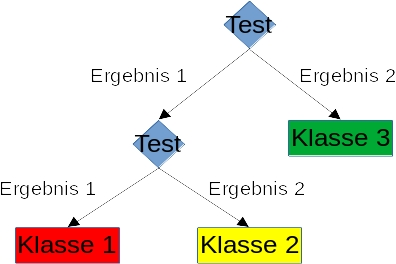
\includegraphics[width=0.5\linewidth]{images/entscheidungsbaum.jpg}
    \caption{Beispiel eines binären Entscheidungsbaums mit 3 möglichen Klassen, die klassifizierbar sind.}
    \label{fig:entscheidungsbaum}
\end{figure}
Der Entscheidungsbaum ist eine rekursive Datenstruktur um Entscheidungsregeln darzustellen. Jedem Blatt ist eine Klasse zugeordnet und allen anderen Knoten ist ein \textit{Test} zugeordnet. Der Test hat eine Reihe von sich
gegenseitig auschließenden Ergebnissen. Die Zuordnung einer Klasse zu einem Objekt wird durch das Traversieren dieses Baumes bestimmt bis ein Blatt erreicht wird \cite{quinlan1990decision}. Abbildung \ref{fig:entscheidungsbaum}
zeigt einen Entscheidungsbaum, wo jeder Test zwei mögliche Ergbnisse hat, i. e. einen binären Entscheidungsbaum. Möglich wäre aber auch das jeder Test eine arbiträre Anzahl an möglichen Ergebnissen hätte.

\subsection{Konstruktion}
\label{sec:construction}
Es gibt viele verschiedene Algorithmen um Entscheidungsbäume zu erzeugen: \texttt{ID3}, \texttt{C4.5}, \texttt{C5}, \texttt{CART}, \texttt{CHAID}, \texttt{QUEST},
\texttt{GUIDE}, \texttt{CRUISE} and \texttt{CTREE}. Am häufigsten wird ID3 (Iterative Dichotomizer 3), bzw. C4.5, welches eine Weiterentwicklung von ID3 ist, und CART (Classification and Regression Trees) verwendet \cite{scikit-learn, singh2014comparative}.
Diese Arbeit verwendet die Implementierung für Entscheidungsbaumklassifizierer von \textit{Scikit-Learn}, die eine optimierte Version von CART nutzt \cite{ScikitLearnCART}. Scikit-Learn ist ein Python-Modul, das eine
große Auswahl von Algorithmen zum maschinellen Lernen implementiert \cite{scikit-learn}.

\subsubsection{CART: Classification and Regression Trees}
Die Konstruktion eines optimalen binären Entscheidungsbaum ist NP-Komplett \cite{laurent1976constructing}. CART ist ein Greedy-Algorithmus, der lokal immer die beste Teilung wählt.
\begin{lstlisting}[label=lst:CARTtreeGrowing,caption={Skizze von vereinfachten Baumwachstumsalgorithmus \cite{steinbergCART}.}]
    Weise dem Wurzelknoten alle Trainingsdaten zu.
    Definiere den Wurzelknoten als Blatt.
    WHILE True:
        Neue_Teilungen = 0
        FOR jedes Blatt:
            IF die Größe der zugewiesenen Trainingsdaten zu klein ist oder alle Einträge der Trainingsdaten zur gleichen Klasse gehören:
                CONTINUE
            Finde das Attribut, das am besten den Knoten in zwei Kindesknoten unterteilt mit einer erlaubten Teilungsregel.
            Neue_Teilungen += 1
        IF Neue_Teilungen == 0:
            break
\end{lstlisting}
Listing \ref{lst:CARTtreeGrowing} skizziert wie CART initial einen maximal großen Baum generiert indem die Trainingsdaten solange geteilt werden bis keine weitere Teilung mehr möglich ist oder alle Einträge der gleichen
Klasse zugeordnet sind. Zuletzt beginnt der Reduzierungsprozess indem Teilbäume gelöscht werden, die die Klassifizierungsgenauigkeit nicht erhöhen oder der Zuwachs unter einem Nutzer definierten
Schwellenwert liegt \cite{steinbergCART}.
\section{Ensemble-Methoden}
Oftmals ist der Suchraum für das Problem zu groß, als das es möglich wäre in tolerabler Zeit die optimale Lösung zu finden \cite{laurent1976constructing}. Konstruktionsalgorithmen für Entscheidungsbäume arbeiten aus
diesem Grund auf Basis von Heuristiken um die lokal optimale Teilung zu bestimmen. Im Gegensatz zu diesen Algorithmen versuchen Ensemble-Methoden nicht die beste Lösung, sondern konstruieren eine Menge von Lösungen
unter denen anschließend gewählt wird, was die finale Lösung für ein Problem ist \cite{dietterich2002ensemble}.

\subsection{Voting}
\subsection{Bagging}
\begin{figure}
    \centering
    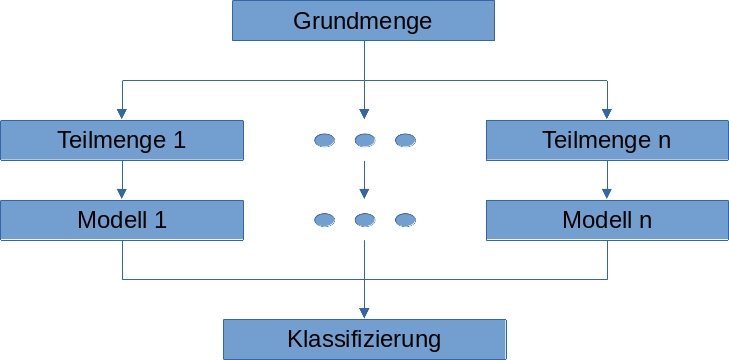
\includegraphics[width=0.6\linewidth]{images/bagging.jpg}
    \caption{Klassifizierungsprozess mit der Bagging-Methode.}
    \label{fig:bagging}
\end{figure}
Bagging ist ein Acronym für \glqq \textbf{B}ootstrap \textbf{agg}regat\textbf{ing}\grqq. Die Idee ist aus einer großen Menge von Trainingsdaten, eine Menge von Mengen von Trainingsdaten zu generieren, folgend mit jedem
dieser Mengen einen Klassifizierer zu trainieren und schließlich alle Klassifizierer, e.g. durch Wählen, zu aggregieren (siehe Abbildung \ref{fig:bagging}) \cite{breiman1996bagging}. Die Methode die dahinter steht nennt
sich \glqq Bootstrap sampling\grqq, welche einen Prozess beschreibt aus einer Grundmenge $m$ mal jeweils $n$ Einträge zu ziehen, die eine Teilmenge bilden \cite{efron1992bootstrap}. Der Name ist folglich aus der Methode
und dem Aggregierungsprozess abgleitet.
\subsection{Random Forest}
Random Forest ist eine Erweiterung der Bagging-Methode. Zusätzlich zu der zufällig ausgewählten Menge an Trainingsdaten wird auch zufällig eine Menge von Features ausgewählt. Auf dieser Basis wird ein Menge von
Entscheidungsbäumen generiert die anschließend aggregiert werden \cite{breiman2001random}.
\subsection{Boosting?}
\chapter{Stand der Forschung}
Dieses Kapitel verschafft einen Überblick über bisherige Arbeiten im Bereich der Gestenerkennung. Zuerst wird allgemein auf die Gestenerkennung mit Entscheidungsbäumen eingegangen. Anschließend wird der Ansatz
zur optischen Gestenerkennung vorgestellt, der im Institut für Telematik an der TUHH entwickelt wurde. Zuletzt wird auf die Ergebnisse von bisherigen Arbeiten mit künstlichen neuronalen Netzen mit diesem Ansatz eingegangen.

\section{Ähnliche Arbeiten}
Es gibt viele Ansätze, die sich mit der Gestenerkennung beschäftigen. Es wird unterschieden zwischen optischen und nicht-optischen Ansätzen. Der optische Ansatz nutzt einen
oder mehrere Kameras um eine Folge von Bildern aufzunehmen. Dieser Ansatz ist allerdings empfindlich gegenüber Lichtverhältnisse und der Distanz die der
Nutzer zu den Kameras hat \cite{song2019design}. Nicht-optische Ansätze bedienen sich anderen Sensoren, z. B. Infrarot Abstandssensoren \cite{cheng2011contactless},
oder nutzen technische Hilfsmittel um zusätzliche Daten zu erfassen.
\newline
\newline
Song et al. \cite{song2019design} haben die Handgestenerkennung mit Gradient Boosting Entscheidungsbäumen untersucht. Sie wählten einen nicht-optischen Ansatz, der aus einen tragbaren sEMG Recorder
der die elektrischen Signale der Muskelaktivitäten erfasst. Als Eingabe für den Entscheidungsbaum wählten sie neun Features die in die Kategorie von zeitabhängigen Features einzuordnen sind
(siehe Tabelle \ref{tab:songFeatures}). Damit erzielten sie eine Erkennungsgenauigkeit von 91\% unter 12 verschiedenen Handgesten.
\begin{table}[h!]
    \centering
    \begin{tabular}{ c | c | c }
        \hline
        \hline
        1 & Mean absolute value & $\frac{1}{N}\sum^N_{t=1} |x_t|$ \\\hline
        2 & Simple square integral & $\sum^N_{t=1} |x_t|^2$ \\\hline
        3 & Minimum value & $\min x_t$ \\\hline
        4 & Maximum value & $\max x_t$ \\\hline
        5 & Standard deviation & $\sqrt{\frac{1}{N}\sum^N_{t=1}(x_t - \tilde{x})^2}$ \\\hline
        6 & Average amplitude change & $\frac{1}{N-1}\sum^{N-1}_{t=1} |x_{t + 1} - x_t|$ \\\hline
        7 & Zero crossing & $\sum^{N-1}_{t=1}diff(sgn(x_{t+1}),sgn(x_t))$ \\\hline
        8 & Slope sign change & $\sum^{N-2}_{t=1}diff(sgn(x_{t+1} - x_t),sgn(x_t - x_{t - 1}))$ \\\hline
        9 & Willison amplitude & $\sum^{N-1}_{t=1}u(|x_{t+1} - x_t| - threshold)$ \\
        \hline
        \hline
    \end{tabular}
    \caption{Die von Song et al. genutzten Features \cite{song2019design}.}
    \label{tab:songFeatures}
\end{table}
\newline
\newline
Ahad et al. \cite{ahad2012motion} diskutieren den Motion History Image (MHI) Ansatz. MHI ist ein optischer Ansatz, der eine Sequenz von Bildern in ein einziges komprimiert. Dabei werden dominate Bewegungen die
kürzlich verarbeitet wurden heller angezeigt als nicht dominate Bewegungen oder Bewegungen die schon länger zurück liegen.
\begin{align}
    H_{\tau}(x,y,t) = \begin{cases}
                          \tau & if \psi(x,y,t) = 1 \\
                          \max(0, H_{\tau}(x,y,t-1) - \delta) & otherwise
    \end{cases}
    \label{formular:mhi}
\end{align}
Das MHI kann sequentiell berechnet werden. Initial sind alle Werte 0. Wenn $\psi(x,y,t)$ eine dominate Bewegung in einem Pixel $(x,y)$ zu einem Zeitpunkt $t$ signalisiert, dann wird der Pixel zum Maximalwert $\tau$
gesetzt. Mit jedem Bild in denen keine dominate Bewegung im Pixel $(x,y)$ stattgefunden hat, wird der Wert um den Zerfallswert $\delta$ dekrementiert bis zu einem Minimum von 0 (siehe Formel \ref{formular:mhi}).
\newline
\newline
MHI ist leicht zu berechnen und Invariant zu Lichtverhältnissen. Allerdings ist die Leistung stark abhängig von $\psi$, $\tau$ und $\delta$. MHI ist besonders anfällig für Bildfolgen mit verschiedener Länge.
Jenachdem wie $\tau$ und $\delta$ gewählt sind, ist die Bewegungshistorie nicht sichtbar oder verloren gegangen.
\section{Optische Handgestenerkennung}
\label{sec:fallstudie}
\begin{figure}
    \centering
    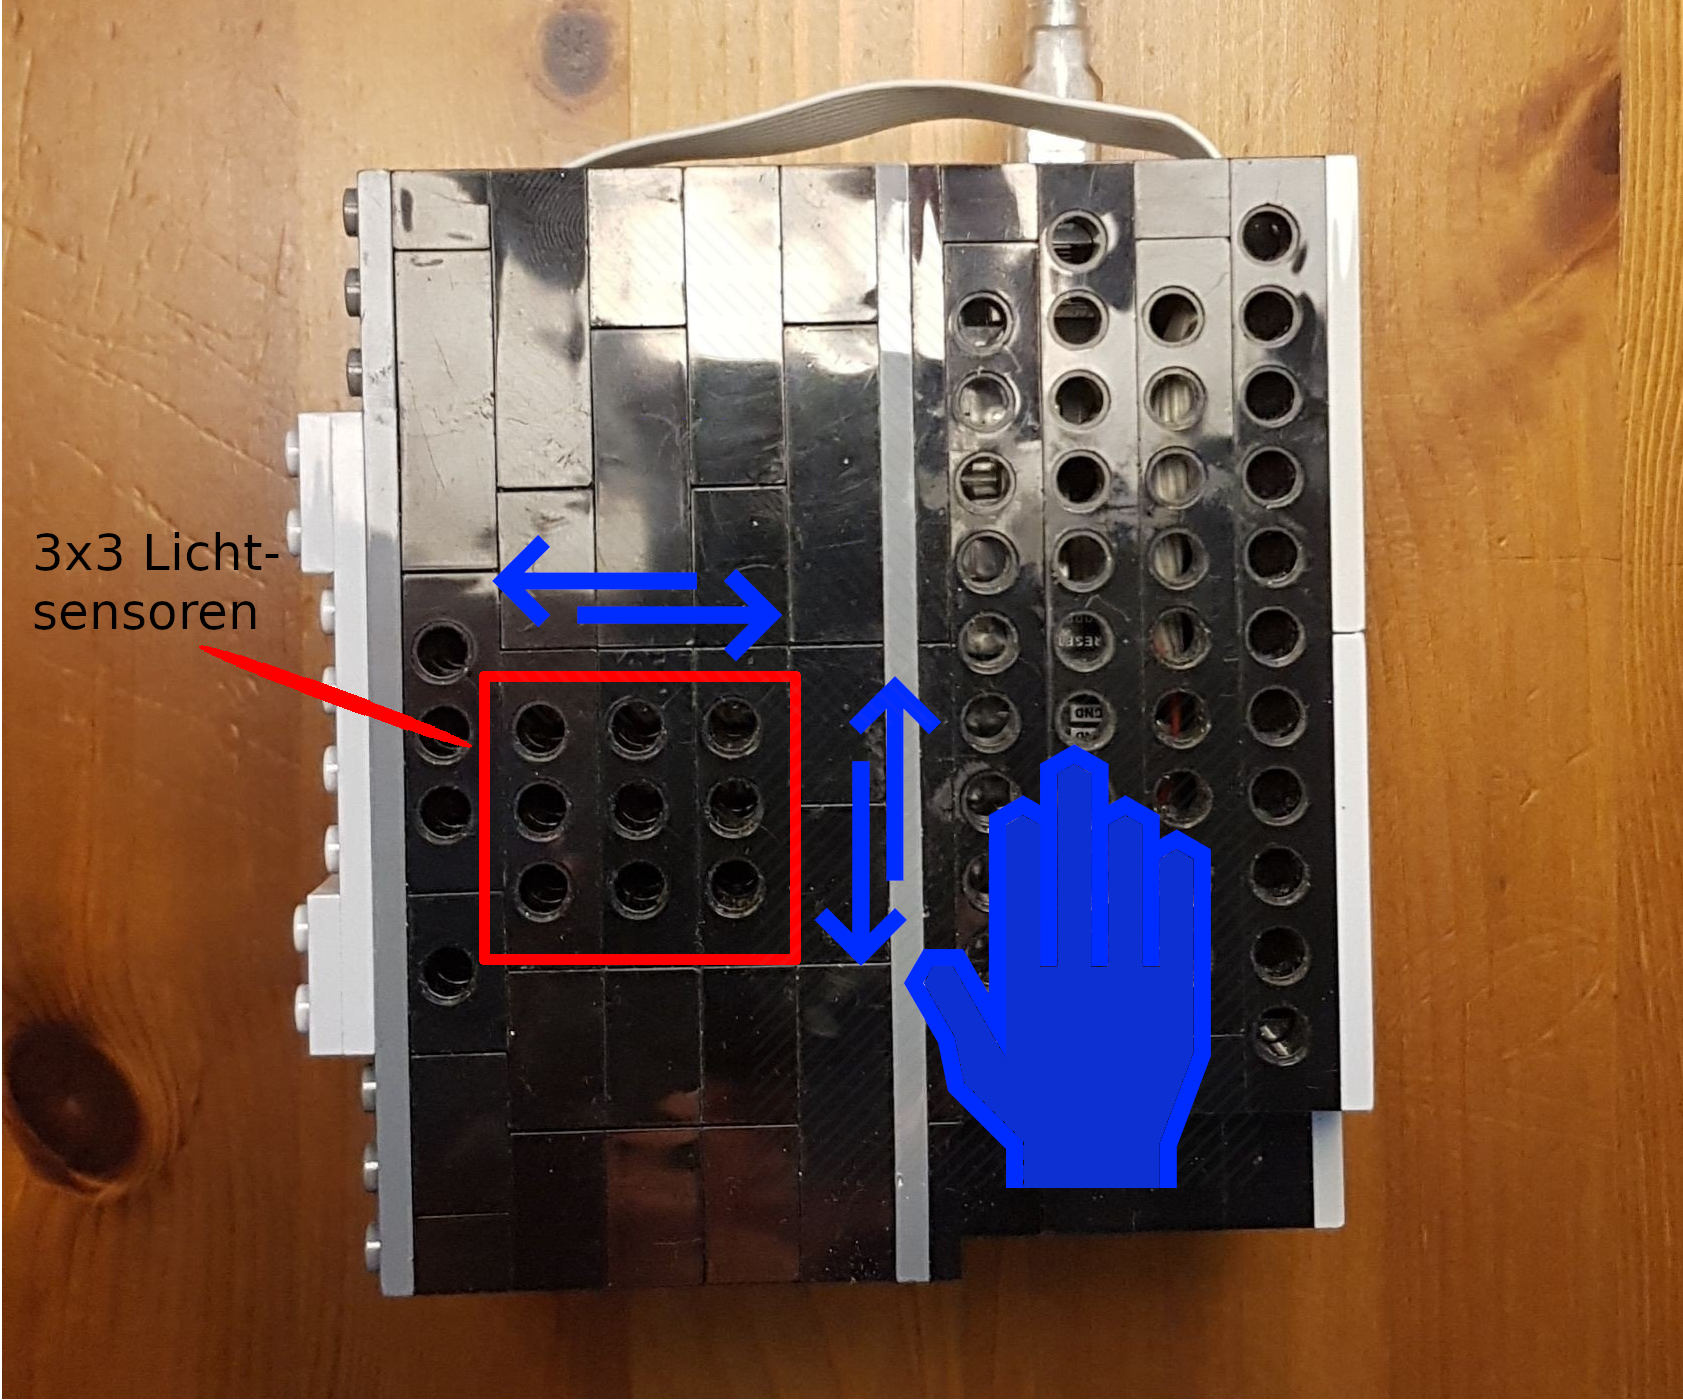
\includegraphics[width=0.6\linewidth]{images/arduino_ex.png}
    \caption{Das Arduino-Board ATmega328P mit 3x3 Matrix von Lichtsensoren in Lego-Verpackung. Illustriert werden die möglichen Handgestentypen mit Ausnahme der Nullgeste.}
    \label{fig:arduino_ex}
\end{figure}
Diese Arbeit ist Teil einer Fallstudie zur Handgestenerkennung auf Low-End Mikrocontrollern von dem Institut für Telematik an der TUHH \cite{venzkeArticle}. Das Ziel ist die Handgestenerkennung in Echtzeit mit so wenig
Ressourcen wie möglich, damit die Produktion der einzelnen Module so kostengünstig wie möglich ist. Als Eingabe dient, je nach Modul, eine 3x3, bzw. 4x4, Matrix von Lichtsensoren. Abbildung \ref{fig:arduino_ex}
illustriert 4 Typen von Handgesten, die über den Mikrocontroller ausgeführt werden: Links nach Rechts, Rechts nach Links, Oben nach Unten, Unten nach Oben. Zudem wird zwischen Handgesten und Nullgesten, d. h.
invalide Handgesten, unterschieden. In den bisherigen Arbeiten wurden ML Modelle mit künstlichen neuronalen Netzwerken erstellt. Dessen Prozessablauf zur Handgestenerkennung lässt sich auf 3
Schritte zusammenfassen.
\begin{enumerate}
    \item Extrahiere einen Gestenkandidaten.
    \item Vorverarbeite den Gestenkandidaten.
    \item Wende das Modell auf den vorverarbeiteten Gestenkandidaten an.
\end{enumerate}

\subsection{Exrahierung von Gestenkandidaten}
Die Lichtsensorenmatrix liefert einen kontinuierlichen Strom an Bildern. Dabei limitiert die Verarbeitungszeit eines Bildes die Anzahl an Bilder pro Sekunde. Als Gestenkandidat wird eine Folge von Bildern definiert, die
ein Ereignis einschließt. In diesem Fall wird das Ereignis durch die Veränderung im gleitenden Mittelwert der Lichtverhältnisse definiert, i. e. sobald der gleitende Mittelwert unterschritten wird ein Gestenkandidat
angefangen aufgenommen zu werden und sobald die Lichtverhältnisse zu dem Wert zurückkehren wird die Aufnahme beendet. Der gleitende Mittelwert wird dabei immer angepasst, wenn kein Gestenkandidat aufgenommen wird, um
sich den veränderden Lichtverhältnissen anzupassen. Da leichte Veränderungen natürlich sind, muss eine Toleranzgrenze von 10\% unterschritten werden, damit die Aufnahme gestartet wird. Dies hat als Folge, dass der Anfang
und das Ende nicht vollständig ist. Aus diesem Grund schlug Kubik zusätzlich vor am Anfang und Ende weitere Bilder anzufügen \cite{kubikThesis}.
\newline
\newline
\begin{figure}
    \usetikzlibrary{arrows,automata,positioning}
    \centering
    \begin{tikzpicture}[
        block/.style={
        draw,
        fill=white,
        text width=0.14*\columnwidth,
        anchor=west,
        minimum height=1cm,
        rounded corners
        },
        font=\small,
        on grid, auto,
        node distance=5cm
    ]
        \node [block,align=center,initial] (s0) {READ-INITIAL-FRAMES};
        \node [block,align=center] (s1) [right of=s0] {SEARCH-DARKER-FRAMES};
        \node [block,align=center] (s2) [right of=s1] {RECORD-CANDIDATE-FRAMES};
        \node [block,align=center] (s3) [below of=s2] {RECORD-ENDING-FRAMES};
        \node [block,align=center, node distance=6cm] (s4) [left of=s3] {GESTURE-CANDIDATE-CLASSIFIED};
        \path [->, text width=2cm, align=center] (s0) edge [loop below] node {\#Bilder<3: BGMH} (s0);
        \path [->, text width=2cm, align=center] (s0) edge node {\#Bilder=3: BGMH} (s1);
        \path [->, text width=4cm, align=center] (s1) edge [loop below] node {ØHelligkeit$\geq$GMH$\cdot 0.9$: BGMH, pop\_first(Bilder)} (s1);
        \path [->, text width=3cm, align=center] (s1) edge node {ØHelligkeit < GMH$\cdot 0.9$} (s2);
        \path [->, text width=2cm, align=center] (s2) edge node {ØHelligkeit $\geq$ GMH$\cdot 0.9$: AnzahlEndBilder:=3} (s3);
        \path [->, text width=3cm, align=center] (s3) edge [loop below] node {AnzahlEndBilder>0: AnzahlEndBilder-=1} (s3);
        \path [->, text width=3cm, align=center] (s3) edge node {AnzahlEndBilder=0} (s4);
        \path [->] (s4) edge node {Variablen zurücksetzen} (s0);
    \end{tikzpicture}
    \caption{Implementierung von Kubik's Algorithmus um Gestenkandidaten zu erkennen von Dr. Marcus Venzke. BGMH steht für die Aktion \glqq \textbf{B}erechnung \textbf{G}leitender \textbf{M}ittelwert der \textbf{H}elligkeit\grqq und GMH steht für die Variable \glqq \textbf{G}leitender \textbf{M}ittelwert der \textbf{H}elligkeit\grqq.}
    \label{fig:venzkeAlgoImpl}
\end{figure}
Abbildung \ref{fig:venzkeAlgoImpl} zeigt die konkrete Implementierung dieses Algorithmus mit einem Zustandsautomaten von Dr. Marcus Venzke. In jedem Zustand wird das aktuelle Bild dem Puffer angefügt. Der Automat
verbleibt im Zustand \texttt{READ-INITIAL-FRAMES} bis der Puffer 3 Bilder enthält und passt stets den gleitenden Mittelwert der Helligkeit an. Anschließend geht der Automat in den Zustand
\texttt{SEARCH-DARKER-FRAMES} über, indem er weiterhin den gleitenden Mittelwert anpasst und immer das erste Bild aus dem Puffer entfernt, da lediglich 3 Bilder jeweils vorm Aufnehmen und nach dem Aufnehmen des
Gestenkandidates angefügt werden sollen. Sobald die Durchschnittshelligkeit den 90\% des gleitenden Mittelwerts unterschreitet wird die Aufnahme begonnen. Der Automat geht in den Zustand \texttt{RECORD-CANDIDATE-FRAMES}
über. Dort verbleibt der Automat solange bis die Durchschnittshelligkeit 90\% des gleitenden Mittelwerts überschreitet, woraufhin der Automat in den Zustand \texttt{RECORD-ENDING-FRAMES} über geht, indem die letzten 3
Bilder an den Puffer angehängt werden. Der Zustand des Puffers im Zustand \texttt{GESTURE-CANDIDATE-CLASSIFIED} repräsentiert den Gestenkandidaten. Zuletzt werden alle nötigen Variablen zurückgesetzt und der
Automat geht in den initialen Zustand wieder über.
\section{Skalieren des Gestenkandidaten}
\label{sec:scaling}
Ein Gestenkandidat besteht aus einer variablen Anzahl von Bildern. Durch die künstlich angefügten Bilder am Anfang und Ende sind es mindestens acht Bilder. Kubik erkannte, dass ein neuronales Netz eine feste Anzahl an
Eingaben benötigt und diskutierte verschiedene Ansätze, um mit einer variablen Länge des Input umzugehen. Er verwarf die Idee den Puffer mit irrelevanten Bildern oder Nullen auszufüllen, Bilder zu duplizieren
oder Teile des Gestenkandidaten zu verwerfen. Er befürchtete, dass dadurch nicht die vollständige Handgeste auf die Eingangs-Ebene des neuronalen Netzes (NN) abgebildet werden würde, oder dass die Handgeste
womöglich verzerrt wäre \cite{kubikThesis}.
\newline
\newline
Kubik schlug vor, dass lineare Interpolation angewendet werden soll. Dabei werden die vorhandenen Bilder uniform auf 20 Pseudoindexe verteilt, sodass das erste und letzte Bild auch
jeweils den ersten und letzten Pseudoindex einnimmt. Die übrigen Indize sind gleich verteilt. Aus diesem Grund ergeben sie nicht immer natürliche Zahlen. In diesem Fall wird das Bild durch Interpolation des
vorherigen Bildes und des nächsten Bildes erzeugt. Dieser Ansatz wurde auch von Giese aufgegriffen, der sich in diesem Zusammenhang
ebenfalls mit künstlichen neuronalen Netzen beschäftigt hatte \cite{gieseThesis}.
\subsection{Trainingsdaten}
\subsection{Gestenerkennung mit künstliche neuronalen Netzen}
Insgesamt gingen dieser Arbeit 4 Arbeiten voraus, die sich mit künstlichen neuronalen Netzen im Zusammenhang dieser Fallstudie beschäftigt hatten.

\subsubsection{Engelhardt}
Engelhardt führte die in \ref{sec:fallstudie} definierten Handgesten mit der Hand, einem Finger und 2 Finger unter verschiedenen Helligkeiten aus, auf Basis dessen seine Modelle trainiert und validiert wurden. Er
argumentiert, dass rekurrente neuronale Netze (RNN), Feedforward neuronale Netze (FFNN) und Long-Short-Term Memory neuronale Netze (LSTMNN) am besten geeignet für temporale Probleme seien. Convolutional neuronale
Netze (CNN) verwarf Engelhardt aufgrund der geringen Auflösung der Gesten und da die Faltung extrem Rechenaufwendig sei. Desweiteren verwarf er LSTMNN, da diese zu viel Rechenleistung und Speicherplatz
benötigen. Als Eingabewerte zu seinen RNNs und FFNNs diente eine Sequenz von 20 Bilder die zu 180 Werten konkatiniert wurden und auf Werte zwischen 0 und 1 normalisiert wurden. Als bestes Model stellte sich eines
seiner FFNNs heraus, das auf seinen Testdaten bis zu 99\% Erkennungsgenauigkeit erzielte. Außerdem erwies es sich als robust gegenüber Rauschen und Helligkeitsveränderungen im Vergleich zum RNN. Die Ausführungszeit
des FFNN belief sich auf 11,54 ms mit einem Verbrauch von 11 kB Flash-Speicher und 573 bytes RAM \cite{engelhardtThesis}.

\subsubsection{Kubik}

\subsubsection{Klisch}

\subsubsection{Giese}

\chapter{Achievements}
TODO Also talk somwhere about the training sets
\section{Erstellte Werkzeuge und Bibliotheken}
\label{sec:recorder}
\begin{figure}
    \centering
    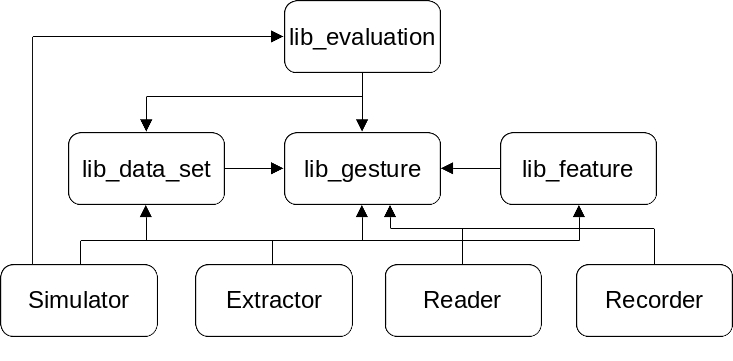
\includegraphics[width=0.75\linewidth]{images/architecture_overview.jpg}
    \caption{Abhängigkeitein der einzelnen Module.}
    \label{fig:architecture_overview}
\end{figure}
In dieser Arbeit mussten viele Features und Konfigurationen der Entscheidungsbäume untersucht und zu getestet werden. Aus diesem Grund wurde eine umfangreiche Infrastruktur geschaffen, die die
Auswertung von ML Modellen mit den Handgestendaten vereinfacht. Die Infrastruktur umfasst ein Datenmodel für Handgesten und kann die Datenmengen mit verschiedenen Parsingmethoden einlesen.
\newline
\newline
Außerdem können synthetischen Daten auf verschiedene Arten generiert werden. Die Architektur der Infrakstruktur erlaubt es weitere Features hinzuzufügen, ohne Kompatibilitätsprobleme zu verursachen.
Alle Funktionalitäten sind in Code-Bibliotheken isoliert, um die Integration in Hilfprogramme zu vereinfachen (siehe Abbildung \ref{fig:architecture_overview}).
\newline
\newline
Im folgenden wird die Funktionalität der einzelnen Module vorgestellt und die daraus erstellten Hilfsprogramme.
\newline
\newline
\texttt{lib\_gesture} definiert die Handgeste und die vorhandenen Gestentypen. Außerdem implementiert sie zwei Parsing-Methoden. Die erste Methode parsed Handgesten nach Annotation und die
zweite nach Kubiks Algorithmus (siehe Sektion \ref{sec:gesture_extraction}). Die Handgeste selber implementiert Methoden um synthetische Daten zu generieren.
\begin{itemize}
    \item Rotation um 90°, 180° und 270°.
    \item Nullgesten durch das Kombinieren der ersten Hälfte der Ausgangsgeste und der zweiten Hälfte von dessen Rotationen.
    \item Verschiebung der Pixel nach Oben und Unten für eine Links nach Rechts bzw. Rechts nach Links Geste und analog dazu eine Verschiebung nach Links und Rechts für die restlichen Handgesten.
    \item Rotation der äußeren Pixel um Diagonale Handgesten zu generieren.
\end{itemize}
\begin{lstlisting}[label=lst:FeatureInterface,caption={Interface, um ein Feature zu implementieren.}]
pub trait Feature {
    fn calculate(gesture: &Gesture) -> Self where Self: Sized;
    fn marshal(&self) -> String;
}
\end{lstlisting}
\texttt{lib\_feature} bietet ein einfaches Interface an um Feature mit einer Handgeste (siehe Listing \ref{lst:FeatureInterface}) zu implementieren. Zurzeit sind 28 verschiedene Feature implementiert.
\newline
\newline
\texttt{lib\_data\_set} stellt alle verfügbaren Datenmengen als statische Importe bereit. Einträge sind bereits nach Distanz zur Kamera, Helligkeit, Verdeckungsobjekt und Ausführungsgeschwindigkeit klassifiziert. Ein
Eintrag kann in der Helligkeit verändert werden entweder durch einen Offset oder indem er skaliert wird.
\newline
\newline
\texttt{lib\_evaluation} bietet ein Hilfsobjekt an, dass Datenmengen nach Erkennungsgenauigkeit auswertet und Berichte daraus generiert.
\newline
\newline
Der \texttt{Simulator} ist zweigeteilt. Der aktive Teil nutzt die die Gestenkandidatenerkennungsmethode nach Kubik, die in \texttt{lib\_gesture} implementiert ist, um den seriellen Datenstrom des Arduino zu parsen. Der
Gestenkandidat wird anschließend durch das hinterlegte Model klassifiziert und das Ergebnis ausgegeben. Der passive Teil evaluiert die Erkennungsgenauigkeit aller definierten Datenmengen.
\newline
\newline
Der \texttt{Extractor} extrahiert aus spezifizierten Datenmengen die definierten Features und exportiert diese in Dateien, sodass sie von dem Model zum Trainieren genutzt werden können. Optional kann die Datenmenge durch
sythetische Daten erweitert werden.
\newline
\newline
Der \texttt{Reader} gibt den seriellen Datenstrom des Arduino aus.
\newline
\newline
Der \texttt{Recorder} nutzt ähnlich wie der \texttt{Simulator} den seriellen Datenstrom des Arduino und die Parsingmethode von Kubik um Gestenkandidaten zu erkennen.
Diese Information wird genutzt, um in eine vordefinierte Datei die Handgesten reinzuschreiben. Um effizient Gesten aufzunehmen wurde der Ansatz von Kubik aufgegriffen mit
einem Gestentyp zu starten und folgend immer zwischen dem Inverstyp hin und her zu wechseln \cite{venzkeArticle}.
\newline
\newline
Das Programm wurde um zwei weitere Optionen erweitert. Mit der ersten Option wird immer nur eine bestimmte Handgeste hintereinander aufgenommen. Mit der zweiten Option wird jedes mal wenn eine Handgeste erkannt wurde,
der Gestentyp zur manuellen Eingabe erfragt. Mit disem Programm wurde die Datenmenge \texttt{DymelData} in wenigen Stunden erstellt (siehe Sektion \ref{sec:DymelData}).
\section{Aufgenommene Datenmenge}
\label{sec:DymelData}
\texttt{DymelData} ist eine Datenmenge, die mit dem \texttt{Recorder} (siehe Sektion \ref{sec:recorder}) erstellt wurde. Sie umfasst insgesamt 14410 Gesten in unterschiedlichen Konfigurationen. Sie wurde
einerseits aufgenommen, um unter den vorort bestehenden Lichtverhältnissen die Modelle miteinander vergleichen zu können und andererseits, um Test- und Trainingsdaten für Nullgesten bereitzustellen. In den
bisherigen Datenmengen enthält nur ein geringer Anteil Nullgesten.
\newline
\newline
\subfigbox{
\subfigure[Geringe Helligkeit]{\label{subfig:light_low}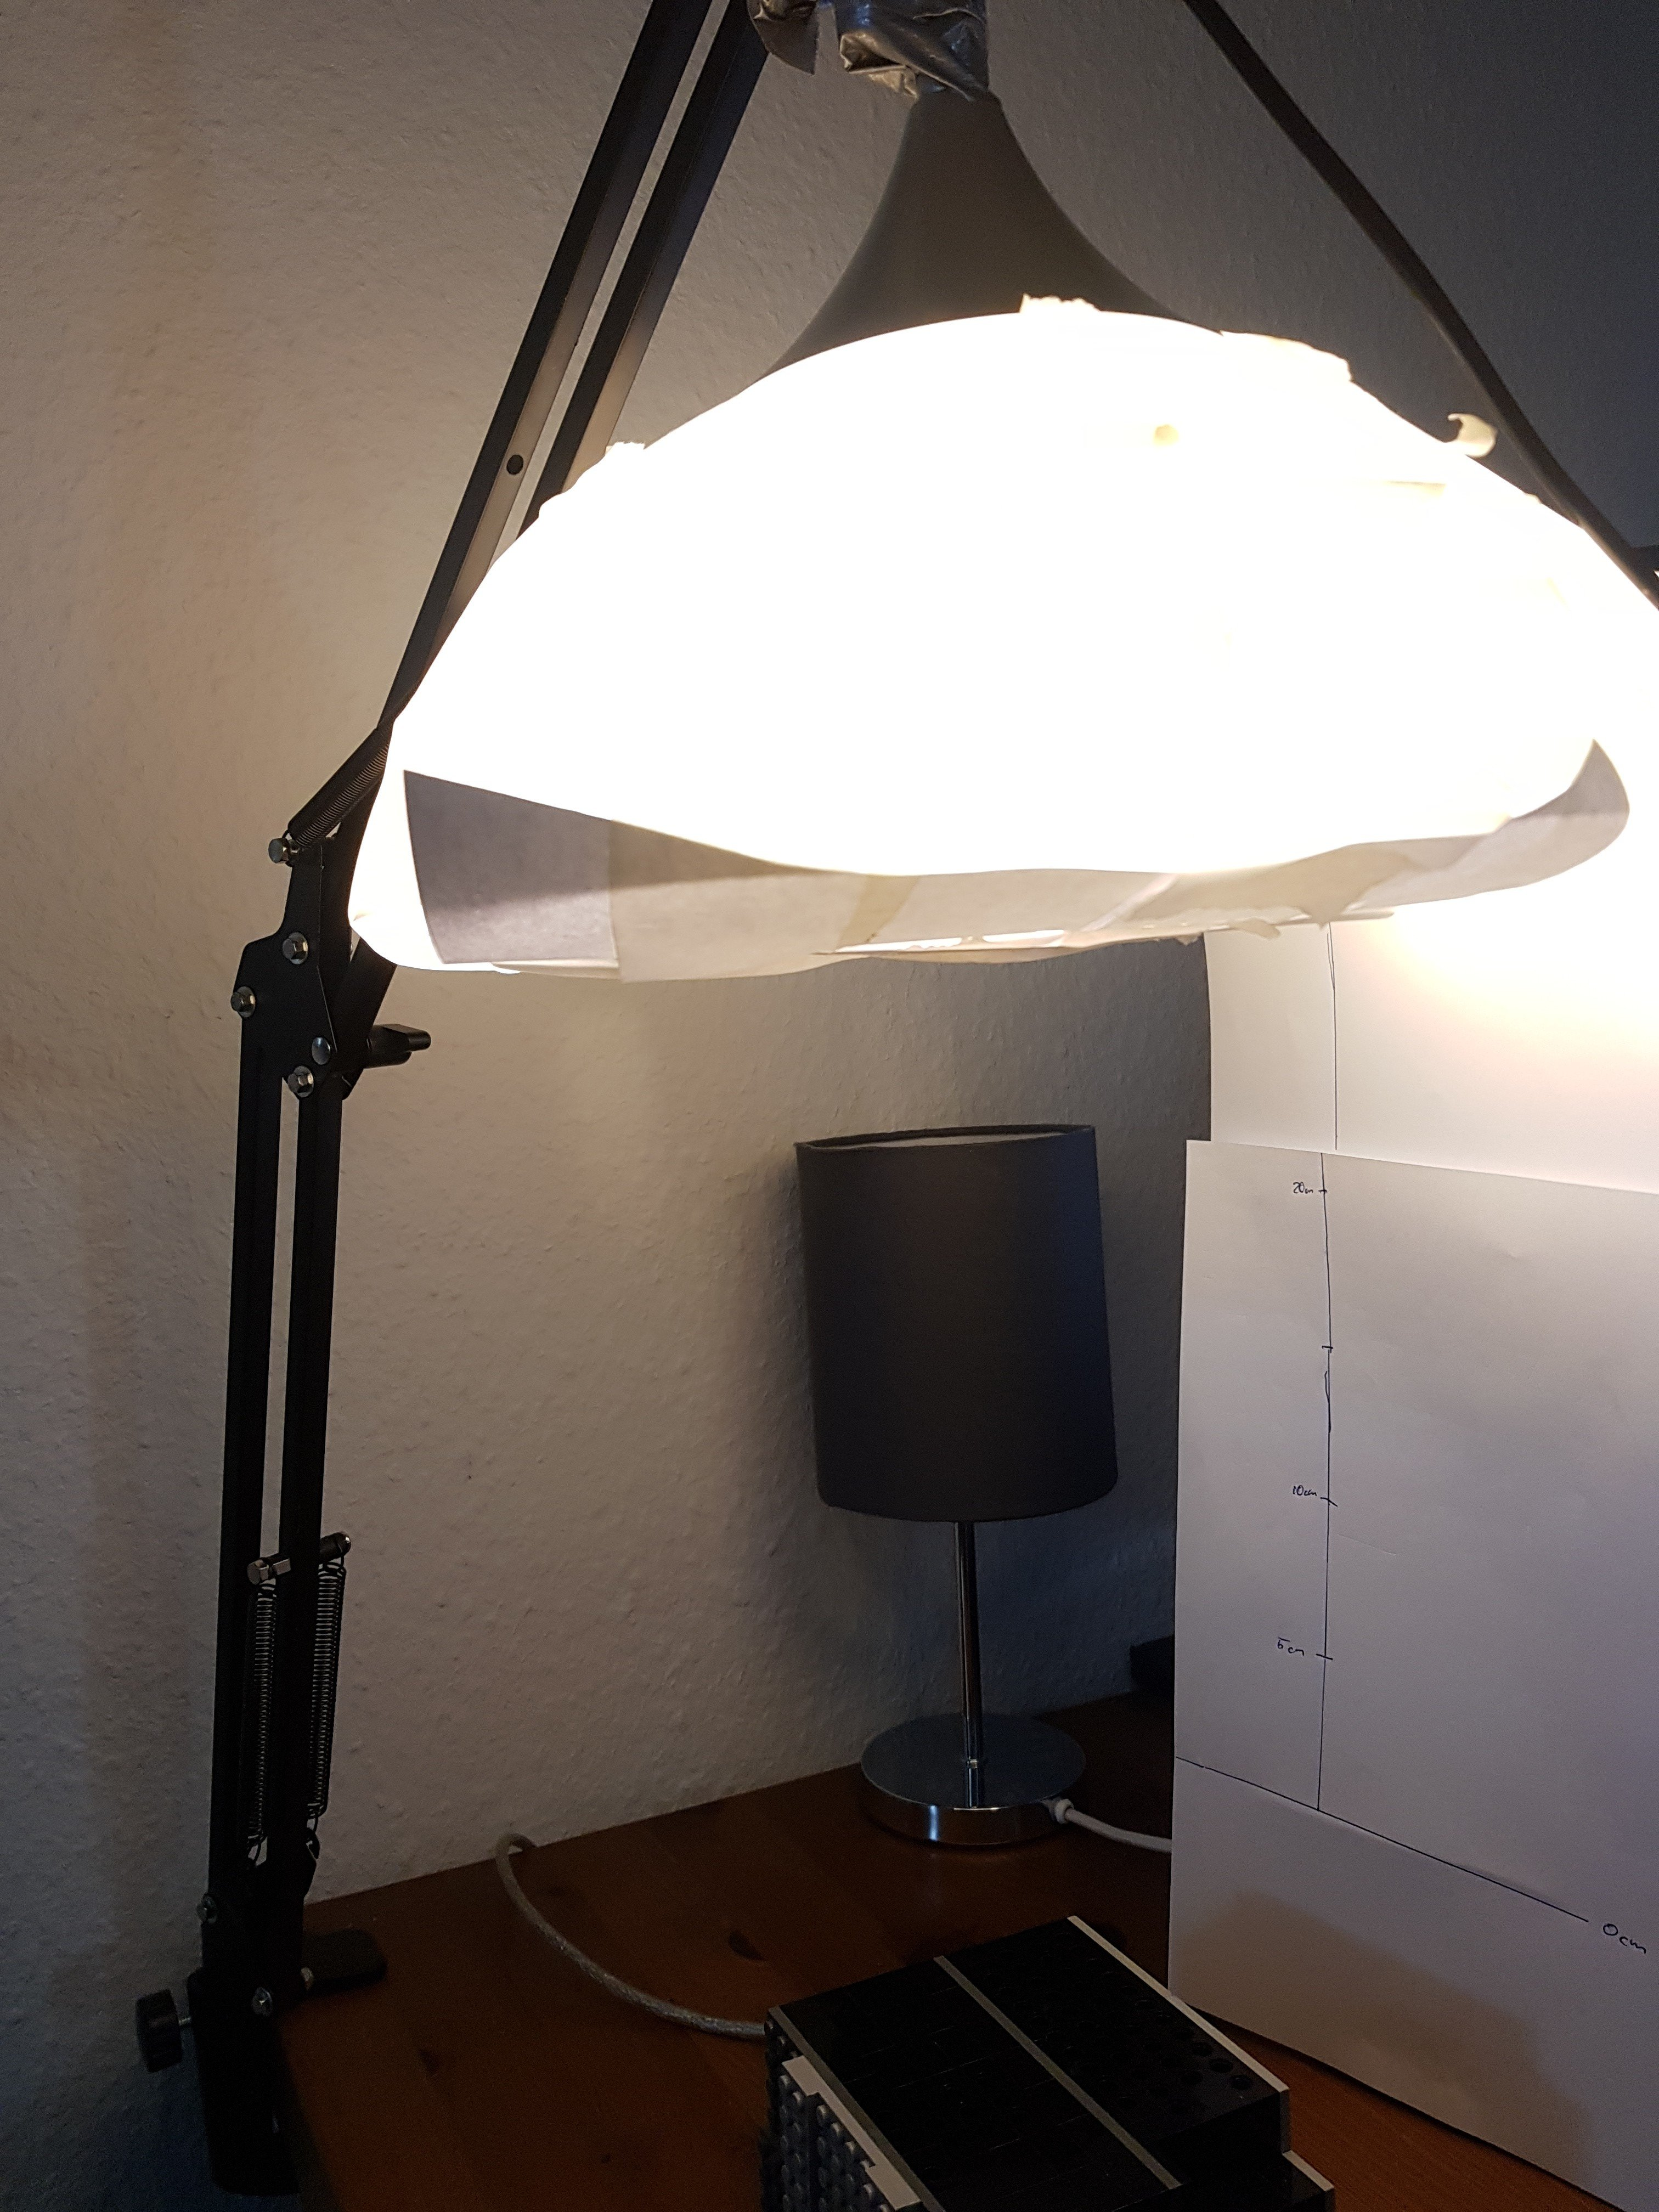
\includegraphics[width=0.33\linewidth]{images/light_low.jpeg}}\hfill%
\subfigure[Halbe Helligkeit]{\label{subfig:light_medium}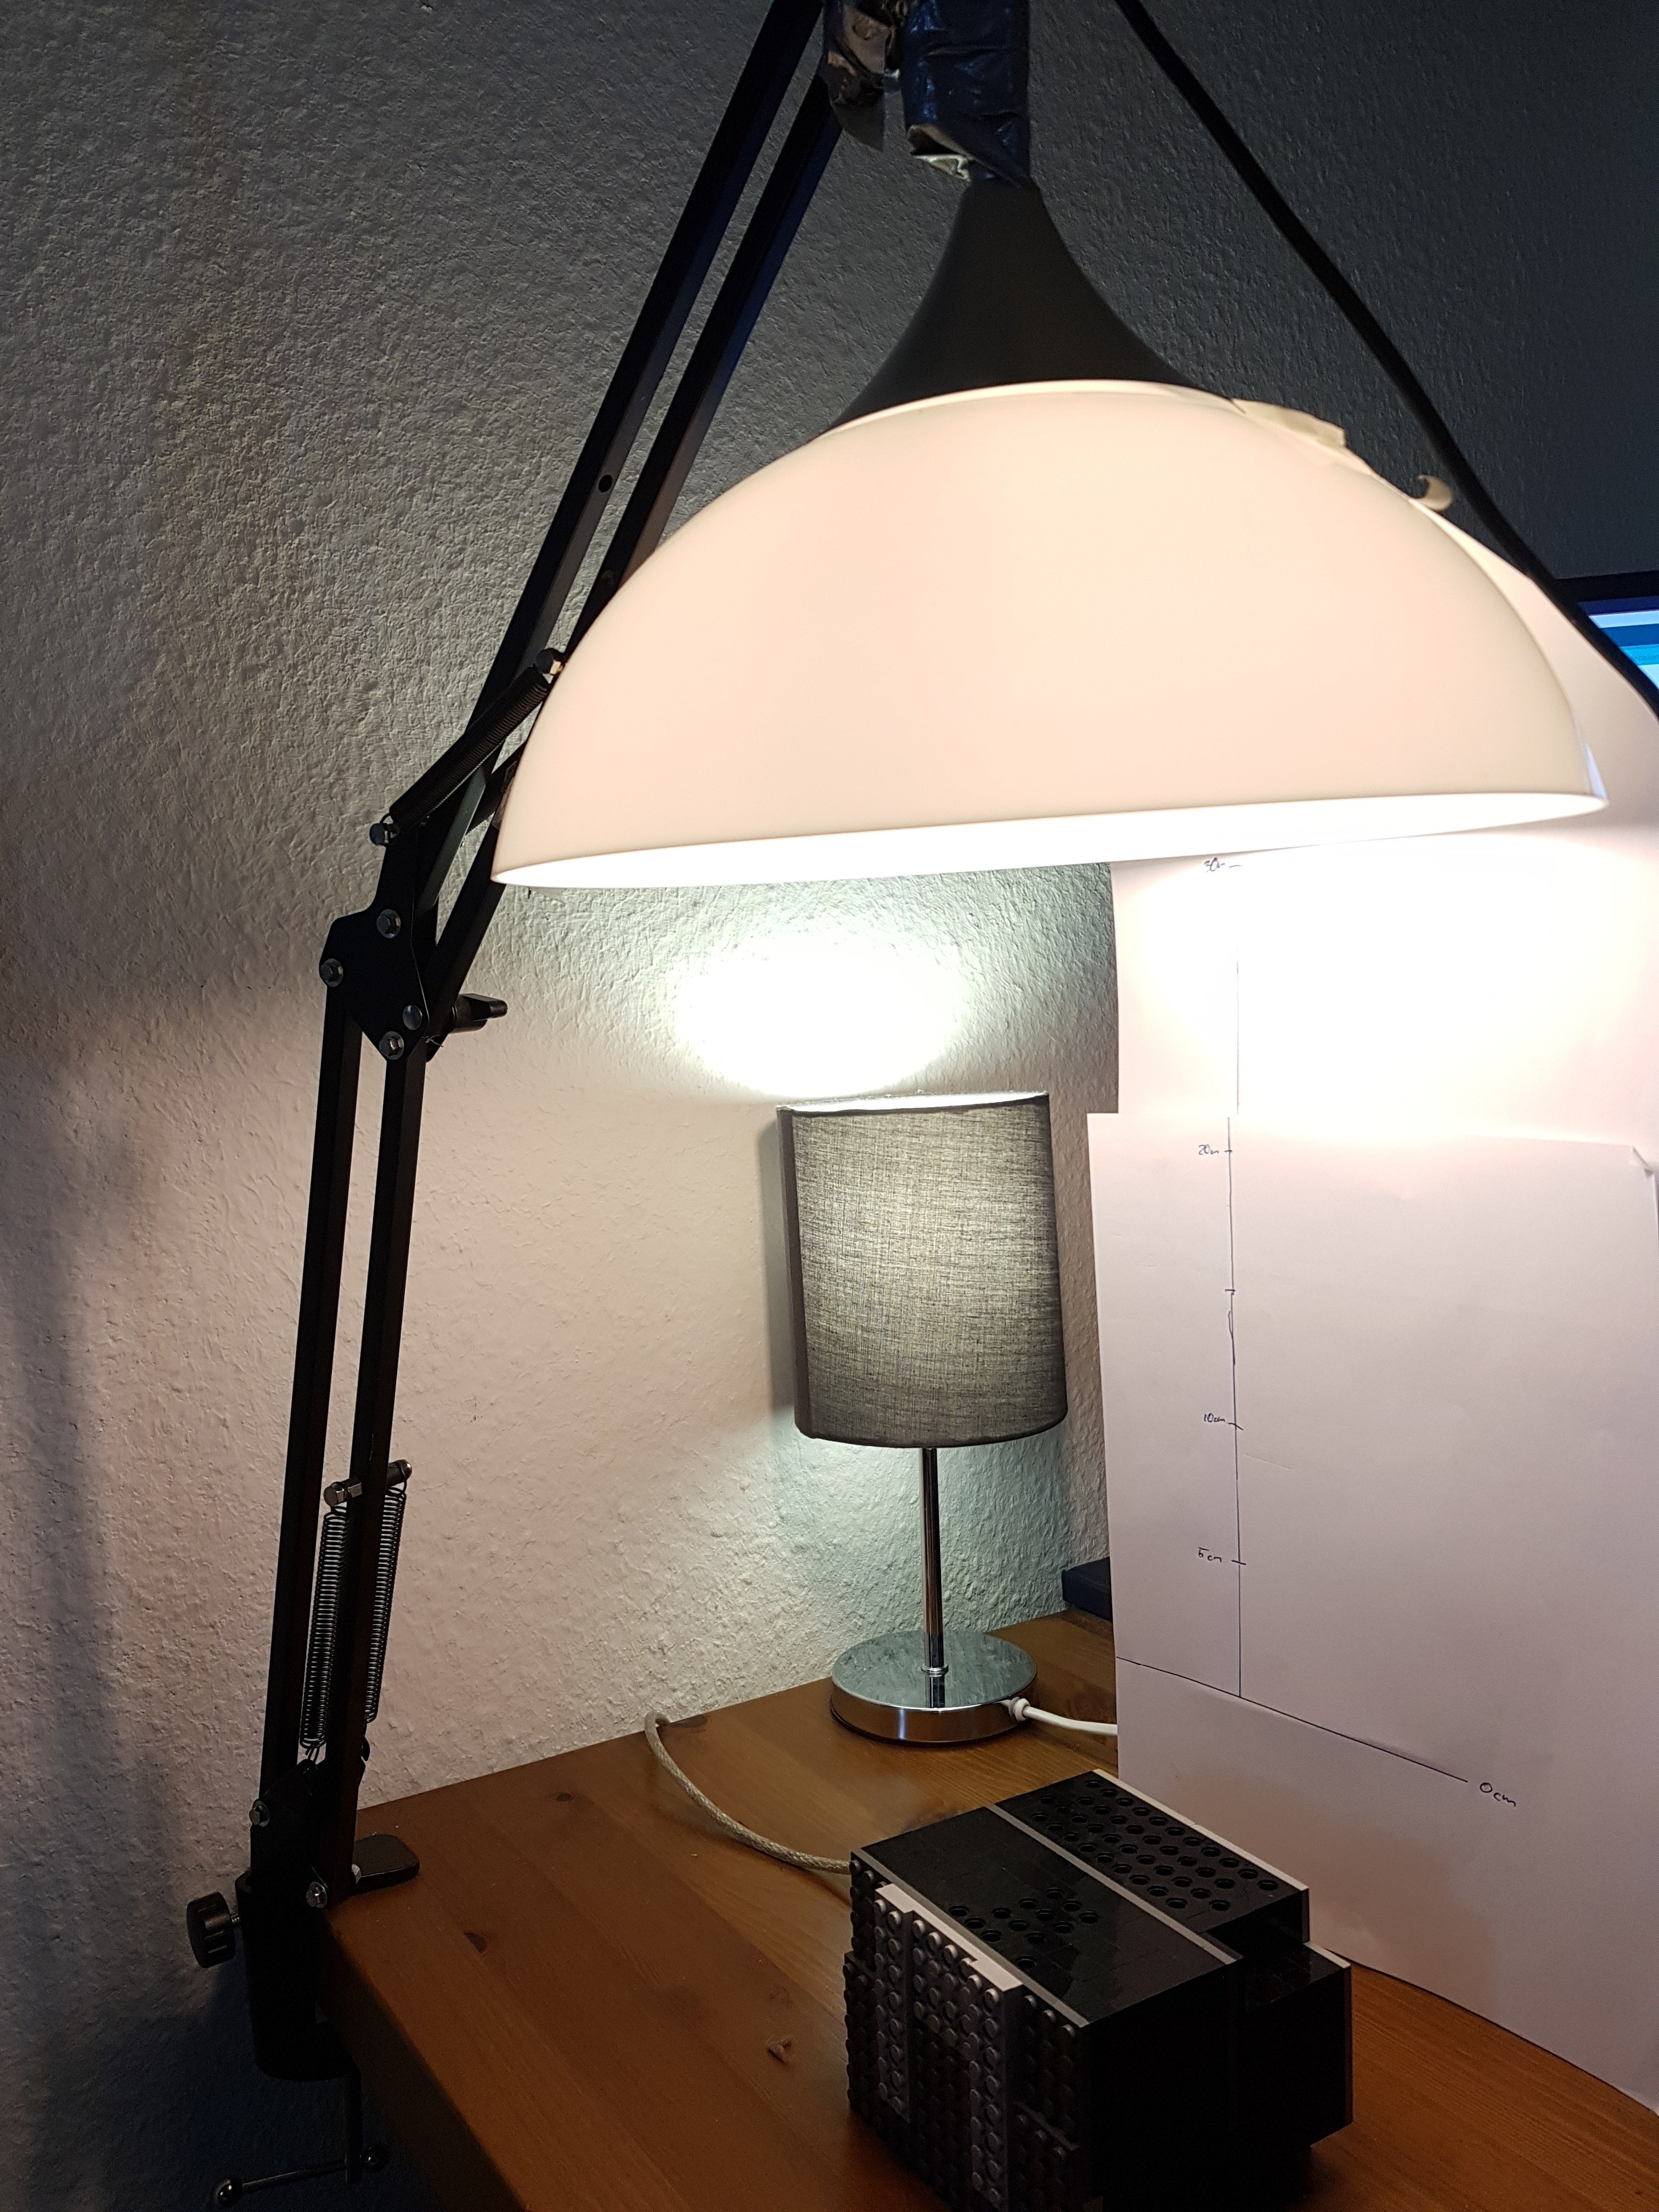
\includegraphics[width=0.33\linewidth]{images/light_medium.jpeg}}\hfill%
\subfigure[Hohe Helligkeit]{\label{subfig:light_high}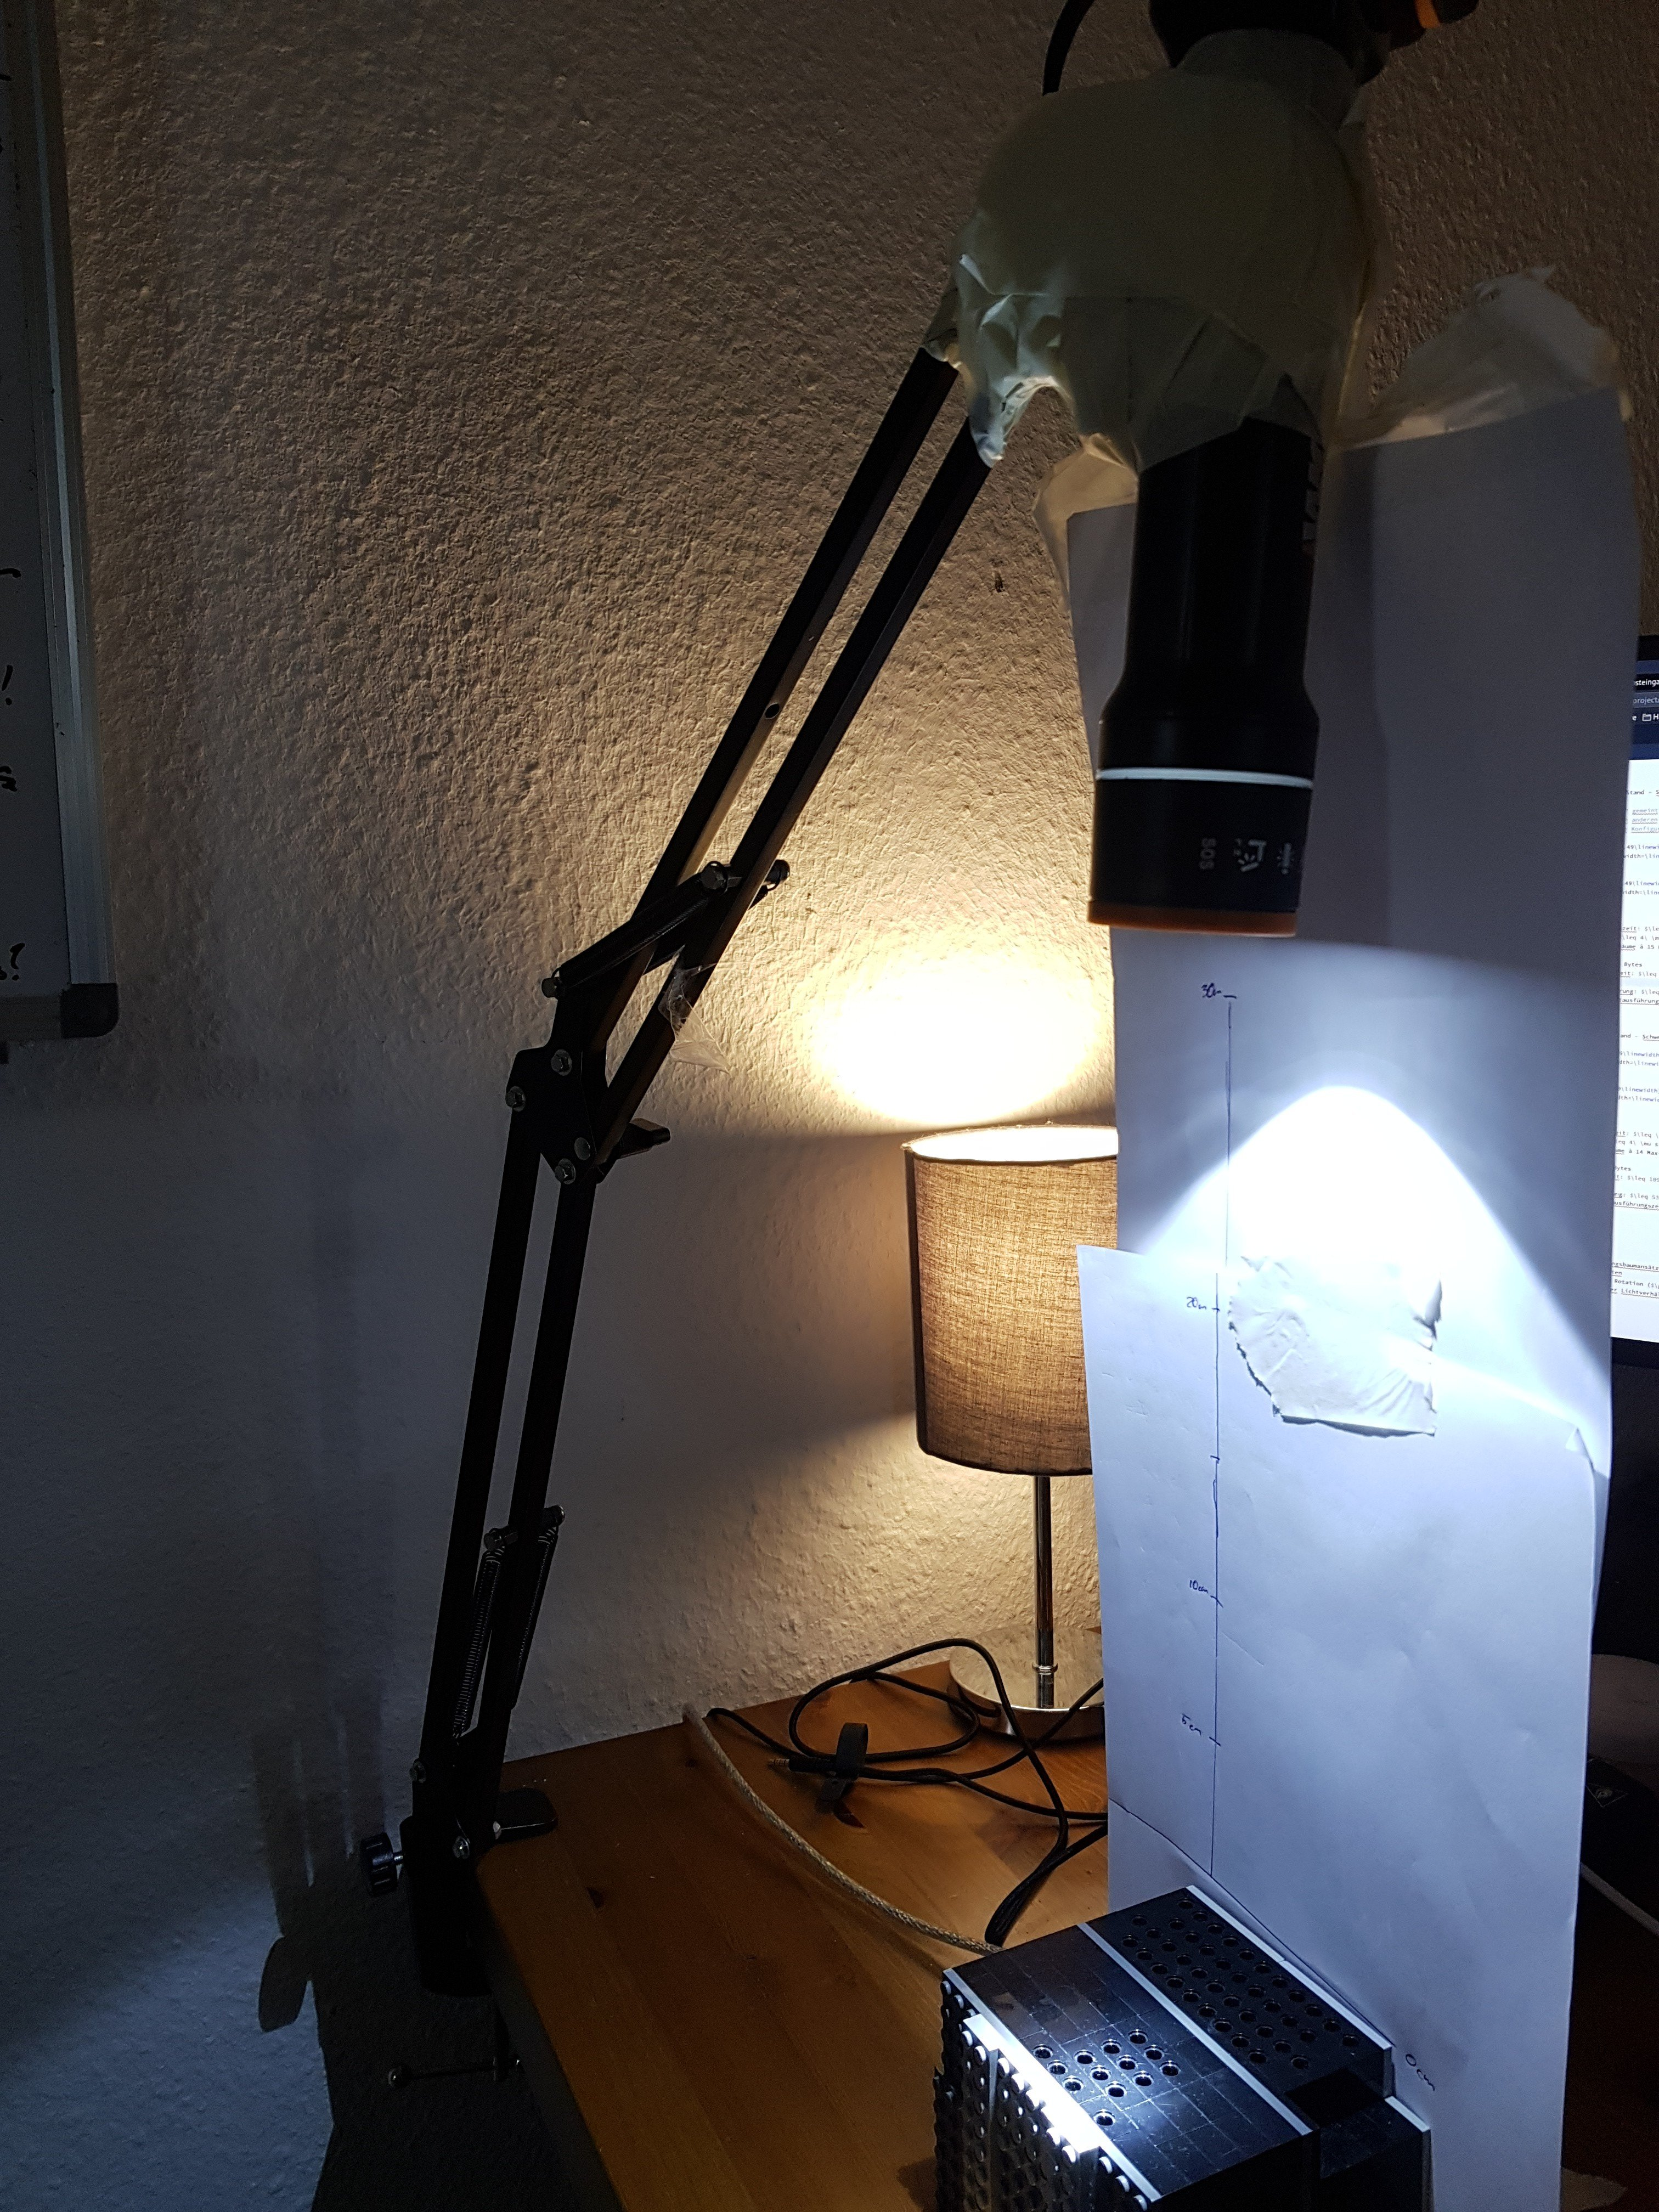
\includegraphics[width=0.33\linewidth]{images/light_high.jpeg}}%
}{Verschiedene Helligkeitsstufen unter denen die Gesten von \texttt{DymelData} aufgenommen wurden.}{fig:different_lights}
Jede Handgeste wurde unter jeder Konfiguration ca. 100 mal aufgenommen bei 90 Bildern pro Sekunde. Insgesamt wurden in 3 Lichtverhältnisse und 4 Distanzen, 6 verschiedene Gesten (Links nach Rechts,
Rechts nach Links, Oben nach Unten, Unten nach Oben und 2 Nullgesten) jeweils schnell und langsam aufgenommen. Die Gesten wurden in den Abständen 5 cm, 10 cm, 20 cm und 25 cm aufgenommen.
\newline
\newline
Die \glqq Geringe\grqq\ Helligkeit war im Durchschnitt bei ca. 140, \glqq Halbe\grqq\ Helligkeit bei ca. 659, \glqq Hohe\grqq\ Helligkeit bei ca. 908. Alle Helligkeiten haben das 3x3-Array
relativ gleichmäßig ausgeleuchtet. Bei den Lichtquellen \ref{subfig:light_low} und \ref{subfig:light_medium} wurde eine Schirmlampe verwendendet. Dadurch wurde das Licht relativ breit gestreut,
wodurch der Kontrast mit vergrößender Distanz abgenommen hat. Bei \ref{subfig:light_high} wurde eine Punktlichtquelle verwendet, wodurch der Kontrast über alle Distanzen sehr stark ist.
\newline
\newline
Insgesamt wurden 2 Typen von Nullgesten aufgenommen. Die erste Nullgeste geht \textit{Oben} rein, verschieden weit in Richtung \textit{Unten} und kehrt anschließend um, um bei \textit{Oben} wieder rauszukommen.
Die zweite Nullgeste geht \textit{Oben} rein, verschieden weit in Richtung \textit{Unten} und anschließend \textit{Rechts} wieder raus.
\newline
\newline
Die resultierenden Handgesten werden anschließend um 90°, 180° und 270° rotiert, um die equivalenten Nullgesten aus den anderen Richtungen zu inferieren. Insgesamt enstehen dadurch 19400 Nullgesten.
\newline
\newline
Um zu testen wie gut das Model sich gegenüber verschiedene Lichtverhältnisse generalisiert hat, ist es nötig mehr als nur 3 Helligkeitsstufen zu testen. Aus diesem Grund wurde aus der Gestenmenge mit
der Helligkeit \glqq Gering\grqq\ eine synthetische Testmenge generiert.
\newline
\newline
Dabei wurden jeweils 20 Duplikate der Datenmenge erstellt mit einem Helligkeitsoffset zwischen 50 und 1000 und einer Skalierung zwischen 0,5 und 10. Diese Datenmengen wurden zu einer Testmenge zusammengefügt.
\section{Features}
Features bilden die Eingabe für einen Entscheidungsbaum. Gute Features sind integral, damit der Entscheidungsbaum gut generalisiert. Wenn die Featuremenge keine eindeutige Trennung der Klassen in der
Trainingsmenge zulässt, so ist auch keine gute Generalisierung zu erwarten.
\newline
\newline
In dieser Arbeit muss die Richtung der Handgeste klassifiziert werden. Die Handgeste kann mit verschiedenen Geschwindigkeiten und unterschiedlichen Distanzen zur Kamera durchgeführt werden. Mit
zunehmender Entfernung nimmt der Kontrast ab, da Streulicht einen größeren Einfluss hat. Für eine gute Generalisierung sollten die Features Invarianten zur Geschwindigkeit und den
Lichtverhältnissen haben. Erschwerend ist, dass die Handgeste nie exakt gleich ausgeführt wird. Sie kann leichte Kreisbewegungen aufweisen oder schräg durchgeführt werden, sodass einige
Fotowiderstände nicht verdeckt werden.
\subsection{Feature Verbesserungen}
Einige Anforderungen, können durch spezielle Änderungen an einem Feature ergänzt werden. Dazu gehören relative Helligkeitsunterschiede, Positionsinformationen und Entwicklung über die Zeit.
\newline
\newline
Relative Helligkeitsunterschiede können durch Normalisierung über die lokale Gesamthelligkeit eliminiert werden. Dadurch ändert sich aber die Art der Aussage über die absolute Helligkeit
zu einer Aussage über die relative Helligkeit. Das heißt, jeder Pixel in einem Bild wird durch die Summe der Pixel im Bild geteilt. Dies erzeugt eine Invarianz gegenüber der skalierten Helligkeiten,
jedoch nicht gegenüber Helligkeiten auf denen ein Offset addiert wurde.
\newline
\newline
Informationen über die Position können einerseits aus dem Argument des Features und andererseits durch partielle Anwendung inferiert werden. Beim Argument eines Features wird das Argument als Feature
bereitgestellt, indem das Feature bestimmte Bedingungen erfüllt. Bei $\arg(\max X)$ zum Beispiel, wird der Index bereitgestellt, an dem die Menge $X$ maximal ist. Bei der partiellen Anwendung wird das Feature auf
Teilmengen der Definitionsmenge angewendet und damit mehrfach zur Feature-Menge hinzugefügt, z. B. bei der Fotowiderstandmatrix könnten Zeilen und Spalten Teilmengen sein.
\newline
\newline
Die Entwicklung über Zeit kann ebenfalls über die Duplizierung des Features dargestellt werden. Anstatt einen einzelnen Bild zu unterteilen, wird die Handgeste in Zeitfenster aufgeteilt. Jedes Zeitfenster
fasst die einzelnen Bilder zu einem Bild zusammen. Für jedes Zeitfenster wird das Feature berechnet.
\subsection{Featureauswahl}
Insgesamt wurden 28 Varianten von Feature untersucht und davon 3 Feature verstärkt aus denen 20 Varianten entstanden sind. Die Features, die von Song et al. genutzt wurden
(siehe Tabelle \ref{tab:songFeatures}) eignen sich ohne Änderungen nicht, da sie mindestens eine Anforderung nicht erfüllen.
\newline
\newline
Mit dem \textit{Mean absolute value} ermöglicht es die einzelnen Handgesten zu unterscheiden, wenn das Feature in verschiedene Zeitfenster aufgeteil wird. Zusätzlich kann die Helligkeit normalisiert werden.
Um die Featuremenge zu verringern, können Spalten und Zeilen zusammengefasst werden. Allerdings generalisierte der Ansatz nicht gut, da die Varianz sehr groß ist durch die fehlende Invarianz zur Geschwindigkeit.
\newline
\newline
\textit{Average amplitude change} eignet sich gut um horizontale und vertikale Bewegungen zu unterscheiden. Allerdings ist es nicht möglich symethrische Bewegungen zu unterscheiden. Nicht untersucht wurden
Änderungen, die beim \textit{Mean absolute value} durchgeführt wurden.
\newline
\newline
Feature 2, 5, 7 bis 9 wurden nicht weiter untersucht weil sie zu komplexe Berechnungen bedürfen für das Arduino Board.

\subsubsection{Motion History}
Die Motion History zeigt eine Bewegunghistorie, indem kürzlich stattgefundene Bewegung heller ist als länger zurückliegende. Es ist invariant gegenüber Lichtverhältnisse, hat jedoch 2 große Schwachpunkte.
Einerseits kann es überlappende Bewegungen nicht richtig anzeigen, da eine kürzlich detektierte Bewegungung den Wert auf den Maximalwert $\tau$ setzt. Dies stellt in diesem Anwendungsfall kein
Problem dar, da die definierten Handgesten keine Überlappung erzeugen.
\newline
\newline
Andereseits ist das Feature bei konstantem $\tau$ und $\delta$ nicht Invariant gegenüber Geschwindigkeit. Als Lösung wurde $\delta$ abhängig von der Gestenlänge gemacht,
d. h. $\delta = \frac{\tau}{\#Bilder}$. Mit dieser Konfiguration ist die Bewegung nicht unvollständig, wenn sie langsam ausgeführt wird. Allerdings geht dieser Ansatz von einer konstanten
Ausführungsgeschwindigkeit der Handgeste aus.
\newline
\newline
Eine Bewegung in einem Pixel $q$ wird duch die Funktion \ref{formular:motion_history_phi} signalisiert, d. h. die Bewegung in $q$ findet statt, wenn eine Veränderung oberhalb des Durchschnitts detektiert wird.
\begin{align}
    \phi(q,t) = \begin{cases}
                    1 & if \Delta_{q,t} \geq \frac{1}{N} \sum_{n=1}^N \Delta_{q,n} \\
                    0 & otherwise
    \end{cases}
    \hspace{0.5cm}where\ \Delta_{q,t} = |q_t - q_{t-1}|
    \label{formular:motion_history_phi}
\end{align}

\subsubsection{Helligkeitsverteilung}
Ein Pixel $q$ ist am hellsten unter allen Pixeln in einem Bild $Q$, wenn $q$ den höchsten Wert hat. Analog ist der dunkelste Pixel, der mit dem geringsten Wert. Folglich kann der hellste Pixel als
$q' = \arg(\max Q)$, bzw. der dunkelste Pixel als $q' = \arg(\min Q)$ definiert werden.
\newline
\newline
Weiterhin wird die Bildsequenz in eine bestimmte Anzahl von gleich großen Zeitfenstern aufgeteilt. In jedem Zeitfenster wird der hellste bzw. dunkelste Pixel ermittelt. Aus der daraus resultierenden
Featuremenge kann jede definierte Handgeste inferiert werden. Sie ist invariant zu Lichtverhältnissen und Geschwindigkeiten. Per Definition gibt sie Auskunft über die Entwicklung über Zeit und die Position.
\newline
\newline
Es gibt mehrere Möglichkeiten die einzelnen Pixel in einem Zeitfenster zusammenzufassen.
\begin{itemize}
    \item Wähle das Minimum bzw. Maximum.
    \item Projeziere die Pixel auf ein kartesisches Koordinatensystem und fasse die Punkte über eine Abstandsmetrik zusammen, z. B. über den euklidischen Abstand.
    \item Unterteile die Pixel in Quadranten und wähle den Quadranten, der die meisten Einträge hat.
\end{itemize}
Außerdem können die Anzahl der Zeitfenster variiert werden und Pixel zu Gruppen zusammengefasst werden, d. h. Spalten und Zeilen.

\subsubsection{Schwerpunktverteilung}
\begin{figure}
    \centering
    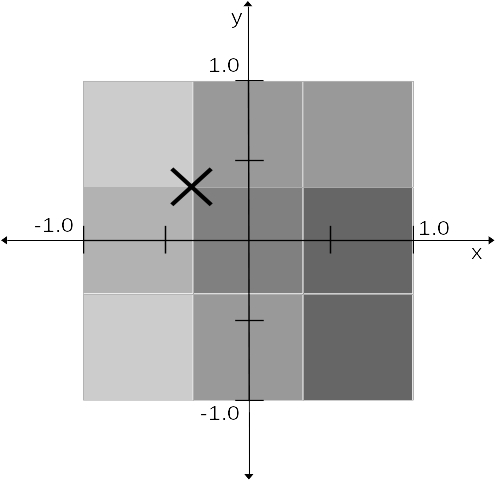
\includegraphics[width=0.5\linewidth]{images/schwerpunkt_ansatz.jpg}
    \caption{Illustration des Schwerpunktes im 3x3 Fotowiderstand-Array.}
    \label{fig:schwerpunkt}
\end{figure}
\begin{align}
    Q = \begin{pmatrix}
            q_{00} & q_{01} & q_{02} \\
            q_{10} & q_{11} & q_{12} \\
            q_{20} & q_{21} & q_{22}
    \end{pmatrix}
    \label{formular:pictureAsFormular}
\end{align}
Der Schwerpunkt $(X_Q, Y_Q)$ in einem Bild $Q$ (\ref{formular:pictureAsFormular}) ist über die Helligkeit in den einzelnen Pixel definiert. Der Pixel $q_{11}$ bildet den Nullpunkt des Koordinatensystems.
Dann ist relativ zur Gesamthelligkeit $P = \sum_{i,j} q_{i,j}$, $X_Q=\frac{\sum_{i=0}^{2} q_{i,2} - \sum_{i=0}^{2} q_{i,0}}{P}$ die horizontale Komponente
und $Y_Q = \frac{\sum_{i=0}^{2} q_{0,i} - \sum_{i=0}^{2} q_{2,i}}{P}$ die vertikale Komponente des Schwerpunktes \cite{schwerpunktAnsatz}.
\newline
\newline
Ähnlich zur Helligkeitsverteilung wird das Feature mit einer Zeithistorie erweitert durch die multiple Anwendung auf verschiedene Zeitfenster, wobei die Anzahl der Zeitfenster variiert werden kann. Die
einzelnen Schwerpunkte innerhalb eines Zeitfensters werden über den Durchschnitt zusammengefasst.
\newline
\newline
Sollte die Anzahl der Bilder einer Handgeste ein Vielfaches von der Anzahl der Zeitfenster sein, wird die gleiche Anzahl an Bilder auf jedes Zeitfenster verteilt. Ansonsten werden Überschüsse einem Muster
nach bestimmten Zeitfenstern zugeordnet. Bei 5 Zeitfenstern wird der erste Überschuss dem letzten Zeitfenster zugeordnet, der zweite dem ersten, der dritte dem dritten, der vierte dem zweiten.
\newline
\newline
Die Schwerpunktverteilung ist durch die Dividierung mit $P$ invariant gegenüber Skalierung der Helligkeit, jedoch nicht gegenüber einen Offset.

\section{Klassifizierungsgenauigkeit}
Es werden drei Features näher betrachtet. Motion History, Helligkeitsverteilung und Schwerpunktverteilung. Daraus wurden vier Feature-Mengen generiert, die zum Trainieren genutzt werden. Insgesamt wurden 22528
verschiedene Konfigurationen trainiert und getestet, die in Kapitel \ref{sec:Training} beschrieben wurden. Jede Konfiguration nutzt zum Trainieren eine Kombination aus der Trainingsmenge von Feng und Kubik,
sowie die Gestentestmenge und die Nullgestenmenge, die in Kapitel \ref{sec:DymelData} beschrieben wurden. Die Trainingsmenge beinhaltet insgesamt 7629 Handgesten. Davon wird 50\% zum Trainieren und 50\% zum
Validieren und Optimieren auf Basis der Monte Carlo Methode benutzt.
\newline
\newline
Unter jeder Feature-Menge werden jeweils drei Kategorien analysiert. Die erste Kategorie zeigt die beste Konfiguration, die ohne Restriktion des Programmspeichers gefunden wurde. Die zweite Kategorie hat eine Restriktion
von 48 kB und die dritte Kategorie hat eine Restriktion von 32 kB. Diese beziehen sich auf den Programmspeicher des ATmega4809 und ATmega328P, die im Rahmen der Fallstudie verwendet werden \cite{venzkeArticle}.
Dabei werden immer 4 kB abgezogen, da diese für andere systemrelevante Funktionen reserviert sind. Die beste Konfiguration einer Kategorie maximiert die Summe
der Klassifizierungsgenauigkeiten der Testmenge von Klisch, der Gestentestmenge und der Nullgestentestmenge. Dabei wird stets die optimierte Programmgröße der Konfiguration betrachtet, nachdem alle Optimierungen aus Kapitel
\ref{sec:eval_size} angewendet wurden.
\newline
\newline
In der Analyse werden die verschiedenen Feature-Mengen im Hinblick auf die Klassifizierungsgenauigkeit der Testmenge von Klisch, der Gestentestmenge, der Nullgestentestmenge und den synthetischen
Helligkeitstestmengen untereinander verglichen und mit den Ergebnissen von Giese verglichen. Es wird ausschließlich mit Giese verglichen, da seine Ergebnisse die beste Klassifizierungsgenauigkeit,
geringste Ausführungszeit und geringsten Ressourcenverbrauch erzielte. Außerdem wird die Auswirkung von verschiedenen Waldgrößen auf die Klassifizierungsgenauigkeit untersucht. Anzumerken ist, dass
lediglich die Testmenge von Klisch vergleichbar mit den Ergebnissen von Giese ist, da die Gestentestmenge, Nullgestentestmenge und Helligkeitstestmengen erst im Laufe dieser Arbeit entstanden sind.

\subsection{Helligkeitsverteilung}
\begin{table}[h!]
    \centering
    \begin{tabular}{ | l | c | c | c |}
        \hline
        Konfiguration & Beste & Unter 44 kB & Unter 28 kB \\\hline
        Ensemble-Methode & ExtraTrees & ExtraTrees & ExtraTrees \\\hline
        Maximalhöhe & 14 & 10 & 15 \\\hline
        Waldgröße & 10 & 6 & 1 \\\hline
        Blattgröße (min\_samples\_leaf) & 4 & 4 & 4 \\\hline
        Programmgröße in Bytes & 76628 & 33284 & 9364 \\\hline
        Genauigkeit Testmenge von Klisch & 74,0\% & 63,5\% & 67,7\% \\\hline
        Genauigkeit Gestentestmenge & 74,1\% & 79,2\% & 76,6\% \\\hline
        Genauigkeit Nullgestentestmenge & 69,0\% & 71,0\% & 67,0\% \\\hline
    \end{tabular}
    \caption{Die beste Konfigurationen der Helligkeitsverteilung.}
    \label{tab:helligkeitsverteilung}
\end{table}
\begin{figure}[h!]
    \centering
    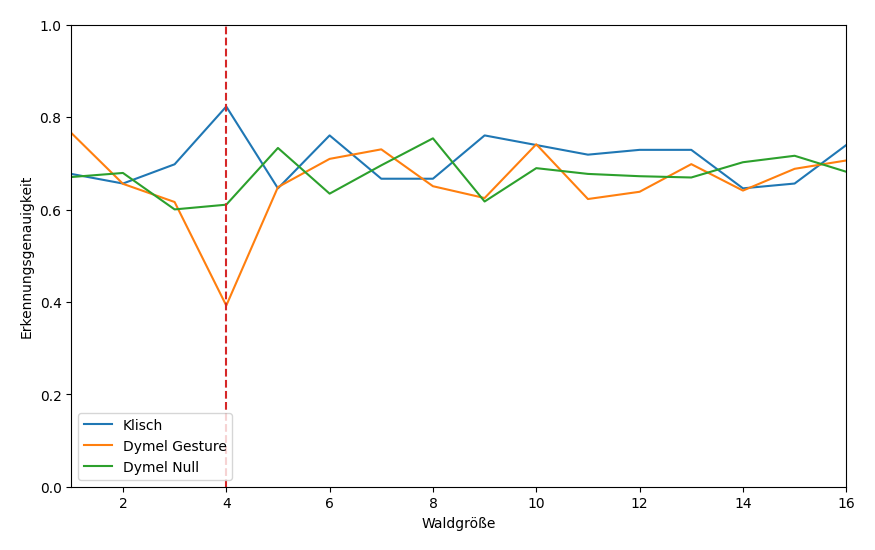
\includegraphics[width=\linewidth]{images/helligkeitsverteilung_acc_per_size.png}
    \caption{Die besten Konfigurationen pro Waldgröße mit der Helligkeitsverteilung.}
    \label{fig:helligkeitsverteilung_per_forest_size}
\end{figure}
Die Featuremenge der Helligkeitsverteilung beinhaltet insgesamt 12 Features. Jeweils 6 Feature repräsentieren Zeitfenster der minimalen Helligkeit und der maximalen Helligkeit. Die Zeitfenster wurden
geometrisch zusammengefasst.
\newline
\newline
Aus der Tabelle \ref{tab:helligkeitsverteilung} sind die besten Konfigurationen jeder Kategorie zu entnehmen. Die beste Konfiguration wurde mit der Ensemble-Methode \textit{ExtraTrees} gefunden.
Sie erzielt eine Klassifizierungsgenauigkeit von 74\% auf der Testmenge von Klisch und ist damit 25,2\% schlechter als das neuronale Netzwerk von Giese \cite{gieseThesis}. Außerdem wird 74\% der Gestentestmenge
und 69\% der Nullgestentestmenge korrekt klassifiziert.
\newline
\newline
Wird die Kategorie \textit{Beste} und die Kategorie \textit{Unter 28 kB} vergleichen, nimmt die Gesamtklassifizierungsgenauigkeit nur um 1,94\% ab. Dabei reduziert sich die Programmgröße um 87,8\%.
Ein ähnliches Verhalten ist auch in Abbildung \ref{fig:helligkeitsverteilung_per_forest_size} zu erkennen. Dort ist nur ein geringer Zuwachs der Gesamtklassifizierungsgenauigkeit mit der zunehmenden
Waldgröße zu beobachten.
\subsection{Motion History}
\begin{table}[h!]
    \centering
    \begin{tabular}{ | l | c | c | c |}
        \hline
        Konfiguration & Beste & Unter 44 kB & Unter 28 kB \\\hline
        Ensemble-Methode & ExtraTrees & ExtraTrees & ExtraTrees \\\hline
        Maximalhöhe & 10 & 11 & 9 \\\hline
        Waldgröße & 16 & 7 & 6 \\\hline
        Blattgröße (min\_samples\_leaf) & 1 & 2 & 1 \\\hline
        Programmgröße in Bytes & 84200 & 40456 & 22804 \\\hline
        Genauigkeit Testmenge von Klisch & 68,8\% & 67,7\% & 62,5\% \\\hline
        Genauigkeit Gestentestmenge & 74,5\% & 67,6\% & 68,5\% \\\hline
        Genauigkeit Nullgestentestmenge & 68,3\% & 64,4\% & 67,6\% \\\hline
    \end{tabular}
    \caption{Die besten Konfigurationen der Feature-Menge Motion History.}
    \label{tab:motion_history}
\end{table}
\begin{figure}[h!]
    \centering
    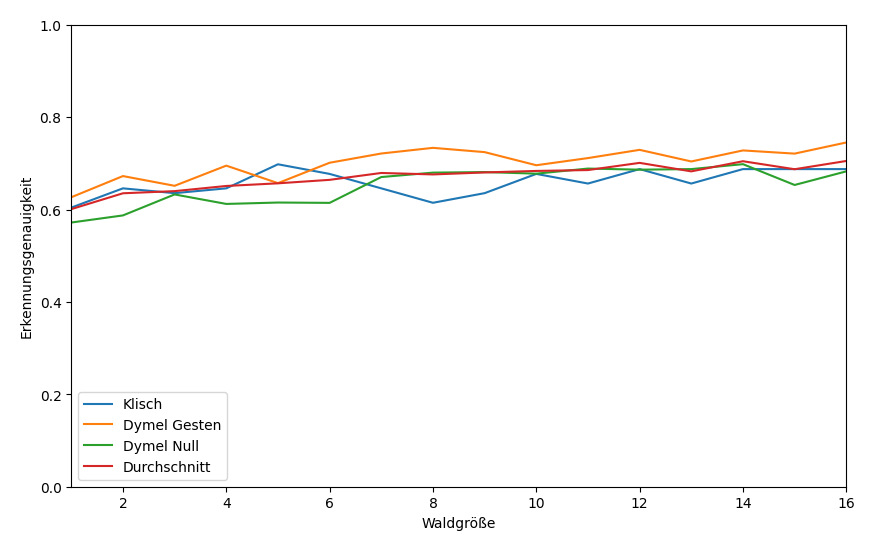
\includegraphics[width=\linewidth]{images/motion_history_acc_per_size.png}
    \caption{Die besten Modelle pro Waldgröße der Feature-Menge Motion History.}
    \label{fig:motion_history_per_forest_size}
\end{figure}
Die Feature-Menge Motion History beinhaltet für jeden Pixel ein Feature, das der Definition des Motion History Image folgt (Formel \ref{formular:mhi}), wobei $\tau=100$ und $\delta=\frac{\tau}{\#Bilder}$ ist.
\newline
\newline
Aus Tabelle \ref{tab:helligkeitsverteilung} sind die besten Konfigurationen jeder Kategorie zu entnehmen. Die beste Konfiguration wurde wieder mit der Ensemble-Methode \textit{ExtraTrees} gefunden.
Das Modell erzielt eine Klassifizierungsgenauigkeit von 68,8\% auf der Testmenge von Klisch, 74\% auf der Gestentestmenge und 69\% auf der Nullgestentestmenge. Im Vergleich zu der Helligkeitsverteilung
wird mehr Programmspeicher benötigt und die Gesamtklassifizierungsgenauigkeit ist 1,84\% schlechter.
\newline
\newline
Wird die Kategorie \textit{Beste} mit der Kategorie \textit{Unter 28~kB} verglichen, nimmt die Gesamtklassifizierungsgenauigkeit nur um 4,3\% ab. Dabei reduziert sich die Programmgröße um 72,9\%.
Abbildung \ref{fig:motion_history_per_forest_size} zeigt, dass die Klassifizierungsgenauigkeit im Durchschnitt sich mit zunehmender Waldgröße erhöht. Im Vergleich zur Helligkeitsverteilung, ist der Zuwachs größer.
Wenn der Suchraum nicht auf eine Waldgröße von 16~Bäumen begrenzt wäre, würde die beste Konfiguration vermutlich besser sein. Allerdings würde sich auch die Programmgröße signifikant erhöhen.
\newline
\newline
Die Motion History kann mit ausschließlich 8-Bit Integer implementiert werden und hat damit die geringste WCET und Programmgröße pro Baum, weswegen die beste Konfiguration mit einer Waldgröße von 16~Bäumen nicht deutlich
größer ist, als die der Helligkeitsverteilung mit einer Waldgröße von 10~Bäumen.

\subsection{Schwerpunktverteilung mit Gleitkommazahlen}
\begin{table}[h!]
    \hspace{-0.5cm}
    \begin{tabular}{ | l | c | c | c | c |}
        \hline
        Konfiguration & Beste & Unter 60 kB & Unter 28 kB & Unter 14 kB \\\hline
        Ensemble-Methode & Boosting & Boosting & RandomForest & Bagging  \\\hline
        Maximalhöhe & 20 & 19 & 10 & 7 \\\hline
        Waldgröße & 10 & 6 & 4 & 3 \\\hline
        min\_samples\_leaf & 8 & 8 & 2 & 8 \\\hline
        Programmgröße in Bytes & 83304 & 43678 & 20188 & 6656 \\\hline
        Genauigkeit Testmenge von Klisch & 94,8\% & 94.8\% & 89,6\% & 87,5\% \\\hline
        Genauigkeit Gestentestmenge & 97,0\% & 96,1\% & 95,6\% & 94,1\% \\\hline
        Genauigkeit Nullgestentestmenge & 92,2\% & 91,1\% & 88,8\% & 89,9\% \\\hline
    \end{tabular}
    \caption{Beste Konfigurationen der Schwerpunktverteilung mit Gleitkommazahlen.}
    \label{tab:schwerpunktverteilung_float}
\end{table}
\begin{figure}[h!]
    \centering
    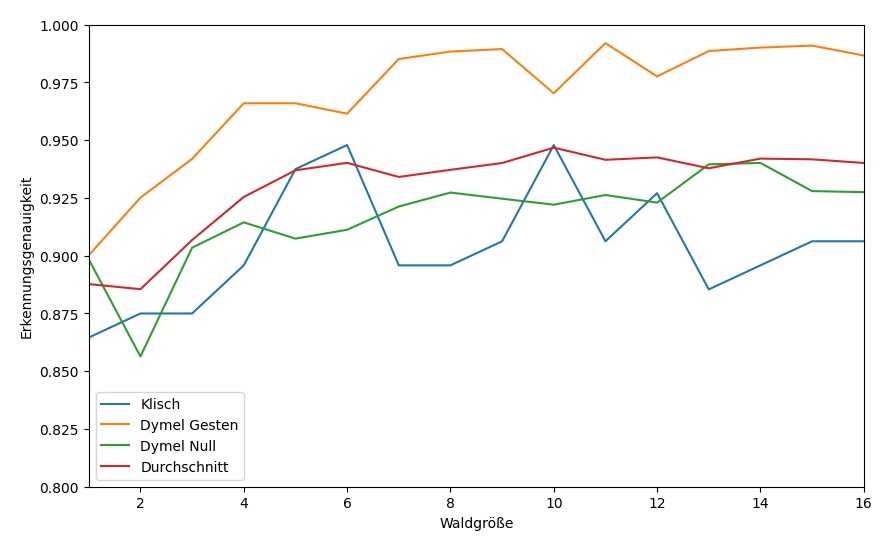
\includegraphics[width=\linewidth]{images/cocd_float_acc_per_size.png}
    \caption{Die beste summierte Erkennungsgenauigkeit pro Waldgröße der Schwerpunktverteilung mit Gleitkommazahlen.}
    \label{fig:cocd_float_per_forest_size}
\end{figure}
Die Featuremenge Schwerpunktverteilung mit Gleitkommazahlen folgt der Definition aus Sektion \ref{sec:schwerpunktverteilung} und beinhaltet insgesamt 10 Einträge, wobei jeweils 2 Einträge die X und Y
Koordinate des Schwerpunktes darstellen in insgesamt 5 Zeitfenstern.
\newline
\newline
Die beste Konfiguration wurde mit der Ensemble-Methode Boosting erzielt (siehe Tabelle \ref{tab:schwerpunktverteilung_float}). Mit einer Erkennungsgenauigkeit von 94,8\% auf der Testmenge von Klisch
ist dieser Ansatz nur 5,2\% schlechter als das neuronale Netz von Giese \cite{gieseThesis}. Es ist anzumerken, dass mit einer kleineren Trainingsmenge ohne die Gestentrainingsmenge und Nullgestentrainingsmenge eine Lösung
gefunden wurde, die 97,9\% erzielte und damit nur 2,1\% schlechter ist. Außerdem werden 97\% der Gestentestmenge und 92,2\% der Nullgestentestmenge korrekt klassifiziert.
\newline
\newline
Im Vergleich zu der Helligkeitsverteilung und Motion History ist die Erkennungsgenauigkeit dieses Ansatzes signifikant besser, sogar wenn nur 6656 Byte Programmspeicher verwendet werden. Wird die beste Konfiguration mit
der \textit{Unter 14 kB} verglichen, nimmt die Gesamterkennungsganuigkeit nur um 4,17\% ab bei der Reduktion der Programmgröße von 92\%. Dies verspricht, dass mit zunehmender Waldgröße der die Erkennungsgenauigkeit steigt.
Abbildung \ref{fig:cocd_float_per_forest_size} zeigt, dass dies zwar der Fall ist, aber schon ab einer Waldgröße von 6 ist die Durchschnittliche Erkennungsgenauigkeit keinen signifikanten Zuwachs mehr verzeichnet.
Dementsprechend ist der Unterschied der Gesamterkennungsgenauigkeit der besten Konfiguraiton und \textit{Unter 60 kB} mit 0,7\% nicht groß, wodurch sich dieses Feature gut für kleine eingebettete Systeme mit
wenig Programmspeicher eignet.
\subsection{Schwerpunktverteilung mit Ganzzahlen}
\begin{table}[h!]
    \hspace{-0.5cm}
    \begin{tabular}{ | l | c | c | c |}
        \hline
        Konfiguration & Beste & Unter 44 kB \& 28 kB & Unter 14 kB \\\hline
        Ensemble-Methode & ExtraTrees & Random Forest & Random Forest \\\hline
        Maximalhöhe & 21 & 13 & 12 \\\hline
        Waldgröße & 11 & 7 & 3 \\\hline
        Blattgröße (min\_samples\_leaf) & 2 & 4 & 1 \\\hline
        Programmgröße in Bytes & 76200 & 21532 & 11012 \\\hline
        Genauigkeit Testmenge von Klisch & 95,8\% & 91,7\% & 86,5\% \\\hline
        Genauigkeit Gestentestmenge & 98,8\% & 97,1\% & 95,5\% \\\hline
        Genauigkeit Nullgestentestmenge & 95,6\% & 94,5\% & 88,9\% \\\hline
    \end{tabular}
    \caption{Die besten Konfigurationen der Schwerpunktverteilung mit Ganzzahlen.}
    \label{tab:schwerpunktverteilung_int}
\end{table}
\begin{figure}[h!]
    \centering
    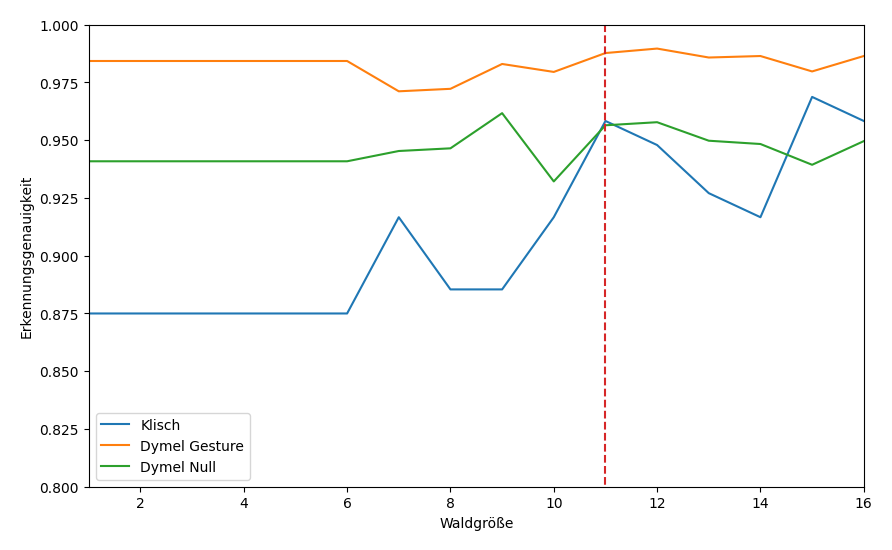
\includegraphics[width=\linewidth]{images/cocd_int_acc_per_size.png}
    \caption{Die besten Konfigurationen pro Waldgröße der Schwerpunktverteilung mit Ganzzahlen.}
    \label{fig:cocd_int_per_forest_size}
\end{figure}
Die Featuremenge Schwerpunktverteilung mit Ganzzahlen folgt der Definition aus Kapitel \ref{sec:schwerpunktverteilung} und beinhaltet insgesamt 10 Einträge. Jeweils 2 Einträge bilden die X und Y
Koordinate des Schwerpunktes. Damit spiegeln 10 Einträge insgesamt 5 Zeitfenster wieder.
\newline
\newline
Aus der Tabelle \ref{tab:schwerpunktverteilung_int} sind die besten Konfigurationen jeder Kategorie zu entnehmen. Die beste Konfiguration wurde mit der Ensemble-Methode ExtraTrees gefunden.
Mit einer Klassifizierungsgenauigkeit von 95,8\% auf der Testmenge von Klisch ist dieser Ansatz nur 3,2\% schlechter als das neuronale Netz von Giese \cite{gieseThesis}. Es wurde aber auch eine Konfiguration
gefunden, die 96,9\% der Testmenge von Klisch korrekt klassifiziert und damit nur 2,1\% schlechter ist. Diese maximiert aber in keiner Kategorie die Gesamtklassifizierungsgenauigkeit.
Außerdem werden 98,8\% der Gestentestmenge und 95,6\% der Nullgestentestmenge korrekt klassifiziert. Es wurde kein Entscheidungswald gefunden, der weniger als 44 kB Programmspeicher benötigt und besser ist als die
Konfiguration in der Kategorie \textit{Unter 28 kB}.
\newline
\newline
Der Ansatz mit Ganzzahlen erzielte eine 2,1\% höhere Gesamtklassifizierungsgenauigkeit als der Ansatz mit Gleitkommazahlen. Der 16-Bit Integer Datentyp erlaubt der Schwerpunktverteilung mit Ganzzahlen unter jeder
Restriktion größere Entscheidungswälder zu bilden, als die Schwerpunktverteilung mit Gleitkommazahlen. Abbildung \ref{fig:cocd_int_per_forest_size} zeigt einen Zuwachs der durchschnittlichen Klassifizierungsgenauigkeit
mit zunehmender Waldgröße. Es ist auszugehen, dass eine noch bessere Konfiguration gefunden werden könnte, wenn der Suchraum auf eine größere Waldgröße erweitert wird. Ähnlich wie die Schwerpunktverteilung mit
Gleitkommazahlen ist der Zuwachs der durchschnittlichen Klassifizierungsgenauigkeit ab einer Waldgröße von 7 Bäumen gering. Somit kann bereits bei einer geringen Programmgröße eine hohe Klassifizierungsgenauigkeit
erzielt werden. Damit eignet sich die Schwerpunktverteilung mit Ganzzahlen ebenfalls für kleine eingebettete Systeme.

\subsection{Kombinierte Schwerpunktverteilung}
\begin{table}[h!]
    \centering
    \begin{tabular}{ | l | c | c | c | c |}
        \hline
        Konfiguration & Beste & Unter 44 kB & Unter 28 kB \\\hline
        Schwerpunktverteilung Gleitkommazahl & Beste & Unter 14 kB & Unter 14 kB \\\hline
        Schwerpunktverteilung Ganzzahlen & Beste &  Unter 28 kB & Unter 14 kB \\\hline
        Programmgröße in Bytes & - & 33276 & 20252 \\\hline
        Genauigkeit Testmenge von Klisch & 94,8\% & 87,5\% & 87,5\% \\\hline
        Genauigkeit Gestentestmenge & 99,0\% & 97,7\% & 96,9\% \\\hline
        Genauigkeit Nullgestentestmenge & 95,8\% & 92,9\% & 92,5\% \\\hline
    \end{tabular}
    \caption{Die besten Konfigurationen der kombinierten Schwerpunktverteilung.}
    \label{tab:schwerpunktverteilung_int_and_float}
\end{table}
Die kombinierte Schwerpunktverteilung vereint die Schwerpunktverteilung mit Ganzzahlen und Gleitkommazahlen. Das erscheint sinnvoll, da der Ansatz mit Ganzzahlen invariant zu einem Offset in der
Helligkeit ist und der Ansatz mit Gleitkommazahlen invariant zur Skalierung der Helligkeit.
\newline
\newline
Es wird davon ausgegangen, dass der jeweilige Klassifizierer entweder ein Ergebnis mit einer deutlichen Mehrheit zurückgibt oder ein Ergebnis mit einer knappen Mehrheit. Für jedes Lichtverhältniss, hat mindestens ein
Klassifizierer eine deutliche Mehrheit. Damit erzielt die Kombination eine Mehrheit bei der korrekten Klasse. Die besten Konfigurationen der beiden Ansätze werden mit einem Wahlklassifizierer vereint.
Das heißt, die Wahrscheinlichkeitsverteilungen der Wahlklassifizierer der jeweiligen Ansätze werden zu gleichen Anteilen addiert.
\newline
\newline
Die Kombination der besten Konfigurationen beider Ansätze erzielt eine Klassifizierungsgenauigkeit von 94,8\% auf der Testmenge von Klisch. Dies entspricht der Klassifizierungsgenauigkeit der Schwerpunktverteilung mit
Gleitkommazahlen. 99\% der Gestentestmenge wird korrekt klassifiziert. Das ist besser als beide Ansätze. Die Nullgestestmenge wurde zu 95,8\% korrekt klassifiziert. Dies entspricht der Klassifizierungsgenauigkeit der
Schwerpunktverteilung mit Ganzzahlen. Bei der Kategorie \textit{Unter 44 kB} und \textit{Unter 28 kB} wurde der kombinierte Klassifizierer nie schlechter als der schlechteste Ansatz auf dem die kombinierte
Schwerpunktverteilung basiert.
\newline
\newline
Der Nachteil dieses Ansatzes ist, dass sowohl die Feature-Menge mit Gleitkommazahlen, als auch für Ganzzahlen benötigt wird. Zum einen müssen immer beide Features berechnet werden und zum anderen kann jeder Klassifizierer
nur halb so viel Speicher nutzen. Dadurch ist die Klassifizierungsgenauigkeit jedes Klassifizierers potenziell geringer, als wenn es den vollständigen Speicher zur Verfügung hätte. Bei der Schwerpunktverteilungen ist aber
bereits ab einer geringen Waldgröße kein signifikanter Zuwachs der Klassifizierungsgenauigkeit zu verzeichnen. Deswegen eignet sich die Schwerpunktverteilung besonders gut. Der Vorteil ist, dass der kombinierte
Klassifizierer potenziell robuster ist gegenüber unterschiedliche Lichtverhältnisse.


\subsection{Robustheit gegenüber Lichtverhältnisse}
TODO: For each best configuration per featureset add a line in the plot for scaling and offset invariance.


\section{Ausführungszeit}
\label{sec:eval_speed}
Die Ausführungszeit der Feature-Extrahierung und Klassifizierung ist ausschlaggebend für die mögliche FPS. Diese ermöglicht die Wahrnehmung von schnellen Handgesten. Ist die FPS bereits ausreichend
können leistungschwächere Module verwendet werden, wodurch die Batterielaufzeit verlängert wird oder die Kosten reduziert werden.
\newline
\newline
In dieser Arbeit wird das Arduino Board ATmega328P genutzt. Dieses Board verfügt über eine 8-Bit APU, 2 kB RAM, 32 kB Flash-Speicher und operiert unter 16 MHz \cite{atmega328p}.
Es verfügt nicht über ein Modul zur Verarbeitung von Gleitkommazahlen. Aus diesem Grund sind Operationen mit Gleitkommazahlen besonders teuer und zu vermeiden.
\newline
\newline
Es wird ausschließlich die \textit{Worst-Case-Execution-Time} (WCET) betrachtet. Ausschlaggebend dafür ist der \textit{Worst-Case-Execution-Path} (WCEP) im Kontrollflussgraph \cite{wcc_intro}. Der WCEP
setzt sich zusammen aus dem Vorgang das aktuelle Bild auszulesen, der Extrahierung der Features und der Ausführung des Klassifizierers.
\newline
\newline
Die Auswertung bezieht sich auf die Instruktionen des Programms, die bei der Übersetzung der Firmware durch den \textit{AVR GCC} mit der Optimierungsstufe \texttt{Os} entstehen. Aus dem Handbuch des
ATmega328P \cite{atmega328p} können für jede Instruktion die maximale Anzahl der Zyklen entnommen werden, die im schlimmsten Fall benötigt werden. Die Gesamtausführungszeit berechnet sich aus der Anzahl der Zyklen
multipliziert mit der Zeit pro Zyklus, d. h. bei 16 MHz bedarf ein Zyklus 0,0625 $\mu s$.

\subsection{Feature-Extrahierung}
Die Feature-Extrahierung implementiert die Berechnung der fünf Zeitfenster für die Schwerpunktverteilung. Einerseits muss aus jedem Bild der Schwerpunkt berechnet werden und andererseits müssen die Schwerpunkte
auf fünf Schwerpunkte zusammengefasst werden, die die fünf Zeitfenster repräsentieren.
\newline
\newline
Jedes Mal wenn ein Bild aufgenommen wird, wird der Schwerpunkt dieses Bildes berechnet und gespeichert. Dies reduziert einerseits die WCET, da im WCEP weniger Schwerpunkte berechnet werden müssen, und andererseits
wird weniger Pufferspeicher benötigt pro Bild. Für Gleitkommazahlen reduziert sich der Verbrauch pro Bild von 18 Byte auf 8 Byte und für Ganzzahlen auf 4 Byte. Der kombinierte Ansatz muss beide Schwerpunkte speichern.
Die jeweiligen Schwerpunktkoordinaten berechnen sich mit der in Kapitel \ref{sec:schwerpunktverteilung} beschriebenen Formel. Dabei muss die Summe der Pixel einmalig pro Bild berechnet werden und jeweils die
berechnete X und Y Koordinate im Puffer für den derzeitige Schwerpunkt gespeichert werden. Listing \ref{lst:cocdAlgoCOCDPerPicture} zeigt, wie dies auf dem ATmega328P implementiert ist. Insgesamt werden bei der
Schwerpunktverteilung mit Gleitkommazahlen 201 Zyklen für die einzelnen Instruktionen benötigt (12,5625 $\mu s$). Zusätzlich wird \textit{\_\_floatsisf} sechs mal aufgerufen, \textit{\_\_lesf2} und \textit{\_\_divsf3}
jeweils zwi mal aufgerufen. Die WCET zur Schwerpunktberechnung eines Bildes beläuft sich damit auf 116,5625 $\mu s$. Davon werden 104 $\mu s$ für Gleitkommaoperationen aufgewendet. Der Ansatz mit Ganzzahlen benötigt
keine Gleitkommaoperationen und 57 Zyklen weniger, da die summe der Pixel nicht berechnet werden muss, d. h. es werden für die WCET nur 8,875 $\mu s$ benötigt. Für den kombinierten Ansatz werden zusätzlich vier
Speicherinstruktionen benötigt, die einen Overhead von 0,25 $\mu s$ erzeugen, d. h. es werden für die WCET 116,8125 $\mu s$ benötigt.
\begin{lstlisting}[label=lst:cocdAlgoCOCDPerPicture,caption={Implementierung um den Schwerpunkt für ein Bild zu berechnen.}]
short helligkeits_summe = 0;
for (char i = 0; i < 9; ++i)
    helligkeits_summe += bild_puffer[i];
schwerpunkt_puffer_x[anzahl_bilder_im_puffer] = (float)(bild_puffer[0] + bild_puffer[3] + bild_puffer[6] - bild_puffer[2] - bild_puffer[5] - bild_puffer[8]) / ((float)helligkeits_summe);
schwerpunkt_puffer_y[anzahl_bilder_im_puffer] = (float)(bild_puffer[0] + bild_puffer[1] + bild_puffer[2] - bild_puffer[6] - bild_puffer[7] - bild_puffer[8]) / ((float)helligkeits_summe);
\end{lstlisting}
Wenn ein Handgestenkandidat detektiert wurde, wird für jedes Zeitfenster der Durchschnitt der darin enthaltenden Schwerpunkte berechnet. Die daraus berechneten Schwerpunkte werden als Schwerpunktverteilung bezeichnet.
Listing \ref{lst:cocdAlgo} zeigt den Algorithmus, um die Schwerpunktverteilung aus den Schwerpunkten im Puffer zu berechnen. Zunächst wird bei der Initialisierungsphase das \texttt{zusammenfass\_muster} berechnet
(Kap \ref{sec:schwerpunktverteilung}). Dafür werden im schlimmsten Fall 123 Zyklen für die einzelnen Instruktionen benötigt (7,6875 $\mu s$) und 20 $\mu s$ für die Ganzzahldividierung \textit{\_\_divmodhi4}. Insgesamt
27,6875 $\mu s$. Dieser Teil wird genau 1 mal für alle Richtungen und Schwerpunktverteilungen durchgeführt. Die innere Schleife wird im schlimmsten Fall für die Gesamtgröße des Schwerpunktpuffers durchlaufen.
Jeder Durchlauf benötigt im schlimmsten Fall 27 Zyklen für die einzelnen Instruktionen (1,6875 $\mu s$) und führt \textit{\_\_addsf3} einmal aus. Der WCET für einen Durchlauf beläuft sich damit auf 13,6875 $\mu s$.
Der Ansatz mit Ganzzahlen benötigt im schlimmsten Fall 17 Zyklen (1,125 $\mu s$). Bei einer Gesamtpuffergröße von 125 wird für den Teil der inneren Schleife für die Schwerpunktverteilung mit Gleitkommazahlen
1710,9375 $\mu s$ benötigt, für die Schwerpunktverteilung mit Ganzzahlen 140,625 $\mu s$ und für den kombinierten Ansatz 1851,5625 $\mu s$. Die äußere Schleife benötigt im schlimmsten Fall 57 Zyklen für die einzelnen
Instruktionen (3,5625 $\mu s$) und ruft im Ansatz mit Gleitkommazahlen fünf mal \textit{\_\_floatsisf} und \textit{\_\_divsf3} auf und im Ansatz mit Ganzzahlen fünf mal \textit{\_\_divmodhi4}. Damit beläuft sich der WCET
bei fünf Durchläufen der äußeren Schleife für den Ansatz mit Gleitkommazahlen auf 217,8125 $\mu s$, für den Ansatz mit Ganzzahlen auf 117,8125 $\mu s$ und für den kombinierten Ansatz 335,625 $\mu s$.
\begin{lstlisting}[label=lst:cocdAlgo,caption={Algorithmus um die Schwerpunktverteilung in horizontaler Richtung zu berechnen.}]
Initialisierung.
for (char i = 0; i < 5; ++i) { // Äußere Schleife
    features[i] = 0;
    for (char j = 0; j < zusammenfass_muster[i]; ++j) // Innere Schleife
        features[i] += *(schwerpunkt_puffer_x++);
    features[i] /= ((float)zusammenfass_muster[i]);
}
\end{lstlisting}
Der Schwerpunkt wird jeweils für die horizontale und vertikale Richtung berechnet. Der kombinierte Ansatz berechnet sowohl den Schwerpunkt für Gleitkommazahlen als auch für Ganzzahlen. Die WCET für die Feature-Extrahierung
der Schwerpunktverteilung mit Gleitkommazahlen beläuft sich auf 4001,75 $\mu s\ \approx\ $ 4 ms. Die WCET der Schwerpunktverteilung mit Ganzzahlen beläuft sich auf 553,4375 $\mu s\ \approx\ $ 0,6 ms. Die WCET der kombinierten
Schwerpunktverteilung beläuft sich auf 4518,875 $\mu s\ \approx\ $ 4,5 ms.

\subsection{Tree Evaluation}
\subsection{Ausführung eines Entscheidungswaldes}
Der WCEP eines Entscheidungswaldes setzt sich aus dem WCEP des Wahlklassifizierungsalgorithmus und dem WCEP jedes Entscheidungsbaumes zusammen, der im Wald enthalten ist.
\newline
\newline
Der in Listing \ref{lst:sklearnCCodeTreeVoting} gezeigte Code implementiert den Wahlvorgang. Die Komplexität ist abhängig von der Anzahl der Features $N$ und der Anzahl der Entscheidungsbäume $K$. In
dieser Analyse wird für die Anzahl der Features $N=5$ angenommen.
Jede Stimme eines Entscheidungsbaumes bedarf 18~Zyklen (1,125~$\mu s$), um die Funktion, die den Entscheidungsbaum ausführt, aufzurufen und das Ergebnis des ausgeführten Entscheidungsbaumes auf die Gesamtsumme zu addieren.
Die restlichen Instruktionen bedürfen 64 Zyklen (4~$\mu s$).
\newline
\newline
Die WCET eines Entscheidungswaldes beläuft sich damit auf 4~$\mu s$ + \#Entscheidungsbäume $\cdot$ (1,125~$\mu s$ + WCET der Entscheidungsbäume).
\section{Programmgröße}
\label{sec:eval_size}
Generell gilt, je größer und dichter der Entscheidungswald ist, desto höher ist die Erkennungsgenauigkeit. Aus diesem Grund sollte immer der vollständige Programmspeicher ausgenutzt werden. Allerdings nimmt der
Zuwachs an Erkennungsgenauigkeit mit jeder weiteren Teilung ab bei der Konstruktion eines Entscheidungsbaumes.
\newline
\newline
Scikit-Learn bietet viele Parameter, um die Teilung zu steuern. Dies mag die potentielle
Erkennungsgenauigkeit eines Baumes leicht verringern, kann dafür aber die Größe stark verringern. Dadurch jönnen tiefere Bäume verwendet werden oder mehr Bäume in einem Entscheidungswald, was potentiell
einen größeren Zuwachs der Erkennungsgenauigkeit verspricht.
\newline
\newline
Die Größe und Dichte eines Entscheidungswaldes haben einen direkten Einfluss auf die generierten Instruktionen. Je größer und dichter, desto mehr Instruktionen. Aus diesem Grund soll einerseits der
Zuwachs der Erkennungsgenauigkeit pro Vergleich maximiert werden und andererseits die Instruktionskosten pro Vergleich und Blattkosten minimiert werden.

\subsection{Maximierung des Zuwachses der Klassifizierungsgenauigkeit}
Scikit-Learn bietet viele Parameter an, um den Teilungsprozess bei der Konstruktion zu steuern. Einer dieser Parameter ist \texttt{min\_samples\_leaf}, d. h. die minimale Anzahl an Einträgen der Trainingsmenge
in einem Blatt. Dieser steuert die minimale Anzahl an Einträgen die in einem Kindknoten enthalten sein müssen, nachdem ein Knoten geteilt wurde. Standardmäßig ist der Wert 1. Dadurch entsteht ein sehr fein granularer
Entscheidungsbaum, der viele Blätter mit nur einem Eintrag hat. Das heißt, es wurden Teilungen durchgeführt, die nur zwei Einträge unterteilt haben. Der Zuwachs der Klassifizierungsgenauigkeit ist durch diese
Teilungen sehr gering. Eine Erhöhung in der Blattgröße verspricht, dass Entscheidungsbäume gefunden werden können, die zwar tiefer sind, aber dafür eine bessere Klassifizierungsgenauigkeit pro Vergleich erzielen.
Der Baum kann tiefer werden, da die Grenze des Programmspeichers noch nicht erreicht wurde.
\newline
\newline
Abbildung \ref{fig:msl} zeigt, wie sich der Parameter auf verschieden große Trainingsmengen auswirkt. Betrachtet wird eine Maximalhöhe von 16. Besonders bei großen Trainingsmengen (Abbildung \ref{subfig:msl_big})
kann die Programmgröße mit einer Blattgröße von 8 signifkant sinken, ohne die maximale Baumhöhe zu beeinflussen. Bei kleinen Trainingsmengen (Abbildung \ref{subfig:msl_small}) reduziert bereits bei kleinen Blattgrößen
sich die Programmgröße ebenfalls signifikant. Allerdings wird die maximale Baumhöhe beeinflusst. Besonders bei großen Trainingsmengen wirkt sich der Parameter stärker auf die Programmgröße aus.
Vermutlich, da die Anzahl der Blätter sich signifikant erhöht, je tiefer der Baum ist.
\subfigbox{
\subfigure[Trainingsmengengröße: 1023]{\label{subfig:msl_small}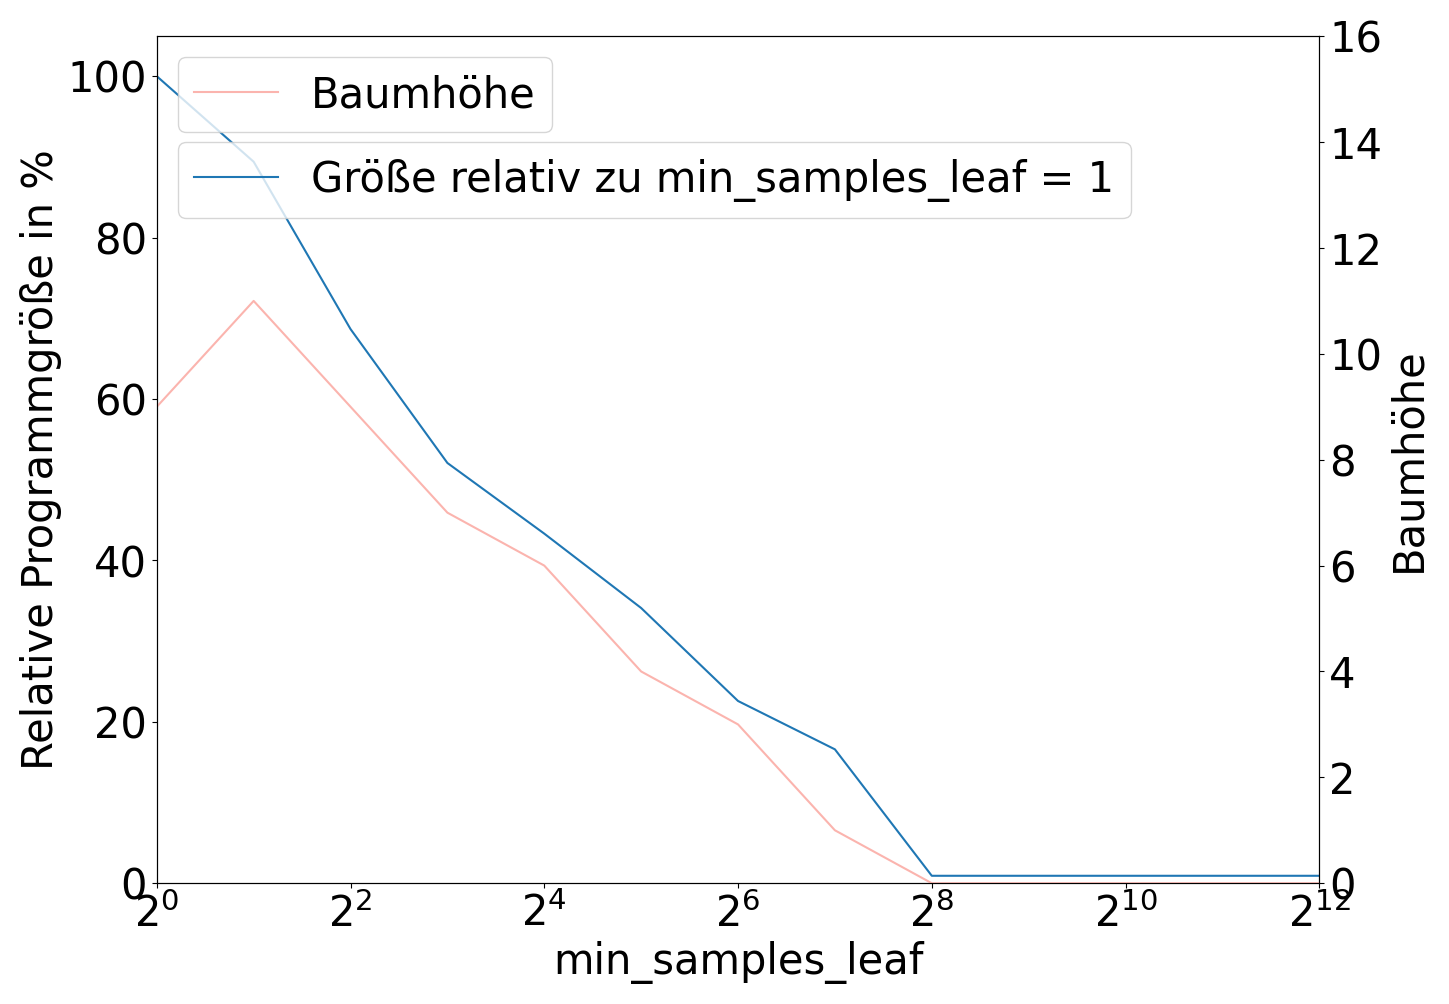
\includegraphics[width=0.48\linewidth]{images/min_samples_leaf_small.png}}\hfill%
\subfigure[Trainingsmengengröße: 7629]{\label{subfig:msl_big}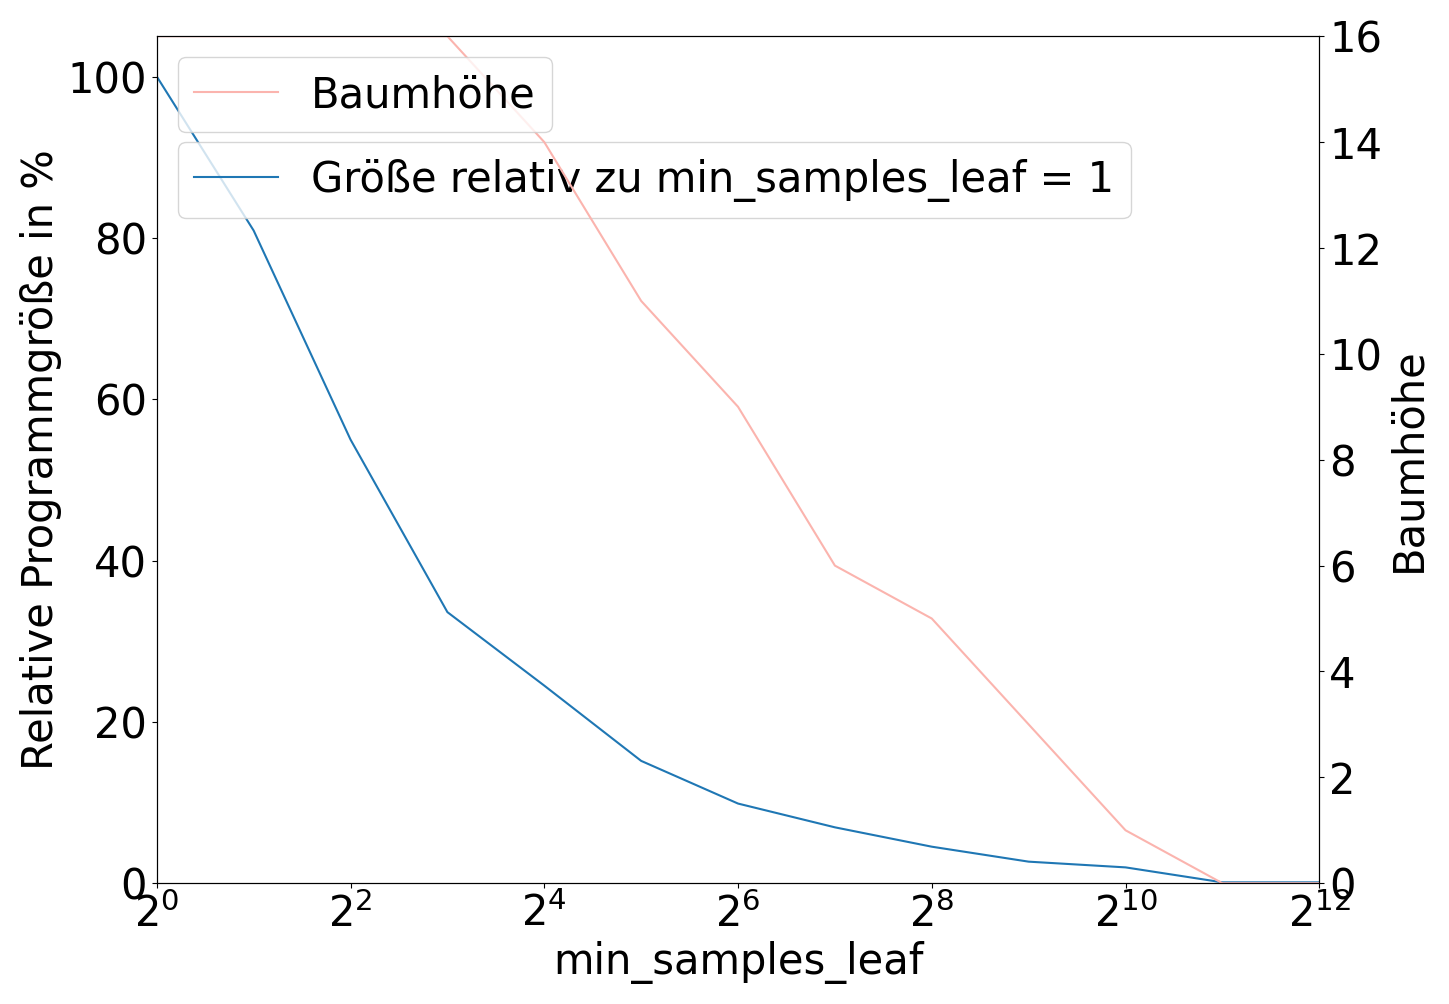
\includegraphics[width=0.48\linewidth]{images/min_samples_leaf_big.png}}%
}{Auswirkung der minimalen Blattgröße auf Programmgröße und Baumhöhe.}{fig:msl}
\newline
\newline
Es kann nicht argumentiert werden, dass ein Wert für die Blattgröße besser ist als ein Anderer, da die Klassifizierungsgenauigkeit auf der Trainingsmenge keine Aussage über die Klassifizierungsgenauigkeit auf
der Testmenge treffen kann. Eine hohe Klassifizierungsgenauigkeit auf Trainingsmenge muss nicht umbedingt eine hohe Klassifizierungsgenauigkeit auf der Testmenge implizieren. Allerdings können so vermeintlich
höhere Entscheidungsbäume ausgewählt werden, da diese weniger Programmspeicher benötigen im Vergleich zu gleich hohen Entscheidungsbäumen mit einer geringeren Blattgröße. Dieser Parameter vergrößert folglich
den Suchraum. Bei kleinen Trainingsmengen ist eine Blattgröße über 1 nur sinnvoll, wenn der größte Entscheidungsbaum, der generiert werden kann, nicht innerhalb der Restriktionen des Programmspeichers liegt.
\subsection{Minimierung der Instruktionen eines Vergleichs}
Ein Vergleich in einem Entscheidungsbaum wurde in Kapitel \ref{sec:cCodeTree} als Abzweigungsexpression mit einem Test definiert. Der Compiler erzeugt für den gleichen Programmcode verschieden viele Instruktionen
je nach Wahl des Datentyps.
\newline
\newline
Listing \ref{lst:assemblyVergleich} zeigt die Komplexität eines einzigen Vergleichs in Instruktionen eines Gleitkommazahlvergleichs. Zeile 1 bis 4 lädt die konstante Gleitkommazahl in 4 hintereinander liegende
8-Bit Register. Zeile 5 bis 7 lädt den Zeiger, der auf die Feature-Menge zeigt, und inkrementiert ihn um 36, um auf das 9. Feature zuzugreifen. In Zeile 8 bis 11 wird das Feature in die Register geladen. Zeile 12 bis 15 führen die
Vergleichsfunktion aus. Damit benötigt ein Vergleich insgesamt 15 Instruktionen.
\begin{lstlisting}[label=lst:assemblyVergleich,caption={Vergleich von Feature als Gleitkommazahl mit konstanter Gleitkommazahl.}]
01: ldi r18,lo8(33)
02: ldi r19,lo8(-92)
03: ldi r20,lo8(69)
04: ldi r21,lo8(60)
05: ldd r26,Y+5
06: ldd r27,Y+6
07: adiw r26,36
08: ld r22,X+
09: ld r23,X+
10: ld r24,X+
11: ld r25,X
12: sbiw r26,36+3
13: call __lesf2
14: cp __zero_reg__,r24
15: brge .+2
\end{lstlisting}
Zu vermeiden sind Zeile 5 bis 11, indem alle Features nur einmal in Register geladen werden. Dies ist allerdings nur möglich, wenn die Größe der Feature-Menge nicht 32~Byte übersteigt bei dem
ATmega328P. Zusätzlich müssten noch Bytes verfügbar sein, um die Konstanten zu laden. Die Feature-Menge der Schwerpunktverteilung beinhaltet 10 Einträge. Der Ansatz mit Gleitkommazahlen ist mit 40 Bytes zu groß.
Der Ansatz mit Ganzzahlen kann diese Optimierung mit 20~Byte ausnutzen. Der Compiler führt diese Optimierung bereits automatisch durch. Wenn die Feature-Menge zu groß ist, werden aus diesem Grund regelmäßig
Register verdrängt, wodurch zusätzlich Instruktionen entstehen. Die Anzahl der Instruktionen können reduziert werden, indem die Größe der Feature-Menge reduziert wird, sodass die Feature-Menge und eine
zusätzliche Konstante des gleichen Datentyps den Registerspeicher nicht übersteigen.
\newline
\newline
Der Datentyp \texttt{Float} ist sehr teuer für einen 8-Bit Prozessor, da immer 4~Register benötigt werden und gegebenenfalls zusätzliche Funktionen, die die fehlende Hardwareunterstüzung ergänzen.
Idealerweise sollte für die Feature-Menge und die Vergleiche ein 8-Bit Datentyp gewählt werden. Damit werden einerseits weniger Register benötigt, wodurch wiederrum die Feature-Menge größer sein kann,
und andererseits können hardwareunterstützte Vergleichsinstruktionen benutzt werden. Dies verringert die Anzahl der Instruktionen signifikant. Folglich vermindert ein kleinerer Datentyp die Anzahl der
Instruktionen signifikant. Listing \ref{lst:assemblyVergleich8Bit} zeigt einen Vergleich von einem 8-Bit Datentyp. Im Kontrast zum Vergleich mit Gleitkommazahlen, werden 66,6\% weniger Instruktionen
benötigt.
\begin{lstlisting}[label=lst:assemblyVergleich8Bit,caption={Vergleich von 8-Bit Feature mit konstanter 8-Bit Zahl.}]
01: adiw r26,4
02: ld r24,X
03: sbiw r26,4
04: cpi r24,lo8(124)
05: brge .L3
\end{lstlisting}
\subsection{Minimierung der Instruktionen einer Rückgabe}
Die Rückgabe der Klassifizierung in einem Entscheidungsbaum kann auf zwei Arten stattfinden. Einerseits kann lediglich die Klasse mit der höchsten Wahrscheinlichkeit zurückgegeben werden. Andererseits kann die
Wahrscheinlichkeitsverteilung zurückgegeben werden, sodass die nächste Ebene die Entscheidung trifft. In Kapitel \ref{sec:cCodeTree} wurde letzteres vorgestellt, da in der nächsten Ebene der Wahlklassifizierer
die Entscheidungsbäume im Ensemble mit Hilfe ihrer Wahrscheinlichkeitsverteilungen zusammenfasst.
\newline
\newline
Listing \ref{lst:assemblyBlattReturn} zeigt die Instruktionen die für die Zuweisung zu vier Klassen von 1.0, 0.0, 0.0 und 0.0 generiert werden. Für jede Klasse wird die Konstante Wahrscheinlichkeit in Register geladen
und anschließend in den Rückgabeparameter gespeichert. In diesem Fall muss nur für die erste Klasse eine Konstante geladen werden, da jede andere Klasse 0 ist. Das heißt, dass im schlimmsten Fall 33
Instruktionen benötigt werden, anstatt 21. Der Compiler führt hier bereits eine Optimierung aus, indem für jedes Ergebnis ein eigener \textit{Basic block} (Eine Datenstruktur die Instruktionen mit einer Annotation
zusammenfasst)erzeugt wird. Zusätzlich könnte kein C-Code generiert werden für eine Zuweisungen mit 0. Dies erfordert aber, dass der Rückgabeparameter mit 0 vorinitialisiert ist.
\newpage
\begin{lstlisting}[label=lst:assemblyBlattReturn,caption={Beispiel der Instruktionen einer Rückgabe der Wahrscheinlichkeitsverteilung eines Entscheidungsbaumes mit 4~Klassen.}]
01: ldi r24,0
02: ldi r25,0
03: ldi r26,lo8(-128)
04: ldi r27,lo8(63)
05: st Z,r24
06: std Z+1,r25
07: std Z+2,r26
08: std Z+3,r27
09: std Z+4,__zero_reg__
10: std Z+5,__zero_reg__
11: std Z+6,__zero_reg__
12: std Z+7,__zero_reg__
13: std Z+8,__zero_reg__
14: std Z+9,__zero_reg__
15: std Z+10,__zero_reg__
16: std Z+11,__zero_reg__
17: std Z+12,__zero_reg__
18: std Z+13,__zero_reg__
19: std Z+14,__zero_reg__
20: std Z+15,__zero_reg__
21: ret
\end{lstlisting}
Eine weitere Optimierung ist den Wahlklassifizierer diskret zu modellieren. Dabei wird für jede Rückgabe des Entscheidungsbaumes ein einstimmiges Ergebnis angenommen, d. h. es wird die Klasse mit der
höchsten Wahrscheinlichkeit in jedem Baum zurückgegeben und nicht mehr die Wahrscheinlichkeitsverteilung. Dadurch werden lediglich die erkannten Klassen
gezählt, anstatt die Wahrscheinlichkeitsverteilungen zu addieren. Listing \ref{lst:assemblyBlattReturnDiskret} zeigt, dass sich die Anzahl der Instruktionen für eine Rückgabe auf genau 2~Instruktionen
reduzieren. Zusätzlich kann der Compiler diese Rückgabe in Basic blocks extrahieren, wodurch lediglich eine Sprunginstruktion benötigt wird. Diese Optimierung ist bei dem diskreten Wahlklassifizierer noch
effektiver, da es genau $N$ verschiedene Rückgabewerte gibt, für $N$ mögliche Klassen. Im schlimmsten Fall reduzieren sich die Anzahl der Instruktionen pro Rückgabe um $\frac{100}{1 + 4N}$\%
und im besten Fall um $\frac{100}{1 + 8N}$\%.
\begin{lstlisting}[label=lst:assemblyBlattReturnDiskret,caption={Beispiel des Assemblycodes der Rückgabe eines diskreten Wahlklassifizierers.}]
01: ldi r24,lo8(1)
02: ret
\end{lstlisting}
Der Nachteil dieses Ansatzes ist, dass die Ergebnisse instabil werden können, wenn viele Rückgaben nur über eine knappe Mehrheit verfügen. Das ist insbesondere der Fall in Kombination mit einem hohen Wert
für die Blattgröße, da dieser die Anzahl der Blattknoten mit Einträgen aus verschiedenen Klassen potenziell erhöht. Diese Optimierung kann auf eine gefundene Lösung angewendet werden, die zu groß für den
Programmspeicher ist. Anschließend sollte die Klassifizierungsgenauigkeit revalidiert werden. Tests haben ergeben, dass die Klassifizierungsgenauigkeit geringfügig schwankt. Folglich kann sich die
Klassifizierungsgenauigkeit auf der Testmenge auch erhöhen.
\newline
\newline
Denkbar wäre ein hybrider Ansatz, der bei einem eindeutigen Ergebnis die Klasse zurück gibt und ansonsten die Wahrscheinlichkeitsverteilung. Die \glqq Eindeutigkeit\grqq\ kann über
einen Schwellenwert $\delta$ definiert sein. Ein Schwellenwert von $\delta=0$ würde an der Korrektheit nichts ändern, würde aber im schlimmsten Fall die Programmgröße nicht verringern.
Tests haben ergeben, dass es immer eindeutige Ergebnisse gibt, weswegen diese Optimierung immer angewendet werden sollte.

\chapter{Evaluation}
Kleine eingebettete Systeme weisen eine stark limitierte Hardware auf. Dafür sind sie aber sehr klein und verbrauchen wenig Energie. Verschiedene Konfigurationen wurden in dieser Arbeit untersucht. Die gefundene
Lösung muss nicht nur eine hohe Klassifizierungsgenauigkeit erzielen, sondern auch auf lauffähig sein auf einem kleinen eingebetteten System, d. h. nicht mehr als den verfügbaren RAM und Programmspeicher nutzen und in
einer passablen Zeit terminieren.
\newline
\newline
Dieses Kapitel untersucht zuerst die Erkennungsgenauigkeit der besten Konfigurationen, die gefunden wurden, je Featuremenge. Die beste Konfiguration wird anschließend auf die Ausführungszeit
und Ressourcenverbrauch auf dem ATmega328P hin analysiert. Dabei wird auf mögliche Optimierungen eingegangen, um die Ausführungszeit und den Ressourcenverbrauch zu senken.

\section{Klassifizierungsgenauigkeit}
Es werden drei Features näher betrachtet. Motion History, Helligkeitsverteilung und Schwerpunktverteilung. Daraus wurden vier Feature-Mengen generiert, die zum Trainieren genutzt werden. Insgesamt wurden 22528
verschiedene Konfigurationen trainiert und getestet, die in Kapitel \ref{sec:Training} beschrieben wurden. Jede Konfiguration nutzt zum Trainieren eine Kombination aus der Trainingsmenge von Feng und Kubik,
sowie die Gestentestmenge und die Nullgestenmenge, die in Kapitel \ref{sec:DymelData} beschrieben wurden. Die Trainingsmenge beinhaltet insgesamt 7629 Handgesten. Davon wird 50\% zum Trainieren und 50\% zum
Validieren und Optimieren auf Basis der Monte Carlo Methode benutzt.
\newline
\newline
Unter jeder Feature-Menge werden jeweils drei Kategorien analysiert. Die erste Kategorie zeigt die beste Konfiguration, die ohne Restriktion des Programmspeichers gefunden wurde. Die zweite Kategorie hat eine Restriktion
von 48 kB und die dritte Kategorie hat eine Restriktion von 32 kB. Diese beziehen sich auf den Programmspeicher des ATmega4809 und ATmega328P, die im Rahmen der Fallstudie verwendet werden \cite{venzkeArticle}.
Dabei werden immer 4 kB abgezogen, da diese für andere systemrelevante Funktionen reserviert sind. Die beste Konfiguration einer Kategorie maximiert die Summe
der Klassifizierungsgenauigkeiten der Testmenge von Klisch, der Gestentestmenge und der Nullgestentestmenge. Dabei wird stets die optimierte Programmgröße der Konfiguration betrachtet, nachdem alle Optimierungen aus Kapitel
\ref{sec:eval_size} angewendet wurden.
\newline
\newline
In der Analyse werden die verschiedenen Feature-Mengen im Hinblick auf die Klassifizierungsgenauigkeit der Testmenge von Klisch, der Gestentestmenge, der Nullgestentestmenge und den synthetischen
Helligkeitstestmengen untereinander verglichen und mit den Ergebnissen von Giese verglichen. Es wird ausschließlich mit Giese verglichen, da seine Ergebnisse die beste Klassifizierungsgenauigkeit,
geringste Ausführungszeit und geringsten Ressourcenverbrauch erzielte. Außerdem wird die Auswirkung von verschiedenen Waldgrößen auf die Klassifizierungsgenauigkeit untersucht. Anzumerken ist, dass
lediglich die Testmenge von Klisch vergleichbar mit den Ergebnissen von Giese ist, da die Gestentestmenge, Nullgestentestmenge und Helligkeitstestmengen erst im Laufe dieser Arbeit entstanden sind.

\subsection{Helligkeitsverteilung}
\begin{table}[h!]
    \centering
    \begin{tabular}{ | l | c | c | c |}
        \hline
        Konfiguration & Beste & Unter 44 kB & Unter 28 kB \\\hline
        Ensemble-Methode & ExtraTrees & ExtraTrees & ExtraTrees \\\hline
        Maximalhöhe & 14 & 10 & 15 \\\hline
        Waldgröße & 10 & 6 & 1 \\\hline
        Blattgröße (min\_samples\_leaf) & 4 & 4 & 4 \\\hline
        Programmgröße in Bytes & 76628 & 33284 & 9364 \\\hline
        Genauigkeit Testmenge von Klisch & 74,0\% & 63,5\% & 67,7\% \\\hline
        Genauigkeit Gestentestmenge & 74,1\% & 79,2\% & 76,6\% \\\hline
        Genauigkeit Nullgestentestmenge & 69,0\% & 71,0\% & 67,0\% \\\hline
    \end{tabular}
    \caption{Die beste Konfigurationen der Helligkeitsverteilung.}
    \label{tab:helligkeitsverteilung}
\end{table}
\begin{figure}[h!]
    \centering
    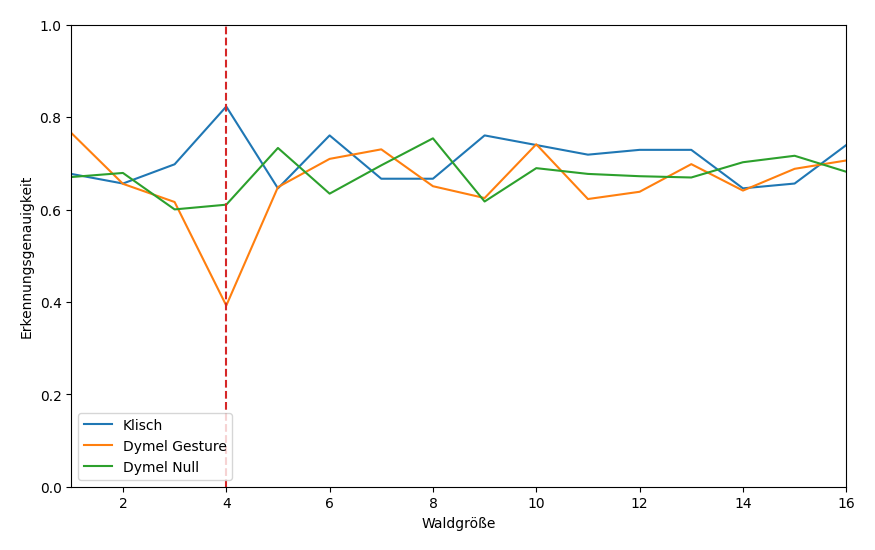
\includegraphics[width=\linewidth]{images/helligkeitsverteilung_acc_per_size.png}
    \caption{Die besten Konfigurationen pro Waldgröße mit der Helligkeitsverteilung.}
    \label{fig:helligkeitsverteilung_per_forest_size}
\end{figure}
Die Featuremenge der Helligkeitsverteilung beinhaltet insgesamt 12 Features. Jeweils 6 Feature repräsentieren Zeitfenster der minimalen Helligkeit und der maximalen Helligkeit. Die Zeitfenster wurden
geometrisch zusammengefasst.
\newline
\newline
Aus der Tabelle \ref{tab:helligkeitsverteilung} sind die besten Konfigurationen jeder Kategorie zu entnehmen. Die beste Konfiguration wurde mit der Ensemble-Methode \textit{ExtraTrees} gefunden.
Sie erzielt eine Klassifizierungsgenauigkeit von 74\% auf der Testmenge von Klisch und ist damit 25,2\% schlechter als das neuronale Netzwerk von Giese \cite{gieseThesis}. Außerdem wird 74\% der Gestentestmenge
und 69\% der Nullgestentestmenge korrekt klassifiziert.
\newline
\newline
Wird die Kategorie \textit{Beste} und die Kategorie \textit{Unter 28 kB} vergleichen, nimmt die Gesamtklassifizierungsgenauigkeit nur um 1,94\% ab. Dabei reduziert sich die Programmgröße um 87,8\%.
Ein ähnliches Verhalten ist auch in Abbildung \ref{fig:helligkeitsverteilung_per_forest_size} zu erkennen. Dort ist nur ein geringer Zuwachs der Gesamtklassifizierungsgenauigkeit mit der zunehmenden
Waldgröße zu beobachten.
\subsection{Motion History}
\begin{table}[h!]
    \centering
    \begin{tabular}{ | l | c | c | c |}
        \hline
        Konfiguration & Beste & Unter 44 kB & Unter 28 kB \\\hline
        Ensemble-Methode & ExtraTrees & ExtraTrees & ExtraTrees \\\hline
        Maximalhöhe & 10 & 11 & 9 \\\hline
        Waldgröße & 16 & 7 & 6 \\\hline
        Blattgröße (min\_samples\_leaf) & 1 & 2 & 1 \\\hline
        Programmgröße in Bytes & 84200 & 40456 & 22804 \\\hline
        Genauigkeit Testmenge von Klisch & 68,8\% & 67,7\% & 62,5\% \\\hline
        Genauigkeit Gestentestmenge & 74,5\% & 67,6\% & 68,5\% \\\hline
        Genauigkeit Nullgestentestmenge & 68,3\% & 64,4\% & 67,6\% \\\hline
    \end{tabular}
    \caption{Die besten Konfigurationen der Feature-Menge Motion History.}
    \label{tab:motion_history}
\end{table}
\begin{figure}[h!]
    \centering
    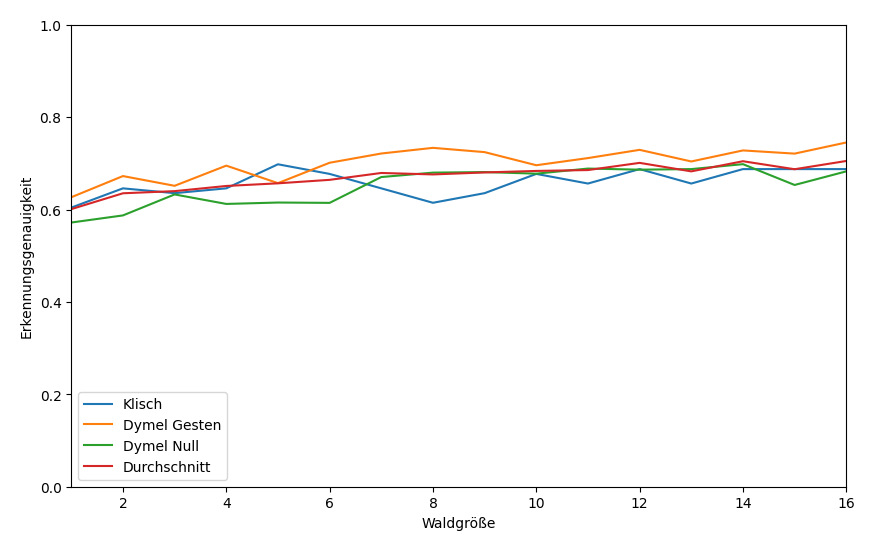
\includegraphics[width=\linewidth]{images/motion_history_acc_per_size.png}
    \caption{Die besten Modelle pro Waldgröße der Feature-Menge Motion History.}
    \label{fig:motion_history_per_forest_size}
\end{figure}
Die Feature-Menge Motion History beinhaltet für jeden Pixel ein Feature, das der Definition des Motion History Image folgt (Formel \ref{formular:mhi}), wobei $\tau=100$ und $\delta=\frac{\tau}{\#Bilder}$ ist.
\newline
\newline
Aus Tabelle \ref{tab:helligkeitsverteilung} sind die besten Konfigurationen jeder Kategorie zu entnehmen. Die beste Konfiguration wurde wieder mit der Ensemble-Methode \textit{ExtraTrees} gefunden.
Das Modell erzielt eine Klassifizierungsgenauigkeit von 68,8\% auf der Testmenge von Klisch, 74\% auf der Gestentestmenge und 69\% auf der Nullgestentestmenge. Im Vergleich zu der Helligkeitsverteilung
wird mehr Programmspeicher benötigt und die Gesamtklassifizierungsgenauigkeit ist 1,84\% schlechter.
\newline
\newline
Wird die Kategorie \textit{Beste} mit der Kategorie \textit{Unter 28~kB} verglichen, nimmt die Gesamtklassifizierungsgenauigkeit nur um 4,3\% ab. Dabei reduziert sich die Programmgröße um 72,9\%.
Abbildung \ref{fig:motion_history_per_forest_size} zeigt, dass die Klassifizierungsgenauigkeit im Durchschnitt sich mit zunehmender Waldgröße erhöht. Im Vergleich zur Helligkeitsverteilung, ist der Zuwachs größer.
Wenn der Suchraum nicht auf eine Waldgröße von 16~Bäumen begrenzt wäre, würde die beste Konfiguration vermutlich besser sein. Allerdings würde sich auch die Programmgröße signifikant erhöhen.
\newline
\newline
Die Motion History kann mit ausschließlich 8-Bit Integer implementiert werden und hat damit die geringste WCET und Programmgröße pro Baum, weswegen die beste Konfiguration mit einer Waldgröße von 16~Bäumen nicht deutlich
größer ist, als die der Helligkeitsverteilung mit einer Waldgröße von 10~Bäumen.

\subsection{Schwerpunktverteilung mit Gleitkommazahlen}
\begin{table}[h!]
    \hspace{-0.5cm}
    \begin{tabular}{ | l | c | c | c | c |}
        \hline
        Konfiguration & Beste & Unter 60 kB & Unter 28 kB & Unter 14 kB \\\hline
        Ensemble-Methode & Boosting & Boosting & RandomForest & Bagging  \\\hline
        Maximalhöhe & 20 & 19 & 10 & 7 \\\hline
        Waldgröße & 10 & 6 & 4 & 3 \\\hline
        min\_samples\_leaf & 8 & 8 & 2 & 8 \\\hline
        Programmgröße in Bytes & 83304 & 43678 & 20188 & 6656 \\\hline
        Genauigkeit Testmenge von Klisch & 94,8\% & 94.8\% & 89,6\% & 87,5\% \\\hline
        Genauigkeit Gestentestmenge & 97,0\% & 96,1\% & 95,6\% & 94,1\% \\\hline
        Genauigkeit Nullgestentestmenge & 92,2\% & 91,1\% & 88,8\% & 89,9\% \\\hline
    \end{tabular}
    \caption{Beste Konfigurationen der Schwerpunktverteilung mit Gleitkommazahlen.}
    \label{tab:schwerpunktverteilung_float}
\end{table}
\begin{figure}[h!]
    \centering
    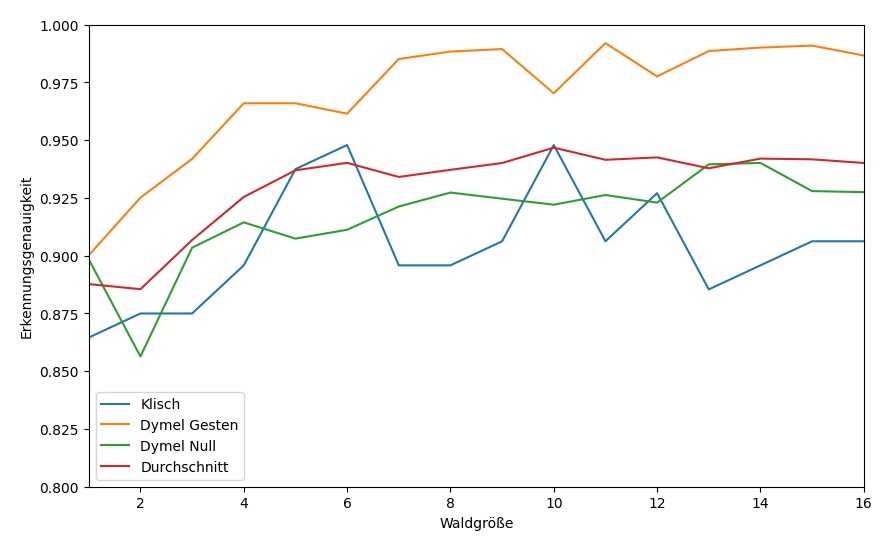
\includegraphics[width=\linewidth]{images/cocd_float_acc_per_size.png}
    \caption{Die beste summierte Erkennungsgenauigkeit pro Waldgröße der Schwerpunktverteilung mit Gleitkommazahlen.}
    \label{fig:cocd_float_per_forest_size}
\end{figure}
Die Featuremenge Schwerpunktverteilung mit Gleitkommazahlen folgt der Definition aus Sektion \ref{sec:schwerpunktverteilung} und beinhaltet insgesamt 10 Einträge, wobei jeweils 2 Einträge die X und Y
Koordinate des Schwerpunktes darstellen in insgesamt 5 Zeitfenstern.
\newline
\newline
Die beste Konfiguration wurde mit der Ensemble-Methode Boosting erzielt (siehe Tabelle \ref{tab:schwerpunktverteilung_float}). Mit einer Erkennungsgenauigkeit von 94,8\% auf der Testmenge von Klisch
ist dieser Ansatz nur 5,2\% schlechter als das neuronale Netz von Giese \cite{gieseThesis}. Es ist anzumerken, dass mit einer kleineren Trainingsmenge ohne die Gestentrainingsmenge und Nullgestentrainingsmenge eine Lösung
gefunden wurde, die 97,9\% erzielte und damit nur 2,1\% schlechter ist. Außerdem werden 97\% der Gestentestmenge und 92,2\% der Nullgestentestmenge korrekt klassifiziert.
\newline
\newline
Im Vergleich zu der Helligkeitsverteilung und Motion History ist die Erkennungsgenauigkeit dieses Ansatzes signifikant besser, sogar wenn nur 6656 Byte Programmspeicher verwendet werden. Wird die beste Konfiguration mit
der \textit{Unter 14 kB} verglichen, nimmt die Gesamterkennungsganuigkeit nur um 4,17\% ab bei der Reduktion der Programmgröße von 92\%. Dies verspricht, dass mit zunehmender Waldgröße der die Erkennungsgenauigkeit steigt.
Abbildung \ref{fig:cocd_float_per_forest_size} zeigt, dass dies zwar der Fall ist, aber schon ab einer Waldgröße von 6 ist die Durchschnittliche Erkennungsgenauigkeit keinen signifikanten Zuwachs mehr verzeichnet.
Dementsprechend ist der Unterschied der Gesamterkennungsgenauigkeit der besten Konfiguraiton und \textit{Unter 60 kB} mit 0,7\% nicht groß, wodurch sich dieses Feature gut für kleine eingebettete Systeme mit
wenig Programmspeicher eignet.
\subsection{Schwerpunktverteilung mit Ganzzahlen}
\begin{table}[h!]
    \hspace{-0.5cm}
    \begin{tabular}{ | l | c | c | c |}
        \hline
        Konfiguration & Beste & Unter 44 kB \& 28 kB & Unter 14 kB \\\hline
        Ensemble-Methode & ExtraTrees & Random Forest & Random Forest \\\hline
        Maximalhöhe & 21 & 13 & 12 \\\hline
        Waldgröße & 11 & 7 & 3 \\\hline
        Blattgröße (min\_samples\_leaf) & 2 & 4 & 1 \\\hline
        Programmgröße in Bytes & 76200 & 21532 & 11012 \\\hline
        Genauigkeit Testmenge von Klisch & 95,8\% & 91,7\% & 86,5\% \\\hline
        Genauigkeit Gestentestmenge & 98,8\% & 97,1\% & 95,5\% \\\hline
        Genauigkeit Nullgestentestmenge & 95,6\% & 94,5\% & 88,9\% \\\hline
    \end{tabular}
    \caption{Die besten Konfigurationen der Schwerpunktverteilung mit Ganzzahlen.}
    \label{tab:schwerpunktverteilung_int}
\end{table}
\begin{figure}[h!]
    \centering
    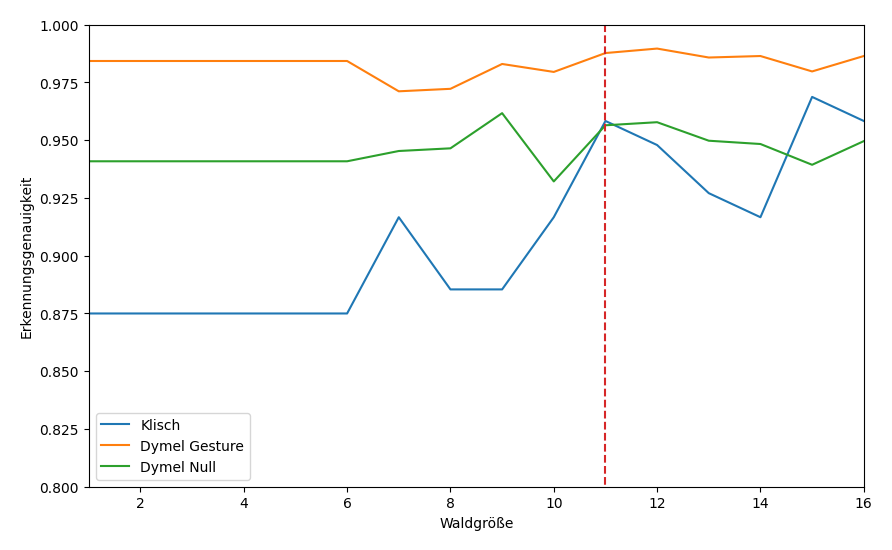
\includegraphics[width=\linewidth]{images/cocd_int_acc_per_size.png}
    \caption{Die besten Konfigurationen pro Waldgröße der Schwerpunktverteilung mit Ganzzahlen.}
    \label{fig:cocd_int_per_forest_size}
\end{figure}
Die Featuremenge Schwerpunktverteilung mit Ganzzahlen folgt der Definition aus Kapitel \ref{sec:schwerpunktverteilung} und beinhaltet insgesamt 10 Einträge. Jeweils 2 Einträge bilden die X und Y
Koordinate des Schwerpunktes. Damit spiegeln 10 Einträge insgesamt 5 Zeitfenster wieder.
\newline
\newline
Aus der Tabelle \ref{tab:schwerpunktverteilung_int} sind die besten Konfigurationen jeder Kategorie zu entnehmen. Die beste Konfiguration wurde mit der Ensemble-Methode ExtraTrees gefunden.
Mit einer Klassifizierungsgenauigkeit von 95,8\% auf der Testmenge von Klisch ist dieser Ansatz nur 3,2\% schlechter als das neuronale Netz von Giese \cite{gieseThesis}. Es wurde aber auch eine Konfiguration
gefunden, die 96,9\% der Testmenge von Klisch korrekt klassifiziert und damit nur 2,1\% schlechter ist. Diese maximiert aber in keiner Kategorie die Gesamtklassifizierungsgenauigkeit.
Außerdem werden 98,8\% der Gestentestmenge und 95,6\% der Nullgestentestmenge korrekt klassifiziert. Es wurde kein Entscheidungswald gefunden, der weniger als 44 kB Programmspeicher benötigt und besser ist als die
Konfiguration in der Kategorie \textit{Unter 28 kB}.
\newline
\newline
Der Ansatz mit Ganzzahlen erzielte eine 2,1\% höhere Gesamtklassifizierungsgenauigkeit als der Ansatz mit Gleitkommazahlen. Der 16-Bit Integer Datentyp erlaubt der Schwerpunktverteilung mit Ganzzahlen unter jeder
Restriktion größere Entscheidungswälder zu bilden, als die Schwerpunktverteilung mit Gleitkommazahlen. Abbildung \ref{fig:cocd_int_per_forest_size} zeigt einen Zuwachs der durchschnittlichen Klassifizierungsgenauigkeit
mit zunehmender Waldgröße. Es ist auszugehen, dass eine noch bessere Konfiguration gefunden werden könnte, wenn der Suchraum auf eine größere Waldgröße erweitert wird. Ähnlich wie die Schwerpunktverteilung mit
Gleitkommazahlen ist der Zuwachs der durchschnittlichen Klassifizierungsgenauigkeit ab einer Waldgröße von 7 Bäumen gering. Somit kann bereits bei einer geringen Programmgröße eine hohe Klassifizierungsgenauigkeit
erzielt werden. Damit eignet sich die Schwerpunktverteilung mit Ganzzahlen ebenfalls für kleine eingebettete Systeme.

\subsection{Kombinierte Schwerpunktverteilung}
\begin{table}[h!]
    \centering
    \begin{tabular}{ | l | c | c | c | c |}
        \hline
        Konfiguration & Beste & Unter 44 kB & Unter 28 kB \\\hline
        Schwerpunktverteilung Gleitkommazahl & Beste & Unter 14 kB & Unter 14 kB \\\hline
        Schwerpunktverteilung Ganzzahlen & Beste &  Unter 28 kB & Unter 14 kB \\\hline
        Programmgröße in Bytes & - & 33276 & 20252 \\\hline
        Genauigkeit Testmenge von Klisch & 94,8\% & 87,5\% & 87,5\% \\\hline
        Genauigkeit Gestentestmenge & 99,0\% & 97,7\% & 96,9\% \\\hline
        Genauigkeit Nullgestentestmenge & 95,8\% & 92,9\% & 92,5\% \\\hline
    \end{tabular}
    \caption{Die besten Konfigurationen der kombinierten Schwerpunktverteilung.}
    \label{tab:schwerpunktverteilung_int_and_float}
\end{table}
Die kombinierte Schwerpunktverteilung vereint die Schwerpunktverteilung mit Ganzzahlen und Gleitkommazahlen. Das erscheint sinnvoll, da der Ansatz mit Ganzzahlen invariant zu einem Offset in der
Helligkeit ist und der Ansatz mit Gleitkommazahlen invariant zur Skalierung der Helligkeit.
\newline
\newline
Es wird davon ausgegangen, dass der jeweilige Klassifizierer entweder ein Ergebnis mit einer deutlichen Mehrheit zurückgibt oder ein Ergebnis mit einer knappen Mehrheit. Für jedes Lichtverhältniss, hat mindestens ein
Klassifizierer eine deutliche Mehrheit. Damit erzielt die Kombination eine Mehrheit bei der korrekten Klasse. Die besten Konfigurationen der beiden Ansätze werden mit einem Wahlklassifizierer vereint.
Das heißt, die Wahrscheinlichkeitsverteilungen der Wahlklassifizierer der jeweiligen Ansätze werden zu gleichen Anteilen addiert.
\newline
\newline
Die Kombination der besten Konfigurationen beider Ansätze erzielt eine Klassifizierungsgenauigkeit von 94,8\% auf der Testmenge von Klisch. Dies entspricht der Klassifizierungsgenauigkeit der Schwerpunktverteilung mit
Gleitkommazahlen. 99\% der Gestentestmenge wird korrekt klassifiziert. Das ist besser als beide Ansätze. Die Nullgestestmenge wurde zu 95,8\% korrekt klassifiziert. Dies entspricht der Klassifizierungsgenauigkeit der
Schwerpunktverteilung mit Ganzzahlen. Bei der Kategorie \textit{Unter 44 kB} und \textit{Unter 28 kB} wurde der kombinierte Klassifizierer nie schlechter als der schlechteste Ansatz auf dem die kombinierte
Schwerpunktverteilung basiert.
\newline
\newline
Der Nachteil dieses Ansatzes ist, dass sowohl die Feature-Menge mit Gleitkommazahlen, als auch für Ganzzahlen benötigt wird. Zum einen müssen immer beide Features berechnet werden und zum anderen kann jeder Klassifizierer
nur halb so viel Speicher nutzen. Dadurch ist die Klassifizierungsgenauigkeit jedes Klassifizierers potenziell geringer, als wenn es den vollständigen Speicher zur Verfügung hätte. Bei der Schwerpunktverteilungen ist aber
bereits ab einer geringen Waldgröße kein signifikanter Zuwachs der Klassifizierungsgenauigkeit zu verzeichnen. Deswegen eignet sich die Schwerpunktverteilung besonders gut. Der Vorteil ist, dass der kombinierte
Klassifizierer potenziell robuster ist gegenüber unterschiedliche Lichtverhältnisse.


\subsection{Robustheit gegenüber Lichtverhältnisse}
TODO: For each best configuration per featureset add a line in the plot for scaling and offset invariance.


\section{Ausführungszeit}
\label{sec:eval_speed}
Die Ausführungszeit der Feature-Extrahierung und Klassifizierung ist ausschlaggebend für die mögliche FPS. Diese ermöglicht die Wahrnehmung von schnellen Handgesten. Ist die FPS bereits ausreichend
können leistungschwächere Module verwendet werden, wodurch die Batterielaufzeit verlängert wird oder die Kosten reduziert werden.
\newline
\newline
In dieser Arbeit wird das Arduino Board ATmega328P genutzt. Dieses Board verfügt über eine 8-Bit APU, 2 kB RAM, 32 kB Flash-Speicher und operiert unter 16 MHz \cite{atmega328p}.
Es verfügt nicht über ein Modul zur Verarbeitung von Gleitkommazahlen. Aus diesem Grund sind Operationen mit Gleitkommazahlen besonders teuer und zu vermeiden.
\newline
\newline
Es wird ausschließlich die \textit{Worst-Case-Execution-Time} (WCET) betrachtet. Ausschlaggebend dafür ist der \textit{Worst-Case-Execution-Path} (WCEP) im Kontrollflussgraph \cite{wcc_intro}. Der WCEP
setzt sich zusammen aus dem Vorgang das aktuelle Bild auszulesen, der Extrahierung der Features und der Ausführung des Klassifizierers.
\newline
\newline
Die Auswertung bezieht sich auf die Instruktionen des Programms, die bei der Übersetzung der Firmware durch den \textit{AVR GCC} mit der Optimierungsstufe \texttt{Os} entstehen. Aus dem Handbuch des
ATmega328P \cite{atmega328p} können für jede Instruktion die maximale Anzahl der Zyklen entnommen werden, die im schlimmsten Fall benötigt werden. Die Gesamtausführungszeit berechnet sich aus der Anzahl der Zyklen
multipliziert mit der Zeit pro Zyklus, d. h. bei 16 MHz bedarf ein Zyklus 0,0625 $\mu s$.

\subsection{Feature-Extrahierung}
Die Feature-Extrahierung implementiert die Berechnung der fünf Zeitfenster für die Schwerpunktverteilung. Einerseits muss aus jedem Bild der Schwerpunkt berechnet werden und andererseits müssen die Schwerpunkte
auf fünf Schwerpunkte zusammengefasst werden, die die fünf Zeitfenster repräsentieren.
\newline
\newline
Jedes Mal wenn ein Bild aufgenommen wird, wird der Schwerpunkt dieses Bildes berechnet und gespeichert. Dies reduziert einerseits die WCET, da im WCEP weniger Schwerpunkte berechnet werden müssen, und andererseits
wird weniger Pufferspeicher benötigt pro Bild. Für Gleitkommazahlen reduziert sich der Verbrauch pro Bild von 18 Byte auf 8 Byte und für Ganzzahlen auf 4 Byte. Der kombinierte Ansatz muss beide Schwerpunkte speichern.
Die jeweiligen Schwerpunktkoordinaten berechnen sich mit der in Kapitel \ref{sec:schwerpunktverteilung} beschriebenen Formel. Dabei muss die Summe der Pixel einmalig pro Bild berechnet werden und jeweils die
berechnete X und Y Koordinate im Puffer für den derzeitige Schwerpunkt gespeichert werden. Listing \ref{lst:cocdAlgoCOCDPerPicture} zeigt, wie dies auf dem ATmega328P implementiert ist. Insgesamt werden bei der
Schwerpunktverteilung mit Gleitkommazahlen 201 Zyklen für die einzelnen Instruktionen benötigt (12,5625 $\mu s$). Zusätzlich wird \textit{\_\_floatsisf} sechs mal aufgerufen, \textit{\_\_lesf2} und \textit{\_\_divsf3}
jeweils zwi mal aufgerufen. Die WCET zur Schwerpunktberechnung eines Bildes beläuft sich damit auf 116,5625 $\mu s$. Davon werden 104 $\mu s$ für Gleitkommaoperationen aufgewendet. Der Ansatz mit Ganzzahlen benötigt
keine Gleitkommaoperationen und 57 Zyklen weniger, da die summe der Pixel nicht berechnet werden muss, d. h. es werden für die WCET nur 8,875 $\mu s$ benötigt. Für den kombinierten Ansatz werden zusätzlich vier
Speicherinstruktionen benötigt, die einen Overhead von 0,25 $\mu s$ erzeugen, d. h. es werden für die WCET 116,8125 $\mu s$ benötigt.
\begin{lstlisting}[label=lst:cocdAlgoCOCDPerPicture,caption={Implementierung um den Schwerpunkt für ein Bild zu berechnen.}]
short helligkeits_summe = 0;
for (char i = 0; i < 9; ++i)
    helligkeits_summe += bild_puffer[i];
schwerpunkt_puffer_x[anzahl_bilder_im_puffer] = (float)(bild_puffer[0] + bild_puffer[3] + bild_puffer[6] - bild_puffer[2] - bild_puffer[5] - bild_puffer[8]) / ((float)helligkeits_summe);
schwerpunkt_puffer_y[anzahl_bilder_im_puffer] = (float)(bild_puffer[0] + bild_puffer[1] + bild_puffer[2] - bild_puffer[6] - bild_puffer[7] - bild_puffer[8]) / ((float)helligkeits_summe);
\end{lstlisting}
Wenn ein Handgestenkandidat detektiert wurde, wird für jedes Zeitfenster der Durchschnitt der darin enthaltenden Schwerpunkte berechnet. Die daraus berechneten Schwerpunkte werden als Schwerpunktverteilung bezeichnet.
Listing \ref{lst:cocdAlgo} zeigt den Algorithmus, um die Schwerpunktverteilung aus den Schwerpunkten im Puffer zu berechnen. Zunächst wird bei der Initialisierungsphase das \texttt{zusammenfass\_muster} berechnet
(Kap \ref{sec:schwerpunktverteilung}). Dafür werden im schlimmsten Fall 123 Zyklen für die einzelnen Instruktionen benötigt (7,6875 $\mu s$) und 20 $\mu s$ für die Ganzzahldividierung \textit{\_\_divmodhi4}. Insgesamt
27,6875 $\mu s$. Dieser Teil wird genau 1 mal für alle Richtungen und Schwerpunktverteilungen durchgeführt. Die innere Schleife wird im schlimmsten Fall für die Gesamtgröße des Schwerpunktpuffers durchlaufen.
Jeder Durchlauf benötigt im schlimmsten Fall 27 Zyklen für die einzelnen Instruktionen (1,6875 $\mu s$) und führt \textit{\_\_addsf3} einmal aus. Der WCET für einen Durchlauf beläuft sich damit auf 13,6875 $\mu s$.
Der Ansatz mit Ganzzahlen benötigt im schlimmsten Fall 17 Zyklen (1,125 $\mu s$). Bei einer Gesamtpuffergröße von 125 wird für den Teil der inneren Schleife für die Schwerpunktverteilung mit Gleitkommazahlen
1710,9375 $\mu s$ benötigt, für die Schwerpunktverteilung mit Ganzzahlen 140,625 $\mu s$ und für den kombinierten Ansatz 1851,5625 $\mu s$. Die äußere Schleife benötigt im schlimmsten Fall 57 Zyklen für die einzelnen
Instruktionen (3,5625 $\mu s$) und ruft im Ansatz mit Gleitkommazahlen fünf mal \textit{\_\_floatsisf} und \textit{\_\_divsf3} auf und im Ansatz mit Ganzzahlen fünf mal \textit{\_\_divmodhi4}. Damit beläuft sich der WCET
bei fünf Durchläufen der äußeren Schleife für den Ansatz mit Gleitkommazahlen auf 217,8125 $\mu s$, für den Ansatz mit Ganzzahlen auf 117,8125 $\mu s$ und für den kombinierten Ansatz 335,625 $\mu s$.
\begin{lstlisting}[label=lst:cocdAlgo,caption={Algorithmus um die Schwerpunktverteilung in horizontaler Richtung zu berechnen.}]
Initialisierung.
for (char i = 0; i < 5; ++i) { // Äußere Schleife
    features[i] = 0;
    for (char j = 0; j < zusammenfass_muster[i]; ++j) // Innere Schleife
        features[i] += *(schwerpunkt_puffer_x++);
    features[i] /= ((float)zusammenfass_muster[i]);
}
\end{lstlisting}
Der Schwerpunkt wird jeweils für die horizontale und vertikale Richtung berechnet. Der kombinierte Ansatz berechnet sowohl den Schwerpunkt für Gleitkommazahlen als auch für Ganzzahlen. Die WCET für die Feature-Extrahierung
der Schwerpunktverteilung mit Gleitkommazahlen beläuft sich auf 4001,75 $\mu s\ \approx\ $ 4 ms. Die WCET der Schwerpunktverteilung mit Ganzzahlen beläuft sich auf 553,4375 $\mu s\ \approx\ $ 0,6 ms. Die WCET der kombinierten
Schwerpunktverteilung beläuft sich auf 4518,875 $\mu s\ \approx\ $ 4,5 ms.

\subsection{Tree Evaluation}
\subsection{Ausführung eines Entscheidungswaldes}
Der WCEP eines Entscheidungswaldes setzt sich aus dem WCEP des Wahlklassifizierungsalgorithmus und dem WCEP jedes Entscheidungsbaumes zusammen, der im Wald enthalten ist.
\newline
\newline
Der in Listing \ref{lst:sklearnCCodeTreeVoting} gezeigte Code implementiert den Wahlvorgang. Die Komplexität ist abhängig von der Anzahl der Features $N$ und der Anzahl der Entscheidungsbäume $K$. In
dieser Analyse wird für die Anzahl der Features $N=5$ angenommen.
Jede Stimme eines Entscheidungsbaumes bedarf 18~Zyklen (1,125~$\mu s$), um die Funktion, die den Entscheidungsbaum ausführt, aufzurufen und das Ergebnis des ausgeführten Entscheidungsbaumes auf die Gesamtsumme zu addieren.
Die restlichen Instruktionen bedürfen 64 Zyklen (4~$\mu s$).
\newline
\newline
Die WCET eines Entscheidungswaldes beläuft sich damit auf 4~$\mu s$ + \#Entscheidungsbäume $\cdot$ (1,125~$\mu s$ + WCET der Entscheidungsbäume).
\section{Programmgröße}
\label{sec:eval_size}
Generell gilt, je größer und dichter der Entscheidungswald ist, desto höher ist die Erkennungsgenauigkeit. Aus diesem Grund sollte immer der vollständige Programmspeicher ausgenutzt werden. Allerdings nimmt der
Zuwachs an Erkennungsgenauigkeit mit jeder weiteren Teilung ab bei der Konstruktion eines Entscheidungsbaumes.
\newline
\newline
Scikit-Learn bietet viele Parameter, um die Teilung zu steuern. Dies mag die potentielle
Erkennungsgenauigkeit eines Baumes leicht verringern, kann dafür aber die Größe stark verringern. Dadurch jönnen tiefere Bäume verwendet werden oder mehr Bäume in einem Entscheidungswald, was potentiell
einen größeren Zuwachs der Erkennungsgenauigkeit verspricht.
\newline
\newline
Die Größe und Dichte eines Entscheidungswaldes haben einen direkten Einfluss auf die generierten Instruktionen. Je größer und dichter, desto mehr Instruktionen. Aus diesem Grund soll einerseits der
Zuwachs der Erkennungsgenauigkeit pro Vergleich maximiert werden und andererseits die Instruktionskosten pro Vergleich und Blattkosten minimiert werden.

\subsection{Maximierung des Zuwachses der Klassifizierungsgenauigkeit}
Scikit-Learn bietet viele Parameter an, um den Teilungsprozess bei der Konstruktion zu steuern. Einer dieser Parameter ist \texttt{min\_samples\_leaf}, d. h. die minimale Anzahl an Einträgen der Trainingsmenge
in einem Blatt. Dieser steuert die minimale Anzahl an Einträgen die in einem Kindknoten enthalten sein müssen, nachdem ein Knoten geteilt wurde. Standardmäßig ist der Wert 1. Dadurch entsteht ein sehr fein granularer
Entscheidungsbaum, der viele Blätter mit nur einem Eintrag hat. Das heißt, es wurden Teilungen durchgeführt, die nur zwei Einträge unterteilt haben. Der Zuwachs der Klassifizierungsgenauigkeit ist durch diese
Teilungen sehr gering. Eine Erhöhung in der Blattgröße verspricht, dass Entscheidungsbäume gefunden werden können, die zwar tiefer sind, aber dafür eine bessere Klassifizierungsgenauigkeit pro Vergleich erzielen.
Der Baum kann tiefer werden, da die Grenze des Programmspeichers noch nicht erreicht wurde.
\newline
\newline
Abbildung \ref{fig:msl} zeigt, wie sich der Parameter auf verschieden große Trainingsmengen auswirkt. Betrachtet wird eine Maximalhöhe von 16. Besonders bei großen Trainingsmengen (Abbildung \ref{subfig:msl_big})
kann die Programmgröße mit einer Blattgröße von 8 signifkant sinken, ohne die maximale Baumhöhe zu beeinflussen. Bei kleinen Trainingsmengen (Abbildung \ref{subfig:msl_small}) reduziert bereits bei kleinen Blattgrößen
sich die Programmgröße ebenfalls signifikant. Allerdings wird die maximale Baumhöhe beeinflusst. Besonders bei großen Trainingsmengen wirkt sich der Parameter stärker auf die Programmgröße aus.
Vermutlich, da die Anzahl der Blätter sich signifikant erhöht, je tiefer der Baum ist.
\subfigbox{
\subfigure[Trainingsmengengröße: 1023]{\label{subfig:msl_small}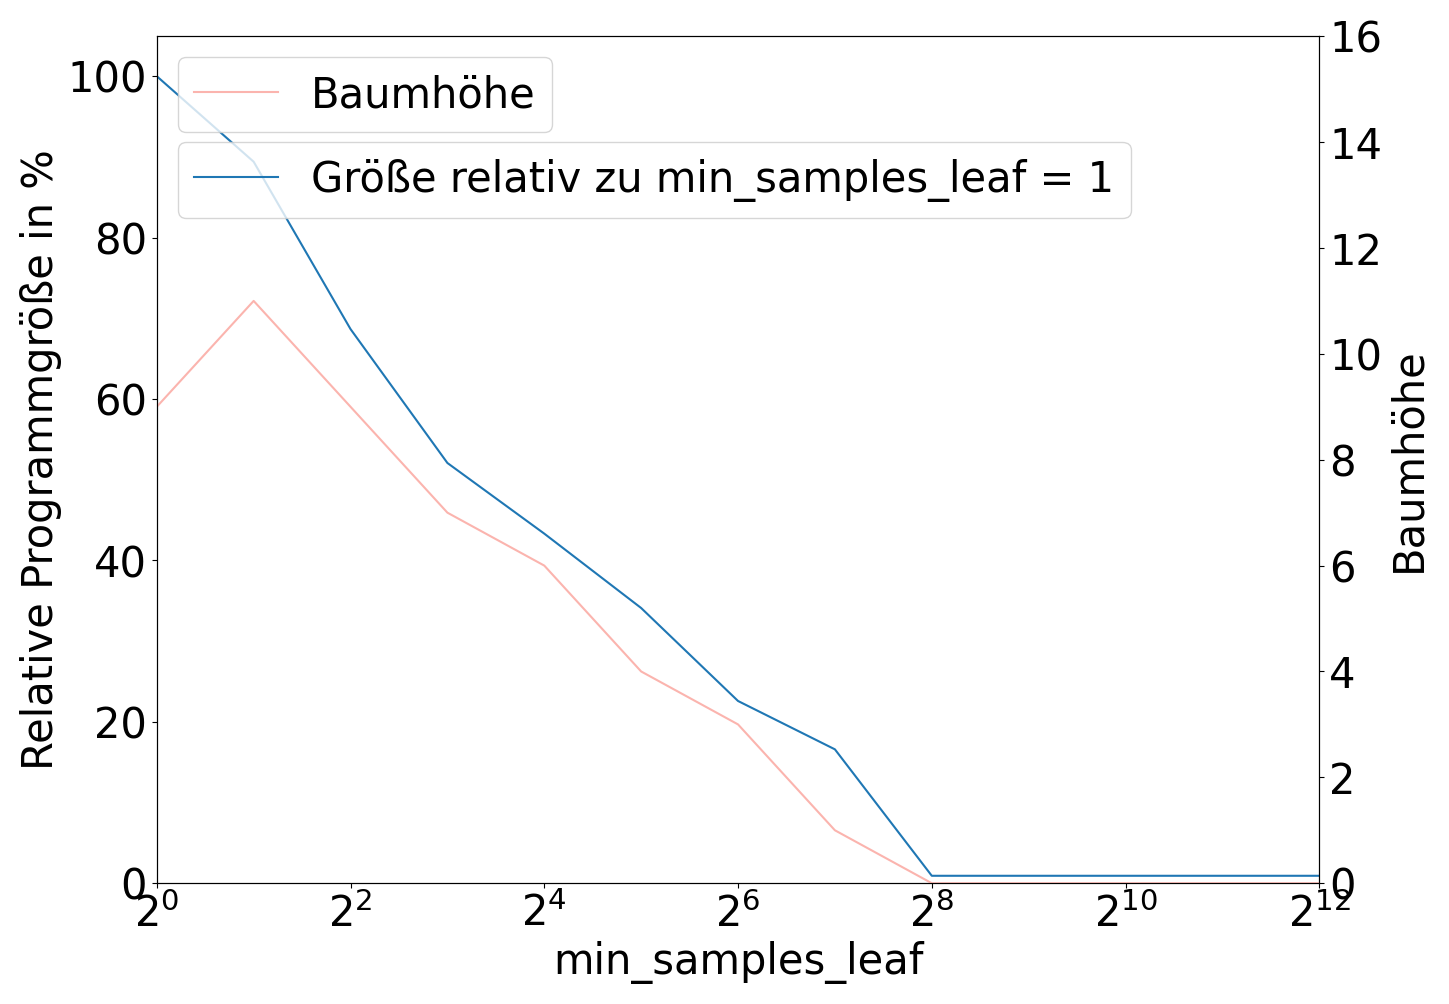
\includegraphics[width=0.48\linewidth]{images/min_samples_leaf_small.png}}\hfill%
\subfigure[Trainingsmengengröße: 7629]{\label{subfig:msl_big}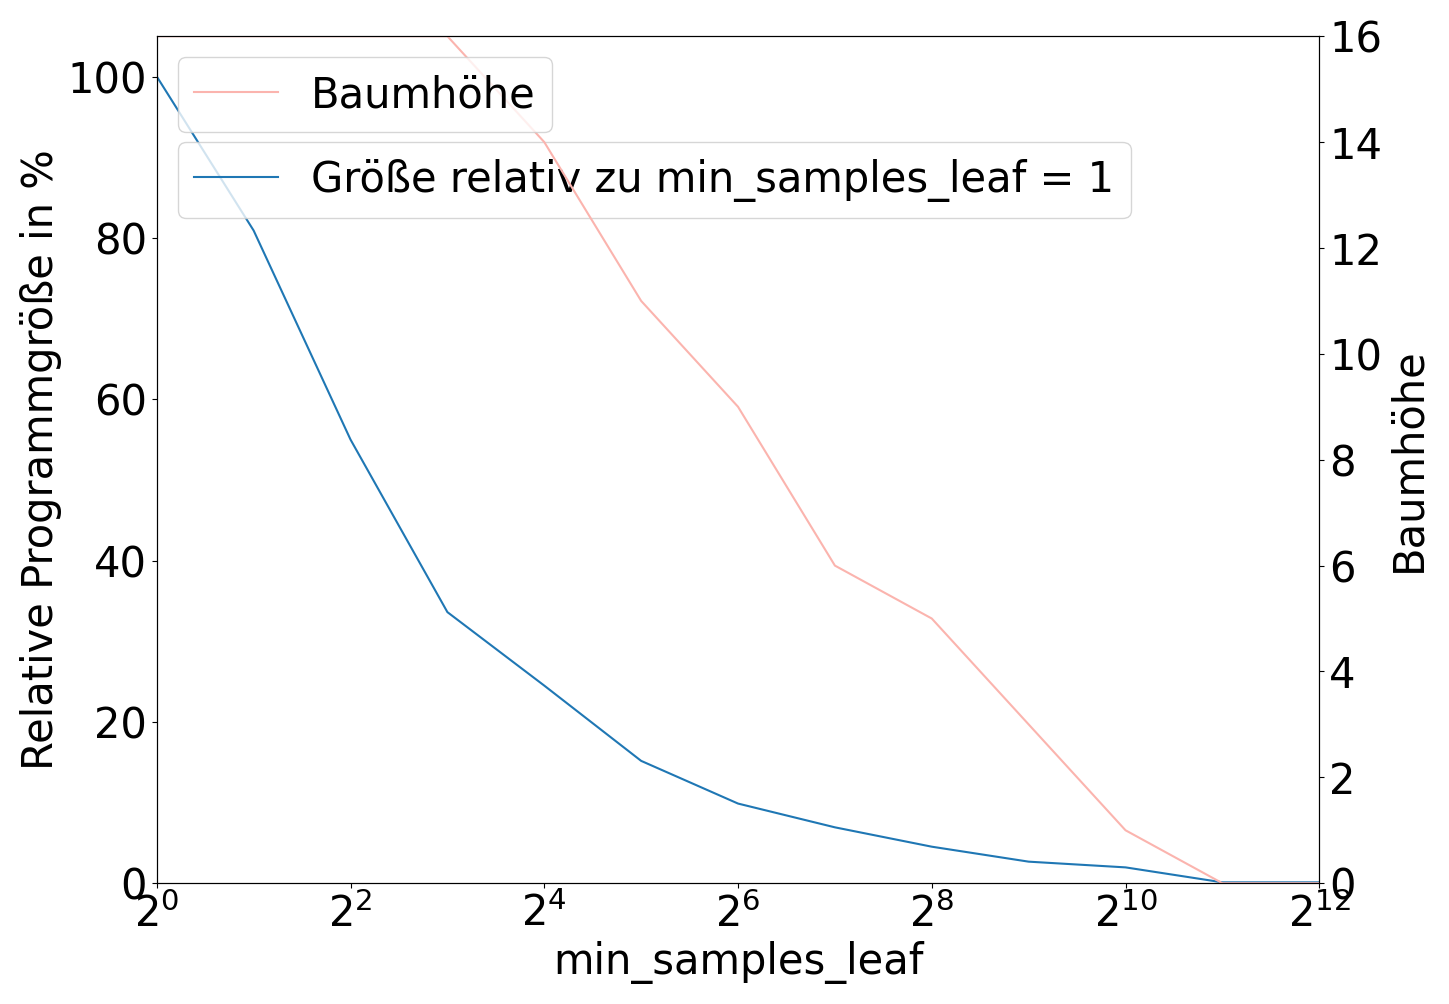
\includegraphics[width=0.48\linewidth]{images/min_samples_leaf_big.png}}%
}{Auswirkung der minimalen Blattgröße auf Programmgröße und Baumhöhe.}{fig:msl}
\newline
\newline
Es kann nicht argumentiert werden, dass ein Wert für die Blattgröße besser ist als ein Anderer, da die Klassifizierungsgenauigkeit auf der Trainingsmenge keine Aussage über die Klassifizierungsgenauigkeit auf
der Testmenge treffen kann. Eine hohe Klassifizierungsgenauigkeit auf Trainingsmenge muss nicht umbedingt eine hohe Klassifizierungsgenauigkeit auf der Testmenge implizieren. Allerdings können so vermeintlich
höhere Entscheidungsbäume ausgewählt werden, da diese weniger Programmspeicher benötigen im Vergleich zu gleich hohen Entscheidungsbäumen mit einer geringeren Blattgröße. Dieser Parameter vergrößert folglich
den Suchraum. Bei kleinen Trainingsmengen ist eine Blattgröße über 1 nur sinnvoll, wenn der größte Entscheidungsbaum, der generiert werden kann, nicht innerhalb der Restriktionen des Programmspeichers liegt.
\subsection{Minimierung der Instruktionen eines Vergleichs}
Ein Vergleich in einem Entscheidungsbaum wurde in Kapitel \ref{sec:cCodeTree} als Abzweigungsexpression mit einem Test definiert. Der Compiler erzeugt für den gleichen Programmcode verschieden viele Instruktionen
je nach Wahl des Datentyps.
\newline
\newline
Listing \ref{lst:assemblyVergleich} zeigt die Komplexität eines einzigen Vergleichs in Instruktionen eines Gleitkommazahlvergleichs. Zeile 1 bis 4 lädt die konstante Gleitkommazahl in 4 hintereinander liegende
8-Bit Register. Zeile 5 bis 7 lädt den Zeiger, der auf die Feature-Menge zeigt, und inkrementiert ihn um 36, um auf das 9. Feature zuzugreifen. In Zeile 8 bis 11 wird das Feature in die Register geladen. Zeile 12 bis 15 führen die
Vergleichsfunktion aus. Damit benötigt ein Vergleich insgesamt 15 Instruktionen.
\begin{lstlisting}[label=lst:assemblyVergleich,caption={Vergleich von Feature als Gleitkommazahl mit konstanter Gleitkommazahl.}]
01: ldi r18,lo8(33)
02: ldi r19,lo8(-92)
03: ldi r20,lo8(69)
04: ldi r21,lo8(60)
05: ldd r26,Y+5
06: ldd r27,Y+6
07: adiw r26,36
08: ld r22,X+
09: ld r23,X+
10: ld r24,X+
11: ld r25,X
12: sbiw r26,36+3
13: call __lesf2
14: cp __zero_reg__,r24
15: brge .+2
\end{lstlisting}
Zu vermeiden sind Zeile 5 bis 11, indem alle Features nur einmal in Register geladen werden. Dies ist allerdings nur möglich, wenn die Größe der Feature-Menge nicht 32~Byte übersteigt bei dem
ATmega328P. Zusätzlich müssten noch Bytes verfügbar sein, um die Konstanten zu laden. Die Feature-Menge der Schwerpunktverteilung beinhaltet 10 Einträge. Der Ansatz mit Gleitkommazahlen ist mit 40 Bytes zu groß.
Der Ansatz mit Ganzzahlen kann diese Optimierung mit 20~Byte ausnutzen. Der Compiler führt diese Optimierung bereits automatisch durch. Wenn die Feature-Menge zu groß ist, werden aus diesem Grund regelmäßig
Register verdrängt, wodurch zusätzlich Instruktionen entstehen. Die Anzahl der Instruktionen können reduziert werden, indem die Größe der Feature-Menge reduziert wird, sodass die Feature-Menge und eine
zusätzliche Konstante des gleichen Datentyps den Registerspeicher nicht übersteigen.
\newline
\newline
Der Datentyp \texttt{Float} ist sehr teuer für einen 8-Bit Prozessor, da immer 4~Register benötigt werden und gegebenenfalls zusätzliche Funktionen, die die fehlende Hardwareunterstüzung ergänzen.
Idealerweise sollte für die Feature-Menge und die Vergleiche ein 8-Bit Datentyp gewählt werden. Damit werden einerseits weniger Register benötigt, wodurch wiederrum die Feature-Menge größer sein kann,
und andererseits können hardwareunterstützte Vergleichsinstruktionen benutzt werden. Dies verringert die Anzahl der Instruktionen signifikant. Folglich vermindert ein kleinerer Datentyp die Anzahl der
Instruktionen signifikant. Listing \ref{lst:assemblyVergleich8Bit} zeigt einen Vergleich von einem 8-Bit Datentyp. Im Kontrast zum Vergleich mit Gleitkommazahlen, werden 66,6\% weniger Instruktionen
benötigt.
\begin{lstlisting}[label=lst:assemblyVergleich8Bit,caption={Vergleich von 8-Bit Feature mit konstanter 8-Bit Zahl.}]
01: adiw r26,4
02: ld r24,X
03: sbiw r26,4
04: cpi r24,lo8(124)
05: brge .L3
\end{lstlisting}
\subsection{Minimierung der Instruktionen einer Rückgabe}
Die Rückgabe der Klassifizierung in einem Entscheidungsbaum kann auf zwei Arten stattfinden. Einerseits kann lediglich die Klasse mit der höchsten Wahrscheinlichkeit zurückgegeben werden. Andererseits kann die
Wahrscheinlichkeitsverteilung zurückgegeben werden, sodass die nächste Ebene die Entscheidung trifft. In Kapitel \ref{sec:cCodeTree} wurde letzteres vorgestellt, da in der nächsten Ebene der Wahlklassifizierer
die Entscheidungsbäume im Ensemble mit Hilfe ihrer Wahrscheinlichkeitsverteilungen zusammenfasst.
\newline
\newline
Listing \ref{lst:assemblyBlattReturn} zeigt die Instruktionen die für die Zuweisung zu vier Klassen von 1.0, 0.0, 0.0 und 0.0 generiert werden. Für jede Klasse wird die Konstante Wahrscheinlichkeit in Register geladen
und anschließend in den Rückgabeparameter gespeichert. In diesem Fall muss nur für die erste Klasse eine Konstante geladen werden, da jede andere Klasse 0 ist. Das heißt, dass im schlimmsten Fall 33
Instruktionen benötigt werden, anstatt 21. Der Compiler führt hier bereits eine Optimierung aus, indem für jedes Ergebnis ein eigener \textit{Basic block} (Eine Datenstruktur die Instruktionen mit einer Annotation
zusammenfasst)erzeugt wird. Zusätzlich könnte kein C-Code generiert werden für eine Zuweisungen mit 0. Dies erfordert aber, dass der Rückgabeparameter mit 0 vorinitialisiert ist.
\newpage
\begin{lstlisting}[label=lst:assemblyBlattReturn,caption={Beispiel der Instruktionen einer Rückgabe der Wahrscheinlichkeitsverteilung eines Entscheidungsbaumes mit 4~Klassen.}]
01: ldi r24,0
02: ldi r25,0
03: ldi r26,lo8(-128)
04: ldi r27,lo8(63)
05: st Z,r24
06: std Z+1,r25
07: std Z+2,r26
08: std Z+3,r27
09: std Z+4,__zero_reg__
10: std Z+5,__zero_reg__
11: std Z+6,__zero_reg__
12: std Z+7,__zero_reg__
13: std Z+8,__zero_reg__
14: std Z+9,__zero_reg__
15: std Z+10,__zero_reg__
16: std Z+11,__zero_reg__
17: std Z+12,__zero_reg__
18: std Z+13,__zero_reg__
19: std Z+14,__zero_reg__
20: std Z+15,__zero_reg__
21: ret
\end{lstlisting}
Eine weitere Optimierung ist den Wahlklassifizierer diskret zu modellieren. Dabei wird für jede Rückgabe des Entscheidungsbaumes ein einstimmiges Ergebnis angenommen, d. h. es wird die Klasse mit der
höchsten Wahrscheinlichkeit in jedem Baum zurückgegeben und nicht mehr die Wahrscheinlichkeitsverteilung. Dadurch werden lediglich die erkannten Klassen
gezählt, anstatt die Wahrscheinlichkeitsverteilungen zu addieren. Listing \ref{lst:assemblyBlattReturnDiskret} zeigt, dass sich die Anzahl der Instruktionen für eine Rückgabe auf genau 2~Instruktionen
reduzieren. Zusätzlich kann der Compiler diese Rückgabe in Basic blocks extrahieren, wodurch lediglich eine Sprunginstruktion benötigt wird. Diese Optimierung ist bei dem diskreten Wahlklassifizierer noch
effektiver, da es genau $N$ verschiedene Rückgabewerte gibt, für $N$ mögliche Klassen. Im schlimmsten Fall reduzieren sich die Anzahl der Instruktionen pro Rückgabe um $\frac{100}{1 + 4N}$\%
und im besten Fall um $\frac{100}{1 + 8N}$\%.
\begin{lstlisting}[label=lst:assemblyBlattReturnDiskret,caption={Beispiel des Assemblycodes der Rückgabe eines diskreten Wahlklassifizierers.}]
01: ldi r24,lo8(1)
02: ret
\end{lstlisting}
Der Nachteil dieses Ansatzes ist, dass die Ergebnisse instabil werden können, wenn viele Rückgaben nur über eine knappe Mehrheit verfügen. Das ist insbesondere der Fall in Kombination mit einem hohen Wert
für die Blattgröße, da dieser die Anzahl der Blattknoten mit Einträgen aus verschiedenen Klassen potenziell erhöht. Diese Optimierung kann auf eine gefundene Lösung angewendet werden, die zu groß für den
Programmspeicher ist. Anschließend sollte die Klassifizierungsgenauigkeit revalidiert werden. Tests haben ergeben, dass die Klassifizierungsgenauigkeit geringfügig schwankt. Folglich kann sich die
Klassifizierungsgenauigkeit auf der Testmenge auch erhöhen.
\newline
\newline
Denkbar wäre ein hybrider Ansatz, der bei einem eindeutigen Ergebnis die Klasse zurück gibt und ansonsten die Wahrscheinlichkeitsverteilung. Die \glqq Eindeutigkeit\grqq\ kann über
einen Schwellenwert $\delta$ definiert sein. Ein Schwellenwert von $\delta=0$ würde an der Korrektheit nichts ändern, würde aber im schlimmsten Fall die Programmgröße nicht verringern.
Tests haben ergeben, dass es immer eindeutige Ergebnisse gibt, weswegen diese Optimierung immer angewendet werden sollte.

\chapter{Diskussion}
Der Fokus der Arbeit lag sehr früh auf der Evaluierung von verschiedenen Ensemble-Methoden und Hyperparametern. Dieser Ansatz ist aber nicht optimal, da die Ensemble-Methoden ihr potential nicht vollständig
ausnutzen konnten. Der Grund dafür ist die Wahl der Featuremengen. Im engeren Sinne sind die Featuremengen keine Featuremengen, sondern Features die aus mehreren Werten bestehen. Dementsprechend können
Ensemble-Methoden, wie Random Forests oder ExtraTrees keinen Vorteil daraus ziehen, dass sie nur Subsets der Featuremenge nutzen. Diese Ansätze funktionieren besser mit eigenständigen Feature.
\newline
\newline
Ein besserer Ansatz wäre vermutlich Stacking gewesen. Dieser Ansatz baut iterativ einen Entscheidungsbaum nach dem Anderen auf Basis der Ergebnisse der vorherigen Entscheidungsbäume und
unterschiedlichen Featuremengen. Der Vorteil ist, dass die einzelnen Featuremengen nicht so viele Anforderungen erfüllen müssen, solange alle unterschiedlichen Featuremengen zusammen alle
Anforderungen erfüllen. Dies erleichtert die Suche nach Features signifikant. Mit jedem Entscheidungsbaum können einfache Attribute inferiert werden, wie z. B. dass es eine horizontale Bewegung ist.
Im folgenden Entscheidungsbaum müsste dann lediglich die Richtung unterschieden werden. Es wird vermutet, dass der resultierende Ansatz simpler ist und kleinere Entscheidungswälder generiert.
\newline
\newline
Die momentanen Trainingsdaten wurden weitesgehend unter den gleichen Lichtverhältnissen aufgenommen. Damit sind aber nicht alle möglichen Lichtverhältnisse gut repräsentiert. Womöglich könnte ein
Teil der synthetischen Daten zur Überprüfung der Lichtverhältnisse dazu genutzt werden, um Modelle zu generieren die robuster gegenüber verschiedenen Kontrasten und Helligkeiten sind.
\chapter{Schlussfolgerungen}
Diese Arbeit hat gezeigt, dass sich Klassifizierer mit Entscheidungsbäumen sehr gut für die Handgestenerkennung eignen. Sie können, sowohl unter guten als auch
relativ schlechten Lichtverhältnissen, sehr hohe Klassifizierungsgenauigkeiten erzielen. Nullgesten können von validen Handgesten unterschieden werden. Dabei sind diese Klassifizierer signifikant
schneller als KNNs und benötigen kaum RAM zur Ausführung. Die Klassifizierungsgenauigkeit ist abhängig von dem Programmspeicher der genutzt werden darf.
\newline
\newline
Die beste Konfiguration, der Klassifizierer der kombinierten Schwerpunktverteilung, erzielte 94,8\% auf der Testmenge von Klisch, 99\% auf der Gestentestmenge und 95,8\% auf der Nullgestentestmenge. Damit
ist der Ansatz nur marginal schlechter als der beste Klassifizierer der vorherigen Arbeiten, der 98,96\% auf der Testmenge von Klisch erzielte. Die kombinierte Schwerpunktverteilung erwies sich als
äußerst robust gegenüber skalierte Helligkeiten und Helligkeiten mit einem Offset. Selbst bei geringem Kontrast erzielt der Ansatz eine hohe Klassifizierungsgenauigkeit. Die WCET beläuft
sich auf 5819 $\mu s\ \approx\ $ 5,8 ms. Der Großteil, ca. 4,5 ms, wird davon für die Berechnung der Features benötigt. Damit ist der Ansatz 9,4\% schneller, als der schnellste vorherige Ansatz.
Nach Anwendung aller Optimierungen und unter Annahme, dass Festkommazahlen keine Auswirkung auf die Klassifizierungsgenauigkeit haben, ist der Klassifizierer trotzdem zu groß für den ATmega328P.
\newline
\newline
Mit einer Beschränkung von 48 kB kann der Klassifizierer der kombinierten Schwerpunktverteilung 88,5\% auf der Testmenge von Klisch erzielen, 98,3\% auf
der Gestentestmenge und 92,5\% auf der Nullgestentestmenge bei einer Programmgröße von 35952 Byte und einer WCET von 4741,125 $\mu s\ \approx\ $ 4,7 ms. Mit der Beschränkung von 32\ kB, kann 87,5\% auf der
Testmenge von Klisch erzielt werden, 96,9\% auf der Gestentestmenge und 92,5\% auf der Nullgestentestmenge bei einer Programmgröße von 20552 Byte und einer WCET von 4680,0625 $\mu s\ \approx\ $ 4,7 ms.
\newline
\newline
Die Schwerpunktverteilung mit Ganzzahlen mit einer Programmgröße unter 28 kB hat eine WCET von 651,6875 $\mu s\ \approx\ $ 0,7 ms und ist damit 89,1\% schneller als das schnellste KNN von Giese \cite{gieseThesis}.
Dieser Ansatz erzielt bessere Ergebnisse als der kombinierte Ansatz auf den Testmengen unter gleichen Restriktionen, ist aber nicht robust gegenüber skalierten Helligkeiten.
\newline
\newline
Insgesamt benötigt die Implementierung der kombinierten Schwerpunktverteilung auf dem ATmega328P $X$(TODO) RAM. Dieser setzt sich zusammen aus $X$(TODO) zur Berechnung der Features, $X$(TODO) für den Puffer und
$X$(TODO) für die restliche Firmware. Im Puffer werden keine Bilder mehr gespeichert, sondern partiell ausgerechnete Features, d. h. im Fall der Schwerpunktverteilung, den Schwerpunkt jedes Bildes.
Dafür wird weniger Speicher pro Bild verwendet als zuvor, wodurch der Puffer größer sein kann als bei den KNNs. Die Programmgröße beträgt $X$(TODO).
\newline
\newline
Der Entscheidungsbaum bietet viel Optimierungspotenzial gegenüber der naiven Implementierung. Allein der Datentyp hat einen großen Einfluss sowohl auf die Programmgröße, als auch die Ausführungsgeschwindigkeit.
Dies ist aus der Spezifizierung des ATmega328P begründet, der nur über einen 8-Bit Prozessor ohne Module zur Verarbeitung von Gleitkommazahlen verfügt. Gleitkommazahlen sind dementsprechend sehr teuer und 8-Bit
Integer am günstigsten. Weitere Optimierungen sind Festkommazahlen und die Verwendung eines hybriden bzw. diskreten Wahlklassifizierers. Diese vergrößern jedoch den Suchraum für den besten Klassifizierer, da sie
sowohl die Programmgröße verringern als auch einen Einfluss auf die Klassifizierungsgenauigkeit haben.
\newline
\newline
Insgesamt ist es sehr aufwändig den potenziell besten Klassifizierer zu finden, da es viele Parameter gibt, die in Kombination unterschiedliche Klassifizierer produzieren. Zudem ist die
Konstruktion nicht immer deterministisch, weswegen sie als Monte Carlo Methode betrachtet werden kann. Insgesamt wurden 22528 verschiedene Konfigurationen untersucht und 28 Variationen an Features.
Darunter wurden neben der Schwerpunktverteilung, die Helligkeitsverteilung und Motion History betrachtet, die wesentlich schlechtere Klassifizierungsgenauigkeiten auf den Testmengen erzielten.
\newline
\newline
Im Laufe dieser Arbeit ist eine komplexe Infrastruktur entstanden, die die Evaluierung von Modellen zur Handgestenerkennung erleichtert. Die Infrastruktur stellt nützliche Code-Bibliotheken und verschiedene
Werkzeuge bereit. Mit einem dieser Werkzeuge wurden 14410 verschiedene Handgesten aufgenommen. Aus diesen Handgesten wurden 3 synthetische Testmengen erstellt. Die Nullgestentestmenge und die
Helligkeitstestmengen, die Kontraste und Skalierung testen. Außerdem wurde die Gestentestmenge damit erstellt.
\newline
\newline
In folgenden Arbeiten sollte untersucht werden, ob Stacking oder hierarchische Klassifizierer nicht besser geeignet sind für Klassifizierer mit Entscheidungsbäumen auf kleinen eingebetteten Systemen.
Es wird vermutet, dass dadurch simplere Klassifizierer generiert werden können, die simplere Featuremengen verwenden können. Außerdem könnte untersucht werden, ob KNNs nicht wesentlich kleiner sein
können, wenn die Features dieser Arbeit verwendet werden, anstatt die Rohdaten der Handgeste.

% Appendix
\begin{tuhhappendix}
  \chapter{Inhalt des USB-Sticks}
\begin{itemize}
    \item Latex-Quellcode und PDF dieses Dokuments
    \item Latex-Quellcode und PDF des Antrittsvortrags
    \item Latex-Quellcode und PDF des Abschlussvortrags
    \item Quellcode der gesamten Infrastruktur
    \item Dokumentation der Infrastruktur
    \item Hilfsskripte zum trainieren, validieren und generieren von Grafiken
    \item Verschiedene Versionen der Arduino-Firmware
    \item Trainingsdaten
    \item Testdaten
    \item Ergenbnisse der Modelle auf den Testdaten in Rohform
\end{itemize}
Weitere Informationen können dem README.md entnommen werden.
\end{tuhhappendix}

% Bibliography
\tuhhbibliography{thesis}

% The End
\end{document}
